\documentclass[12pt]{article}
\usepackage[utf8]{inputenc}
\usepackage{amsmath, amssymb, amsthm, bbm, mathrsfs}
\usepackage{hyperref}
\usepackage{geometry}
\usepackage{natbib}
\usepackage[linesnumbered,ruled,vlined]{algorithm2e}
\usepackage{verbatim}
\usepackage{multirow}
\usepackage{booktabs, array, threeparttable}
\usepackage{rotating}
\usepackage{graphicx}
\usepackage{subfigure}
\usepackage{float}
\usepackage{caption}
\usepackage{amsfonts}
\usepackage{xr}
\usepackage{enumitem}
\usepackage{xcolor}
\usepackage{comment}
\usepackage{bm}
\usepackage{csquotes}

% tikz setup
\usepackage{tikz}
\usetikzlibrary{shapes.geometric, arrows}
\tikzstyle{startstop} = [rectangle, rounded corners, minimum width=3cm, minimum height=2cm,text centered, text width = 3cm, draw=black, fill=red!30]
\tikzstyle{io} = [trapezium, trapezium left angle=70, trapezium right angle=110, minimum width=3cm, minimum height=1cm, text centered, draw=black, fill=blue!30]
\tikzstyle{process} = [rectangle, minimum width=3cm, minimum height=2cm, text centered, draw=black, text width=3cm, fill=orange!30]
\tikzstyle{decision} = [diamond, minimum width=3cm, minimum height=1cm, text centered, draw=black, text width = 3cm, fill=green!30]
\tikzstyle{arrow} = [thick,->,>=stealth]




\usepackage{showkeys}

\parskip 0.3cm
\parindent 0.7cm
\setlength{\parskip}{0.1cm} \linespread{1.5}
%\renewcommand\arraystretch{0.8}

\usepackage{geometry}
\geometry{left=2.5cm,right=2.5cm,top=2.5cm,bottom=3cm}

\usepackage{etoolbox}


% commands
\newcommand{\lt}{\left}
\newcommand{\rt}{\right}
\newcommand{\bd}[1]{\boldsymbol{#1}}
\newcommand{\mc}[1]{\mathcal{#1}}
\newcommand{\mf}[1]{\mathfrak{#1}}
\newcommand{\commenting}[1]{}

% renew
\renewcommand{\hat}{\widehat}
\renewcommand{\tilde}{\widetilde}
% functions
\newcommand{\Var}[1]{{\operatorname{Var}\left\{#1\right\}}}
\newcommand{\Cov}[2]{{\operatorname{Cov}\left\{#1,#2\right\}}}
\newcommand{\Corr}[2]{{\operatorname{Corr}\left\{#1,#2\right\}}}
\newcommand{\myvec}[1]{{\operatorname{vec}(#1)}}
\newcommand{\E}[1]{{\bbE\left\{#1\right\}}}
\newcommand{\Prob}[1]{{\bbP\left\{#1\right\}}}
\newcommand{\trace}[1]{{\operatorname{Tr}\left(#1\right)}}
\newcommand{\tr}[2]{\left\langle#1\, ,\, #2\right\rangle}
\newcommand{\note}[2]{{\color{#1} #2}}
\newcommand{\ind}[1]{\boldsymbol{1}\left\{#1\right\}}
\newcommand{\rank}[1]{\text{rank}{\left\{#1\right\}}}
\newcommand{\norm}[2]{\left\|#1\right\|_{#2}}
\newcommand{\normo}[1]{\left\|#1\right\|} % omitting subscript
\newcommand{\vc}[1]{\text{vec}\left\{#1\right\}}
\newcommand{\cnp}[2]{\begin{pmatrix}#1\\#2\end{pmatrix}} % choose p from n
\newcommand{\innerprod}[2]{\left\langle#1\, ,\, #2\right\rangle}
\newcommand{\indep}{\perp \!\!\! \perp}


\ifdef{\see}{\renewcommand{\see}[1]{\text{ (#1)}}}{\newcommand{\see}[1]{\text{ (#1)}}}


\newcommand{\diag}[1]{\text{\bfseries Diag}\left\{#1\right\}}

\def\boxit#1{\vbox{\hrule\hbox{\vrule\kern6pt\vbox{\kern6pt#1\kern6pt}\kern6pt\vrule}\hrule}}
\newcommand{\quickcomment}[2]{\vskip 2mm\boxit{\vskip 2mm{\color{red}\bf#1} {\color{red}\bf -- COMMENT: #2\vskip 2mm}}\vskip 2mm}
\newcommand{\modify}[2]{\vskip 2mm\boxit{\vskip 2mm{\color{blue}\bf#1} {\color{blue}\bf -- MODIFICATION: #2\vskip 2mm}}\vskip 2mm}
\newcommand{\inlinemod}[2]{{\color{#1} {(#2)}}}
%\usepackage{showkeys}

% require to load array package 
\newcolumntype{P}[1]{>{\centering\arraybackslash}p{#1}}
\newcolumntype{M}[1]{>{\centering\arraybackslash}m{#1}}




% ================ \mathcal =================
\newcommand{\cA}{{\mathcal{A}}}
\newcommand{\cB}{{\mathcal{B}}}
\newcommand{\cD}{{\mathcal{D}}}
\newcommand{\cX}{{\mathcal{X}}}
\newcommand{\cC}{{\mathcal{C}}}
\newcommand{\cG}{{\mathcal{G}}}
\newcommand{\cL}{{\mathcal{L}}}
\newcommand{\cT}{{\mathcal{T}}}
\newcommand{\cM}{{\mathcal{M}}}
\newcommand{\cN}{{\mathcal{N}}}
\newcommand{\cP}{{\mathcal{P}}}
\newcommand{\cQ}{{\mathcal{Q}}}
\newcommand{\cS}{{\mathcal{S}}}
\newcommand{\cK}{{\mathcal{K}}}
\newcommand{\cI}{{\mathcal{I}}}
\newcommand{\cF}{{\mathcal{F}}}

% ================ \mathfrak =================
\newcommand{\fX}{{\mathfrak{X}}}

% ================ \mathbb ===================
\newcommand{\bbI}{{\mathbb{I}}}
\newcommand{\bbP}{{\mathbb{P}}}
\newcommand{\bbT}{{\mathbb{T}}}
\newcommand{\bbS}{{\mathbb{S}}}
\newcommand{\bbR}{{\mathbb{R}}}
\newcommand{\bbB}{{\mathbb{B}}}
\newcommand{\bbE}{{\mathbb{E}}}
\newcommand{\bbN}{{\mathbb{N}}}
\newcommand{\bbM}{{\mathbb{M}}}
\newcommand{\bbK}{{\mathbb{K}}}
\newcommand{\bbZ}{{\mathbb{Z}}}

% ========== \boldsymbol ==========
\newcommand{\bone}{{\boldsymbol{1}}}
\newcommand{\bzero}{{\boldsymbol{0}}}

% small letter
\newcommand{\bc}{{\boldsymbol{c}}}
\newcommand{\bg}{{\boldsymbol{g}}}
\newcommand{\by}{{\boldsymbol{y}}}
\newcommand{\bsf}{{\boldsymbol{f}}}
\newcommand{\bh}{{\boldsymbol{h}}}
\newcommand{\bq}{{\boldsymbol{q}}}
\newcommand{\bw}{{\boldsymbol{w}}}
\newcommand{\bz}{{\boldsymbol{z}}}

% capital letter
\newcommand{\bA}{{\boldsymbol{A}}}
\newcommand{\bB}{{\boldsymbol{B}}}
\newcommand{\bC}{{\boldsymbol{C}}}
\newcommand{\bD}{{\boldsymbol{D}}}
\newcommand{\bE}{{\boldsymbol{E}}}
\newcommand{\bF}{{\boldsymbol{F}}}
\newcommand{\bG}{{\boldsymbol{G}}}
\newcommand{\bH}{{\boldsymbol{H}}}
\newcommand{\bI}{{\boldsymbol{I}}}
\newcommand{\bJ}{{\boldsymbol{J}}}
\newcommand{\bK}{{\boldsymbol{K}}}
\newcommand{\bL}{{\boldsymbol{L}}}
\newcommand{\bM}{{\boldsymbol{M}}}
\newcommand{\bN}{{\boldsymbol{N}}}
\newcommand{\bO}{{\boldsymbol{O}}}
\newcommand{\bP}{{\boldsymbol{P}}}
\newcommand{\bQ}{{\boldsymbol{Q}}}
\newcommand{\bR}{{\boldsymbol{R}}}
\newcommand{\bS}{{\boldsymbol{S}}}
\newcommand{\bT}{{\boldsymbol{T}}}
\newcommand{\bU}{{\boldsymbol{U}}}
\newcommand{\bV}{{\boldsymbol{V}}}
\newcommand{\bW}{{\boldsymbol{W}}}
\newcommand{\bX}{{\boldsymbol{X}}}
\newcommand{\bY}{{\boldsymbol{Y}}}
\newcommand{\bZ}{{\boldsymbol{Z}}}

% small greek
\newcommand{\bepsilon}{{\boldsymbol{\epsilon}}}
\newcommand{\btau}{{\boldsymbol{\tau}}}
\newcommand{\btheta}{{\boldsymbol{\theta}}}
\newcommand{\bgamma}{{\boldsymbol{\gamma}}}
\newcommand{\bxi}{{\boldsymbol{\xi}}}

% capital greek
\newcommand{\bTheta}{{\boldsymbol{\Theta}}}
\newcommand{\bGamma}{{\boldsymbol{\Gamma}}}
\newcommand{\bSigma}{{\boldsymbol{\Sigma}}}
\newcommand{\bDelta}{{\boldsymbol{\Delta}}}



% ============== \overline ================

% small greek
\newcommand{\oepsilon}{{\overline{\epsilon}}}
\newcommand{\otau}{{\overline{\tau}}}
\newcommand{\otheta}{{\overline{\theta}}}
\newcommand{\ogamma}{{\overline{\gamma}}}
\newcommand{\oxi}{{\overline{\xi}}}




% =============== tilde ==================

% small letter

% capital letter
\newcommand{\tA}{{\tilde{A}}}
\newcommand{\tB}{{\tilde{B}}}
\newcommand{\tC}{{\tilde{C}}}
\newcommand{\tD}{{\tilde{D}}}
\newcommand{\tE}{{\tilde{E}}}
\newcommand{\tF}{{\tilde{F}}}
\newcommand{\tG}{{\tilde{G}}}
\newcommand{\tH}{{\tilde{H}}}
\newcommand{\tI}{{\tilde{I}}}
\newcommand{\tJ}{{\tilde{J}}}
\newcommand{\tK}{{\tilde{K}}}
\newcommand{\tL}{{\tilde{L}}}
\newcommand{\tM}{{\tilde{M}}}
\newcommand{\tN}{{\tilde{N}}}
\newcommand{\tO}{{\tilde{O}}}
\newcommand{\tP}{{\tilde{P}}}
\newcommand{\tQ}{{\tilde{Q}}}
\newcommand{\tR}{{\tilde{R}}}
\newcommand{\tS}{{\tilde{S}}}
\newcommand{\tT}{{\tilde{T}}}
\newcommand{\tU}{{\tilde{U}}}
\newcommand{\tV}{{\tilde{V}}}
\newcommand{\tW}{{\tilde{W}}}
\newcommand{\tX}{{\tilde{X}}}
\newcommand{\tY}{{\tilde{Y}}}
\newcommand{\tZ}{{\tilde{Z}}}

% ================= \mathbf ====================
\newcommand{\bfD}{{\mathbf{D}}}
\newcommand{\bfP}{\mathbf{P}}


% ================== \hat ======================

\newcommand{\halpha}{{\hat{\alpha}}}
\newcommand{\hgamma}{{\hat{\gamma}}}
\newcommand{\hbeta}{{\hat{\beta}}}
\newcommand{\heta}{{\hat{\eta}}}
\newcommand{\hepsilon}{{\hat{\epsilon}}}
\newcommand{\htau}{{\hat{\tau}}}
\newcommand{\hmu}{{\hat{\mu}}}
\newcommand{\htheta}{{\hat{\theta}}}

\newcommand{\hd}{{\hat{d}}}
\newcommand{\hk}{{\hat{k}}}
\newcommand{\hs}{{\hat{s}}}
\newcommand{\hv}{{\hat{v}}}
\newcommand{\hy}{{\hat{y}}}
\newcommand{\hp}{{\hat{p}}}

\newcommand{\hD}{{\hat{D}}}
\newcommand{\hK}{{\hat{K}}}
\newcommand{\hQ}{{\hat{Q}}}
\newcommand{\hS}{{\hat{S}}}
\newcommand{\hV}{{\hat{V}}}
\newcommand{\hY}{{\hat{Y}}}


\newcommand{\hGamma}{{\hat{\Gamma}}}
\newcommand{\hTheta}{{\hat{\Theta}}}
\newcommand{\hDelta}{{\hat{\Delta}}}
\newcommand{\hSigma}{{\hat{\Sigma}}}

% ===================== \star ==================

% small greek
\newcommand{\stau}{{\tau^\star}}
\newcommand{\seta}{\eta^\star}

% capital greek
\newcommand{\sGamma}{{{\Gamma^\star}}}
\newcommand{\sTheta}{{\Theta^\star}}
\newcommand{\sDelta}{{\Delta^\star}}



% ================ \tilde ====================
\newcommand{\tgamma}{{\tilde{\gamma}}}







\newcommand\independent{\protect\mathpalette{\protect\independenT}{\perp}}
\def\independenT#1#2{\mathrel{\rlap{$#1#2$}\mkern2mu{#1#2}}}

% for flow control
\usepackage{xstring}
\newcommand{\showproof}[2]{%
    \IfEqCase{#1}{%
        {0}{}%
        {1}{#2}%
        % you can add more cases here as desired
    }[\PackageError{showproof}{Undefined option to showproof: #1}{}]%
}%
\def\showproofFlag {1}


% theorems
\newtheorem{definition}{Definition} 
\newtheorem{theorem}{Theorem} 
\newtheorem{lemma}{Lemma} 
\newtheorem{remark}{Remark} 
\newtheorem{corollary}{Corollary} 
\newtheorem{assumption}{Assumption} 
\newtheorem{example}{Example} 
\newtheorem{condition}{Condition} 
\newtheorem{proposition}{Proposition} 
\newtheorem{todo}{TODO} 
\newtheorem{strategy}{Strategy} 

\SetKwInput{KwInput}{Input}                % Set the Input
\SetKwInput{KwOutput}{Output}              % set the Output
%\@addtoreset{equation}{section}
\renewcommand{\theequation} {\arabic{section}.\arabic{equation}}

\title{Forward screening in finite population factorial experiments with many treatment levels}
\author{}
\date{}

\linespread{1.4}

\begin{document}

\maketitle

\begin{abstract}
    Factorial designs have been widely utilized and studied in many fields. Beyond the purpose of quantifying the factorial effect sizes, many factorial experiments are designed and conducted to seek the most (or the least) effective combinations of factor levels on a relevant outcome of interest subject to certain resource constraint. These demands bring new challenges to this realm, such as the well-recognized ``winner's curse" phenomenon, the overly large number of treatment groups or the methodological concerns of how to proceed under resource constraints. To handle these challenges, we propose a general workflow that incorporates several crucial components: (i) forward  screening; (ii) factor level combination selection; (iii) statistical inference over the ties. Theoretically, using a forward selection framework can achieve family-wise error rate control as well as  screening consistency in an asymptotic perspective. We prove finite sample probability bounds to justify the ability of factor level combination selection. Upon the selected results, we justify the inference procedure over the selected ties and report valid confidence intervals for estimation of the effects.  These statistical properties are further illustrated by several numerical experiments.
\end{abstract}

%\commenting{
\section{Introduction}
\subsection{Motivation and our contribution}

\inlinemod{red}{ignore the intro for now...}

Factorial designs have been widely utilized and studied in many fields, witnessing success in agricultural, industrial, and biomedical applications(\cite{wu2011experiments, zhao2021regression, egami2018causal}). The power of factorial designs lies in their ability to simultaneously accommodate multiple factors and provide informative assessments for the magnitude of main causal effects and interactions. 

In recent years, beyond the purpose of quantifying factorial effect sizes, many factorial experiments are designed and conducted to seek the most (or the least) effective combinations of factor levels on a relevant outcome of interest. For example, in cases where factors represent a set of strategies or policies, decision makers might be interested in identifying promising combinations of factor levels that can maximize the utility and produce the highest reward. As another example, when factors encode a set of characteristics or demographics (race, gender, ethnicity, etc.) for some population, researchers might have peculiar interests in determining which combination of levels is most impacted (positively or adversely) in terms of certain measurement. In general, how to accurately select these extreme groups as well as quantify the effect sizes constitutes the core of these practices. 

However, several challenges hinder the application of heuristic statistical methods. First, due to the well-recognized ``winner's curse" phenomenon, a naive peek at the combinations with the largest effect sizes might lead to overly optimistic estimates and a deficiency in the coverage rates \citep{lee2018winner, andrews2019inference}. Second, the number of treatment groups in factorial experiments are often quite large and can exponentially increase in scale as the number of factors grows, which leads to less accurate estimators or confidence intervals and prohibits the implementation of many common analytical strategies such as covariate adjustments. Moreover, beyond these methodological concerns, there are a variety of practical constraints that practitioners might wish to impose. For example, in the strategy combination example presented in the previous paragraph, it is of interest to position ourselves in a scenario where only restricted resources or budgets are available and we are confronted with a maximum limit in the total number of strategies we can apply. How to incorporate such realistic constraints in the analysis stands as another important problem. Last but not least, when entangled with a finite population discussion, the aforementioned problems are all missing pieces in the puzzle of factorial experiment theories. 

In this work, we propose a general workflow that targets the issues posited above. The procedure consists of several crucial components: (i) forward  screening; (ii) factor level combination selection; (iii) statistical inference over the ties. The  screening part plays an important role especially when the number of factors considered is large. There is a natural hierarchical structure in factorial experiments. Theoretically speaking, such structure can lend additional information gain if one exploits it cleverly. From a practical perspective, a more parsimonious model leads to more controllability in design and more interpretability in analysis. We show that using a forward selection framework can achieve family-wise error rate control as well as  screening consistency in an asymptotic perspective. The factor level combination selection is indispensable for our initial purpose of identifying most effective groups. We show that such a purpose can be achieved even if the number of factors are increasing. Lastly, we perform statistical inference over the selected ties and report valid confidence intervals for estimation of the effects. Interestingly, as demonstrated by our theoretical insights and simulation results, the forward  screening would lead to a great statistical efficiency gain on the inferential reports for the effect size of the best combinations.


\quickcomment{May 2, 2022, Lei}{
Also includes brief summary on the simulation results and case study. But haven't finished these sections.
}

\subsection{Literature review}
In the realm of factorial experiments, the factor-based regression typically serves as a dominant strategy for delivering point estimators and valid confidence regions, due to its simplicity and flexibility in real-life applications. For example, \cite{dasgupta2015causal} extended the classical notion of factorial effects to causal counterparts by introducing potential outcome framework and contrast designs.  \cite{zhao2021regression} studied the use of both saturated and unsaturated linear models for estimating the factorial causal effects. They discussed the parameter specifications of the regression models and  justified the commonly used ordinary least squares (OLS) practice from a theoretical perspective.  \cite{pashley2019causal} highlighted the desirable property of regression schemes combined with fractional factorial designs when full designs are possible due to constraints on resources such as units or cost. \cite{zhao2021covariate} explores the possibility of incorporating covariate information and applying restricted least squares (RLS) for multiple treatment experimental designs, including factorial studies as a special instance. 

A closely related thread of research in factorial designs focuses on variable screening and  screening. Powerful variable selection procedures can significantly reduce the complexity of the working model and lead to aditional benefits in statistical estimation and inference. In practice pre-screening serves as an appealing scheme for optimizing allocation and utilization of resources. To this end, \cite{wang2009forward} introduced forward regression for main effects screening and proves its screening consistency property. \cite{hao2014interaction} further included second-order interactions into the linear model and proposes a two-step procedure for ultra-high dimensional variable screening. Meanwhile, to save resources and build an interpretable model with high prediction power, variable selection or screening must be employed. \cite{haris2016convex} considered convex modelling of the factorial effects estimation and introduces strong heredity condition to achieve adaptive selection.  \cite{hao2018model} utilized a regularization scheme to tackle the curse of high dimensionality and perform valid variable screening with quadratic regression. Other works including \cite{lim2015learning, bien2013lasso}, proposed procedures for learning interactions based on $\ell_1$ regularized least squares based on a purely algorithmic perspective without statistical guarantee.

\quickcomment{May 2, 2022, Lei}{
Also include a discussion of winner's curse? How to elaborate this in factorial experiments? - Only in the ``selecting the best" section.
}

%Despite the exciting progress, various challenges still exist among the literature. Firstly, many state-of-art frameworks fail to respect the nature of factorial experiments. Factorial models are endowed with an excellent hierarchical structure. As \cite{wu2011experiments} points out, lower-order importance is typically viewed as a main principle in comparing and selecting among candidate terms. However, while many authors consider incorporating these structural information into their program by introducing heredity conditions, most are only designed for two-way interactions. Secondly, many procedures would unavoidably break down in finite population causal inference settings, where typically the data generation process deviates from the popular ``identically independent distributed(i.i.d.)" setup. Thirdly, in practice people may want to put their resources on a limited number of factor level combinations. 

%In some recent works 

%In this work we hope to ask the following question: how do we identify the best factor level combinations and quantify the effect size?  This aligns with the trend of inferential analysis on the best policies or rank statistics (like A/B testing, presidential voting, etc.). In certain experiments one might want to make further decision based on the first several largest effects. As a concrete example, a field experiment called ``Fed\_Exp" run trials to identify the employment discrimination in the US. If the government has plans to invest on eliminating discrimination induced by certain factors but it only has limited funding, one might hope to prioritize several factors that has the most significant impact on the outcome. This is related to performing inference on the order statistics, that is, testing:
%\begin{align*}
%    H_m : \gamma_{(m)} = 0.
%\end{align*}


%In this thesis we aim to propose a selection and inferential scheme on combinations of factors based on a level-wise forward regression procedure. More specifically, the scheme starts from identifying the significant main effects, then propagates to inference of interaction terms in a level-wise style that involves mainly the important factors and pre-identified significant lower-order interaction terms. This selection scheme has three main advantages: (i) it respects the hierarchical structure of the factorial effects, which prioritize main effects and lower-order interaction terms; (ii) it is compatible with the popular factor-based regression strategy for point estimators, which is the default option for many real-life applications; (iii) it achieves valid family wise error rate control and higher selection power, which benefits from the ordering-type testing procedure. We will provide rigorous theoretical justification for these three advantages as well as appropriate numerical experiments to verify the high-level implications.
%}

\subsection{Notations}  

We adopt the following notations throughout the manuscript. For asymptotic analyses, $a_N = {O}(b_N)$ denotes that there exists a positive constant $C>0$ such that $a_N \le Cb_N$. $a_N = o(b_N)$ denotes that $a_N/b_N \to 0$ as $N$ goes to infinity. $a_N =  \Theta(b_N)$ denotes that there exists positive constants $c$ and $C$ such that $cb_N\le a_N \le Cb_N$. 

For analyzing factorial effects,  we work with different level of sets. For an integer $K$, let $[K] = \{1,\cdots,K\}$. We use $\cK$ in calligraphic to denote a subset of $[K]$. For collection of such subsets or subsets of the power set of $[K]$, we use blackboard bold font for presentation,. For example, we denote $\bbM \subset \{\cK\mid \cK\subset[K]\}$ and denote the power set of $[K]$ as $\bbK$.


\section{Factorial experiment setup}
We consider a $2^K$ factorial experimental design for some $K\ge 2$, which encompasses $K$ factors with binary levels indexed by $z_k\in\{0,1\},k=1,\cdots, K$. Let $\bm{z}_{\mathcal{K}} = (z_k)_{k\in\mathcal{K}}$ index the combination of factors in $\mathcal{K}\subset[K]$, with $\bm{z}_{[K]}$ abbreviated to $\boldsymbol{z}$ specially. These factors define a collection of $Q = 2^K$ treatments, which we denote as $\mathcal{T}=\{\bm{z}=(z_1\cdots z_K)\mid z_k\in\{0,1\}, k=1,\cdots,K\}$. If for some $\bz$ we have $z_k = 1$, then we call factor $z_k$ is \textit{active}; otherwise $z_k$ is \textit{inactive}. We specially introduce the subsets $\cT_{K_0}$ of $\cT$, which contains the  combinations with at most $K_0$ factors set as active.  $N$ units are enrolled in the experiment, with $N(\bm{z})$ units in the group with the treatment $\bm{z}$. For simplicity, we can also index the treatments $\bz$ in $\cT$ using $1,\cdots,Q$ and write $\cT = [Q] $. Let $\overline{Y} = \{\overline{Y}(\bz)\}_{\bz\in\cT}$ be a vector defined as follows:
\begin{align*}
    \overline{Y}(\bz) = \frac{1}{N}\sum_{i=1}^N Y_i(\bz),\bz\in\cT.
\end{align*}
Unit $i$ has potential outcome $Y_i(\bm{z})$ if assigned to treatment $\bm{z}$. We aggregate the counterfactual outcomes into vectors $\bm{Y}_i = \{Y_i(\bz)\}_{\bz\in\cT}$ using lexicographic order. Let $Z_i$ encode the treatment that the $i$-th unit received under a random permutation. More concretely, for given $N(\bz)$, we have
\begin{align*}
    \bbP\{Z_i = \bz_j, i \in [N], j\in[Q]\} = \frac{1}{{N \choose N(\bz_1)}{N - N(\bz_1) \choose N(\bz_2)}\cdots {N - \sum_{j=1}^{Q-2}N(\bz_j) \choose N(\bz_{Q-1})} }.
\end{align*}  The observation for the $i$-th unit contains only a single realization among these potential outcomes, which we denote as $(Y_i, {Z}_{i})$. We also abbreviate $N(Z_i)$ as $N_i$ to denote the number of units for the treatment group to which the $i$-th individual is assigned.


We define factorial effects for any subset $\mathcal{K}$ of the $K$ factors following the discussion of \cite{dasgupta2015causal,zhao2021regression, wu2011experiments}.   We introduce a set of vectors $\{g_\cK\mid g_\cK\in\bbR^Q\}$ defined in the following way: for $|\cK| = |\{k\}| = 1$,
\begin{align*}
    g_\cK = \{g_\cK(\bz)\}_{\bz\in\cT}, ~ g_\cK(\bz) = \left\{
    \begin{array}{cc}
        1, & z_k = 1;  \\
        -1, & z_k = 0.
    \end{array}
    \right.
\end{align*}
For $|\cK|\ge 2$, we have
\begin{align*}
    g_\cK = (g_\cK(\bz))_{\bz\in\cT}, ~g_{\cK}(\bz) = \prod_{k\in\cK} g_{\{k\}}(\bz).
\end{align*}


It is convenient to introduce the vector of ones; in other words, we also define:
\begin{align*}
   g_\varnothing = \bone_{Q}.
\end{align*}
 $\tau_\varnothing = \frac{1}{2^K}g_\varnothing^\top \overline{Y}$ captures the total average of potential outcomes. The main effects and $k$-way interaction ($k \ge 2$) among factors in $\mathcal{K}$ are denoted by $\tau_{\mathcal{K}}$, which are defined by the inner product of $g_{\mathcal{K}}$ and $\overline{Y}$: $\tau_{\mathcal{K}} = \frac{1}{2^K} g_{\mathcal{K}}^\top \overline{Y}$. By introducing an orthonormal matrix ${G}\in\mathbb{R}^{Q\times Q}$ with columns designated to be the contrast vectors $g_\cK$'s, we can stack the corresponding effects into one vector:
 \begin{align}\label{eqn:def-factorial-effects}
     \tau = (\tau_{\mathcal{K}})_{\mathcal{K}\subset [K]} = \frac{1}{2^K}{G}^\top \overline{Y}, ~ G = (g_\cK)_{\cK\subset [K]}.
 \end{align}
See Example \ref{exp:2-3-fac-design} for an elaboration on these definitions in a $2^3$ design. For ease of presentation, we call the effect $\tau_\cK$ a \textit{parent} of $\tau_{\cK'}$ if $\cK\subset\cK'$ and $|\cK| = |\cK'| - 1$.
%\begin{remark}
%A difference in the scaling of $\tau_{\mathcal{K}}$ in \cite{dasgupta2015causal} and \cite{zhao2021regression}. The former use a uniform scaling $2^{-(K-1)}$ over all contrasts; but definition from conditional effects from \cite{zhao2021regression} have scaling $2^{-(K-k)}$ over $k$-way interactions. 
%\end{remark}


Following \cite{zhao2021regression}, we consider factor-based regression. For the saturated regression, the covariates ${X}_i$ is a vector indexed by combination of factors (equivalently, subsets of $[K]$). More precisely, ${X}_i$ is constructed from ${Z}_i = (z_{i,k})_{k=1}^K$ such that 
\begin{align*}
    {X}_{i,\mathcal{K}} = \left\{
    \begin{array}{cc}
        1, & \cK = \varnothing; \\
        \prod_{k\in\mathcal{K}}\left(2z_{i,k}-1\right), & \cK\subset [K].  
    \end{array}
    \right.
\end{align*}
Then \textit{the saturated regression} simply means regressing $Y_i$ on the full ${X}_i$. More generally, we denote a collection of combination of factors by $\bbM$, $\bbM \subset \mathbb{K} = \{\mathcal{K}\mid \mathcal{K}\subset[K]\}$. In particular, we let $\bbK_k = \{\cK\mid |\cK| = k\}$ be the collection of indices corresponding to all the $k$-way interactions. We can partition $\bbK$ as
\begin{align*}
    \bbK = \bigcup_{k=1}^K \bbK_k.
\end{align*}
 The combinations that correspond to the nonzero effects are aggregated into $\bbM^\star$, which is composed of $K$ levels of indices:
\begin{align*}
\bbM^\star = \bigcup_{k=1}^{K} \bbM_k^\star, \text{ where } \bbM_k^\star \text{ contains the nonzero effects in } \bbK_k.
\end{align*}


 \inlinemod{red}{Definition for model in factorial effects. A high level question: use the terminology ``model" or not? Keep it for now. Refine the wording when the results are ready.} For \textit{the unsaturated regression}, we only use a sub-vector of ${X}_i$ indexed by $\mathcal{K}\in\bbM$. Denote this sub-vector by ${X}_{i,\bbM}$, then the unsaturated regression over $\bbM$ translates to regressing $Y_i$ on ${X}_{i,\bbM}$. Although we do not assume the data generating process is based on linear models, to align with the terminology in linear regression, we call a collection of indices $\bbM$ a \textit{working model}.

Regarding the results, for regression over $\bbM$,  we use $\hat{\tau}(\bbM)$ denote the coefficients.   Moreover, the population version of the saturated and unsaturated regression are also of particular interest in our study. We use a non-hat counterpart ${\tau}(\bbM) $ and $\tau$ to denote the population effects over model $\bbM$. The orthogonality of $G$ implies the following fact:
\begin{lemma}
The population averages $\overline{Y}$ can be represented by the factorial effects:
\begin{align}\label{eqn:reparametrization}
    \overline{Y} = G\tau = G(\cdot, \bbM)\tau(\bbM) + G(\cdot, \bbM^c)\tau(\bbM^c).
\end{align}
\end{lemma}
Here we use $G(\cdot,\bbM)$ to denote the columns in $G$ indexed by $\bbM$. 

{
\color{red} 
\begin{remark}
(later... discussion or appendix) The above construction of covariates ${X}_i$ can be generalized by introducing a location-shift scheme as in \cite{zhao2021regression}. For a given centering vector ${\delta}=(\delta_k)_{k=1}^K$, the ${X}_i$ can be redefined as
\begin{align*}
X_{i,\mathcal{K}} = \prod_{k\in\mathcal{K}}\left(z_{i,k}-\delta_k\right),\mathcal{K}\subset [K].
\end{align*}
\end{remark}
}



\begin{example}[An explanation in the balanced $2^3$ factorial design]\label{exp:2-3-fac-design}



Suppose we have three binary factors, $z_1,z_2,z_3$, each with level $0$ and $1$. Combinations of different levels amount to $8$ treatment groups, indexed by a triple $(z_1z_2z_3)$ with $z_1,z_2,z_3\in\{0,1\}$:
\begin{align*}
\mathcal{T} = \{(000), (001), (010),(011),(100), (101), (110),(111)\}.
\end{align*}
There are $N=\sum_{z_1,z_2,z_3}N(z_1z_2z_3) = 2^3 N_0 $ units from this design, where $N(z_1z_2z_3) = N_0$ denotes the group size under treatment $(z_1z_2z_3)$. Each unit $i$ corresponds to a potential outcome vector $\bm{Y}_i = \{Y_i(z_1z_2z_3)\}_{z_1,z_2,z_3=0,1}^\top$. The  parameters of interest are the factorial effects (plus a total average for convenience) ${\tau}=\left(\tau_\varnothing, \tau_{\{1\}},\tau_{\{2\}},\tau_{\{3\}}, \tau_{\{23\}}, \tau_{\{13\}}, \tau_{\{12\}}, \tau_{\{123\}}\right)^\top$, which are defined as ${\tau} = \frac{1}{2^3} {G}^\top\overline{Y}$ through a contrast matrix ${G}$. 
\[
{G} = 
\begin{pmatrix}
1  & 1  & 1  & 1  & 1 & 1 & 1 & 1\\ 
-1 & -1 & -1 & -1 & 1 & 1 & 1 & 1\\
-1 & -1 & 1 & 1 & 1 & 1 & -1 & -1\\
-1 & 1 & -1 & 1 & -1 & 1 & -1 & 1\\
1 & 1 & -1 & -1 & 1 & 1 & -1 & -1\\
1 & -1 & 1 & -1 & -1 & 1 & -1 & 1\\
1 & -1 & -1 & 1 & -1 & 1 & 1 & -1\\
-1 & 1 & 1 & -1 & -1 & 1 & 1 & -1
\end{pmatrix}.
\]

We observe $(Y_i, {Z}_i)$ for the unit $i$, where ${Z}_i = (z_{i,1},z_{i,2},z_{i,3})$. Let $z_{i,k}' = 2z_{i,k} - 1$ be the centered version of $z_{i,k} $ .  For the purpose of regression, we construct an ${X}_i$ from ${Z}_i$:
\begin{align*}
{X}_i = \Big[&1, ~z_{i,1}', ~z_{i,2}', ~z_{i,3}',
z_{i,2}'z_{i,3}', ~z_{i,1}'z_{i,3}',  z_{i,1}'z_{i,2}', ~ z_{i,1}'z_{i,2}'z_{i,3}'\Big].
\end{align*}
Note by our general notation, we see that ${X}_i$ is defined as a vector indexed by a combination of factors or subset of $[K]$, with $K=3$ in this case. A saturated regression can then be expressed as 
\[
Y_i \sim {X}_i.
\]
Sometimes we are also interested in the unsaturated regression. For example, if we only include indices $\varnothing$ (the intercept), $\{1\},\{12\},\{13\},\{123\}$ in our regression, we can form a set of indices $\bbM=\{\varnothing, \{1\},\{12\},\{13\},\{123\}\}$ and perform
\begin{align*}
Y_i\sim {X}_{i,\bbM}, \text{ where } {X}_{i,\bbM} = &\Big[1, ~z_{i,1}', ~z_{i,1}'z_{i,2}', ~z_{i,1}'z_{i,3}', z_{i,1}'z_{i,2}'z_{i,3}'\Big].
\end{align*}
\end{example}

{\color{red} (i) Change the notation for $X$ later! Maybe to $F$. (Not $F$! Try $W$ later.) (ii) Use $X(i, \cdot)$... for unification}


\section{Motivation}

In randomized experiments, we are usually interested in estimating linear transformations of potential outcomes:
\begin{align}\label{eqn:FTY}
    \gamma = F^\top \overline{Y}
\end{align}
where $F$ is a matrix in $\in\bbR^{H\times Q}$. When the number of treatment groups are small, estimation and inference for \eqref{eqn:FTY} have been well understood \citep{li2017general, zhao2021regression, zhao2021covariate}. One important condition that is imposed across literature is:
\begin{align}\label{eqn:old-cond}
    Q \text{ is fixed}, ~ N\to\infty, ~N(\bz)/N \to e_{\bz} \in (0,1).
\end{align}

While Condition \eqref{eqn:old-cond} is able to guarantee satisfactory asymptotic results in small $Q$ regimes, it is restrictive in practice and in more complicated statistical setups. Such concern is  especially salient in factorial experiments, where the number of treatment groups is  $Q = 2^K$, which can be large in general when the number of factors is large. From a practical point of view, Condition \eqref{eqn:old-cond} requires that each arm contains a large collection of units, which might be violated in reality due to the limited resources and the difficulty of recruiting subjects. From a statistical point of view, Condition \eqref{eqn:old-cond} breaks down even if we consider a slowly growing $Q$ in asymptotic regimes.  To see this, consider a balance design where each treatment arm contains $N_0$ units ($N(\bz) = N_0$ for all $\bz\in\cT$). Then we have:
\begin{align*}
    \frac{N(\bz)}{N} = \frac{N_0}{Q * N_0} = \frac{1}{Q} \to 0, \text{ for $Q\to\infty$ with arbitrary rates}.
\end{align*}
These issues call for new ideas of analyzing factorial experiments.  


However, this does not declare the death of the story. 
One promising idea to circumvent such drawbacks is to take advantage of the special structural information in factorial experiments. As \cite{wu2011experiments} points out, there are several important principles in analyzing factorial experiments:
\begin{itemize}
    \item \textit{Effect Hierarchy Principle}.
(i) Lower-order effects are more likely to be important than higher-order effects. (ii) Effects of the same order are equally likely to be important.
    \item \textit{Effect Sparsity Principle}.
The number of relatively important effects in a factorial experiment is small.
    \item \textit{Effect Heredity Principle.}
In order for an interaction to be significant, at least one of its parent main effects
should be significant. 
\end{itemize}
These principles suggest the possibility to exploit the hierarchy and sparsity structure in the factorial effects \eqref{eqn:def-factorial-effects} to overcome the barrier of limited replications. This motivates us to perform an effect screening (or variable selection from a regression perspective) step that is tailored to the structure of factorial experiments and reduce the complexity of the model, then use the selected working model to analyze the target parameters. 

We elaborate the above ideas in several interesting examples.

\begin{example}[Inference on factorial effects with many factors]\label{exp:report-effects}
\cite{zhao2021regression} has discussed the statistical property of saturated and unsaturated linear regressions in finite population factorial experiment study:
\begin{align*}
    Y_i \sim X_{i,\bbM}, 
\end{align*}
for a pre-specified model $\bbM \subset [K]$. 

Several questions remain unclear. First, how should practioners decide $\bbM$ in real world scientific study? Second, if the number of factors $K$ is allowed to grow, how will the story change? In this case  screening is a natural requirement and directly serves for the purpose of the problem.
\end{example}


\begin{example}[Inference on general contrasts of potential outcomes]\label{exp:general-contrasts}
In many settings we are interested in testing general contrasts of average of potential outcomes:
\begin{align}
    \text{H}_0: F^\top \overline{Y} = \gamma_0. \label{eqn:H0}
\end{align}
Here $F\in\bbR^{H\times Q}$ is a general contrast matrix of interest. For example, $F$ can a vector in $\bbR^Q$ with $1$ indicating interested arms (say arms with largest average of potential outcomes or with certain factors set to particular levels like $\bz_1 = \bz_2 = 1$ which is related to conditional effects) and $0$ for the rest. Testing $\eqref{eqn:H0}$ has been well studied in classical settings.   If we are able to further screen the effects, it is possible to exploit the shared information between groups and reduce the complexity of the problem. In other words, incorporating the following information could help with the testing:
\begin{align}
 \frac{1}{2^K}G(\cdot,{\bbM^{\star c}})^\top \overline{Y} = 0. \label{eqn:constraint}
\end{align}
Again, $\bbM^\star$ is unknown to people without further exploration.  Utilizing the information $\eqref{eqn:constraint}$ is also related to the restricted least squares in a multi-arm treatment experiment \citep{zhao2021covariate}. \end{example}



\begin{example}[Select the best factor combinations]\label{exp:select-best}

In many applications, we want to identify the ''best" treatment group:
\begin{align}\label{eqn:hat-bz}
    \hat{\bz} = \underset{\bz\in\cT'\subset\cT}{\arg\max}~ \overline{Y}(z_1\cdots z_K).
\end{align}
Many traditional schemes typically are established by considering each treatment arm separately and fail to incorporate the mutual information that is shared across arms. It can be anticipated that by borrowing information from other groups, one could improve the accuracy of estimation.  screening provides one approach to achieve such a goal. To get a raw idea on this, suppose the true working model (nonzero effects) is $\bbM^\star$, we would have additional information to get $\hat{\bz}$:
\begin{align}\label{eqn:hat-bz-general}
    \hat{\bz} &= \underset{\bz\in\cT'\subset\cT}{\arg\max}~ \overline{Y}(z_1\cdots z_K), \\
    &\text{s.t. }  \frac{1}{2^K}(G_{\bbM^{\star c}})^\top \overline{Y} = 0. \notag
\end{align}
Note that here $\bbM^{\star c} $ is unknown to people.
Now the constraints reflect the between-arm information which grants the problem a lower inherent dimensionality than the original formulation. The key question is, because $\bbM^{\star c}$ is unknown to people beforehand, how should we decide the correct model to use in practice?
\end{example}



After we present the main procedure and theoretical results in Section \ref{sec:forward-framework}, we will come back and revisit these examples with more fruitful discussion.

\section{Forward screening in factorial experiments} \label{sec:forward-framework}

In this section we introduce the forward screening framework. The factorial effects have a natural hierarchical structure, which motivates a selection procedure that proceeds in a level-by-level style. Within each level, we apply some  screening methods to select nonzero effects, such as marginal t tests with Bonferroni correction, lasso, etc. Between levels, we transition from lower order effects to a pre-selected working model for higher order effects following certain logic such as heredity principles. The forward selection procedure is summarized in Algorithm \ref{alg:forward-ms}.

\begin{algorithm}[!ht]
\DontPrintSemicolon
\SetKwInput{KwInput}{Input}                % Set the Input
\SetKwInput{KwOutput}{Output}  
\SetKwFunction{MADES}{MADE-S}
\SetKwProg{Fn}{Function}{:}{\KwRet}


  \KwInput{Factorial data $(Y_i, {Z}_i)$; predetermined integer $D$; initial model for factorial effects $\hat{\bbM} = \{\varnothing\}$; significance level $\{\alpha_d\}_{d=1}^D$.}
  \KwOutput{Selected working model $\hat{\bbM}$. }
    
    Define an intermediate model $\hat{\bbM}' = \hat{\bbM}$ for convenience.
    
    \For{$d = 1,\cdots, D$}
    {
      Update intermediate model to include all the $d$-order terms: $\hat{\bbM}' = \hat{\bbM} \cup \bbK_d$.\label{alg:step-add-d-way} 
         screening
      Prune interactions according to the heredity principle \eqref{eqn:weak-heredity} or \eqref{eqn:strong-heredity} and still denote the pruned working model as $\hat{\bbM}'$.  \label{alg:step-prune}      
      
      Run weighted least squares on the model $\hat{\bbM}'$:
       \begin{align*}
          Y_i \sim X_{i, \hat{\bbM}'}, \text{ with weights } w_i = N/N_i.
       \end{align*}
    
     
      Obtain coefficients $\hat{\tau}(\hat{\bbM}')$ and robust covariance estimation $\hat{\bSigma}(\hat{\bbM}')$:
      \begin{align*}
          \hat{\bSigma}(\hat{\bbM}') = \frac{1}{Q^2}G_{\hat{\bbM}'}^\top \diag{N(\bz)^{-1}\hS(\bz,\bz)} G_{\hat{\bbM}'}.
      \end{align*} \label{alg:BC-1}
      

       Extract $\hat{\tau}_{\cK}(\hat{\bbM}')$ and $\hat{\sigma}_\cK(\hat{\bbM}')$ for all $\cK\in\hat{\bbM}'$ with $|\cK| = d$. \label{alg:BC-2}

      Run marginal t-test using the above $\hat{\tau}_{\cK}(\hat{\bbM}')$ and $\hat{\sigma}_\cK(\hat{\bbM}')$  under significance level $\min\{\alpha_d/(|\hat{\bbM}'|-|\hat{\bbM}|),1\}$ and remove the non-significant terms from $\hat{\bbM}'\backslash\hat{\bbM}$.  \label{alg:BC-3}

      Set $\hat{\bbM} = \hat{\bbM}'$.
         
    }
    
    
    \KwRet{$\hat{\bbM}$}
    
\caption{Forward  screening under heredity}
\label{alg:forward-ms}
\end{algorithm}



We briefly elaborate the high level intuition behind the forward screening procedure.  The selected $\hat{\bbM}$ can be partitioned as follows:
\begin{align*}
    \hat{\bbM} = \bigcup_{d=1}^D\hat{\bbM}_d, \text{ where } \hat{\bbM}_d = \hat{\bbM}\cap \bbK_d.
\end{align*}

One important part in understanding Algorithm \ref{alg:forward-ms} is that it introduces one operator to select models within each layer and another operator to advance the selected working model to a pre-model for the next layer. We call the within-level selection a ``S-step", which is captured by a data-dependent operator $\hat{\texttt{S}} = \hat{\texttt{S}}(\cdot;\{Y_i,Z_i\}_{i=1}^N): \{\bbM\} \to \{\bbM\}$, and the between-level proceeding a ``P-step", which is captured by a deterministic operator $\texttt{P} = \texttt{P}(\cdot): \{\bbM\} \to \{\bbM\}$.  
Concretely speaking, Step \ref{alg:step-prune} introduces a deterministic operator $\texttt{P}(\cdot)$ on a given model $\bbM$, while Step \ref{alg:BC-1} - Step \ref{alg:BC-3} introduces a stochastic (or data dependent) operator $\hat{\texttt{S}}(\cdot) = \hat{\texttt{S}}(\cdot; \{Y_i,X_i\}_{i=1}^N)$ on any given model $\bbM$. We can track the models in the following diagram:
\begin{align}\label{eqn:track-model}
    \hat{\bbM}_{1}\xrightarrow{\texttt{P}}\cdots\xrightarrow{ \hat{\texttt{S}}}\hat{\bbM}_{d-1}\xrightarrow{\texttt{P}}\hat{\bbM}_{d,+}\xrightarrow{ \hat{\texttt{S}}}\hat{\bbM}_{d}\to \cdots \xrightarrow{ \hat{\texttt{S}}} \hat{\bbM}_{D}.
\end{align}

 Note that both $\hat{\texttt{S}}(\cdot)$ and $\texttt{P}(\cdot)$ can be general. In Algorithm \ref{alg:forward-ms}, our S-step is based on marginal t tests and P-step is to proceed with one of the following heredity principles:
\begin{itemize}
\item Weak heredity: remove all the $d$-way interaction term indexed by $\cK$ from $\hat{\bbM}'$ if 
       \begin{align}
           \cK'\notin \hat{\bbM}' \text{ for all }\cK'\subset\cK,~|\cK'| = |\cK| - 1. \label{eqn:weak-heredity}
       \end{align}

\item Strong heredity: remove all the $d$-way interaction term indexed by $\cK$ from $\hat{\bbM}'$ if 
       \begin{align}
           \cK'\notin \hat{\bbM}' \text{ for some }\cK'\subset\cK,~|\cK'| = |\cK| - 1. \label{eqn:strong-heredity}
       \end{align}

\end{itemize}

In practice, one can choose $\hat{\texttt{S}}(\cdot)$ and $\texttt{P}(\cdot)$ based on the data structure as well as the background knowledge available to people. 



\section{Theoretical insights}




\subsection{General results regarding consistency of forward screening}

We are now ready to show the guarantee for our procedure. Our presentation starts from a theorem (Theorem \ref{thm:ms-consistency}) quantifying the performance of the forward procedure \eqref{eqn:track-model} under general assumptions on the S-step and P-step. Then we derive a corollary (Corollary \ref{cor:marginal-t}) by specifying the S-step as Bonferroni corrected marginal t tests and the P-step as screening based on heredity.  The high level of the proof proceeds through mathematical induction:
\begin{enumerate}
    \item (Base case) Show that forward screening selects the correct main effects with probability tending to one.
    
    \item (Induction step) Show that if we correctly screen the effects up to $k$-way interactions (main effects if $k=1$), then we are able to correctly detect the non-nulls among all $(k+1)$-way interactions. 
\end{enumerate}

\commenting{
Recall that the validity of a test requires that given the null is true, the probability of rejection should be less than the pre-specified significance level. The consistency of a test, on the other hand, requires that when the alternative is true, we have probability tending to 1 to reject the null.  Following the tradition in the realm of  screening \citep{wasserman2009high}, we introduce the following definitions:
\begin{definition}[Terminologies for  screening]
The following terminologies are wrapped up for the discussion of  screening:
\begin{itemize}
    \item Type I error:  commit a false positive. Since the selected positives are contained in $\hat{\bbM}$, this translates into $\hat{\bbM}\cap\bbM^{\star c}\neq \varnothing$. 
    \item Type II error:  commit a false negative. Since the selected negatives are contained in $\hat{\bbM}$, this translates into $\hat{\bbM}^c\cap\bbM^{\star}\neq \varnothing$. 
\end{itemize}
\end{definition}

Clearly size measures the ability of under-selection; since zero $q(\hat{\bbM})$ means $\hat{\bbM}\subset \bbM^\star$. Power measures the ability of over-selection, since a power of 1 means $\bbM^\star\subset\hat{\bbM}$. We have the following graph to visualize the idea:



%\tikzset{every picture/.style={line width=0.75pt}} %set default line width to 0.75pt        
\begin{figure}[th]
\centering


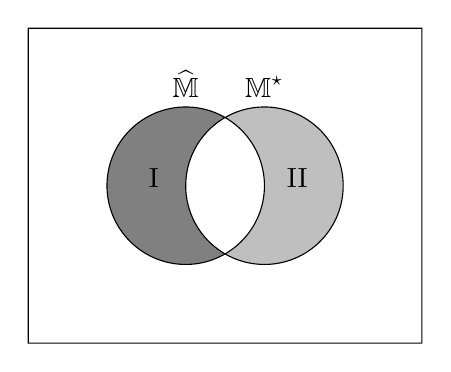
\begin{tikzpicture}[fill]
% left hand
\scope
\clip (-2,-2) rectangle (2,2)
      (1,0) circle (1);
\fill[gray] (0,0) circle (1);
\endscope
% right hand
\scope
\clip (-2,-2) rectangle (2,2)
      (0,0) circle (1);
\fill[lightgray] (1,0) circle (1);
\endscope
% outline
\draw (0,0) circle (1) (0,1)  node [text=black,above] {$\displaystyle \hat{{\bbM}}$}
      (1,0) circle (1) (1,1)  node [text=black,above] {$\displaystyle {\bbM}^{\star}$}
      (-2,-2) rectangle (3,2);
      
% Text Node
\draw (1.25,0.25) node [anchor=north west][inner sep=0.75pt]   [align=left] {II};
% Text Node
\draw (-0.5,0.25) node [anchor=north west][inner sep=0.75pt]   [align=left] {I};
      
      
      
\end{tikzpicture}
\label{fig:error-visual}
\caption{Visualization of the two types of errors} screening

\end{figure}
}


In order to achieve satisfactory screening results, some regularization conditions need to be imposed to characterize a ``good" layer-wise S-step, and the P-step should ensure that the procedure progress in a way that is compatible with the structure of the true factorial effects.  In light of this, we use ${\bbM}^\star_{d,+}$ to denote the pruned set of effects on the $d$-th layer based on the true model $\bbM_{d-1}^\star$ on the previous layer; that is,
\begin{align*}
    {\bbM}^\star_{d,+} = \texttt{P}({\bbM}^\star_{d-1}).
\end{align*}
These discussions motivate the following assumption on the layer-wise selection procedure $\hat{\texttt{S}}(\cdot)$:
\begin{assumption}[Validity and consistency of the selection operator]\label{asp:valid-consistent}
We denote 
\begin{align*}
    \tilde{\bbM}_{d} = \hat{\text{\em \texttt{S}}}(\bbM^{\star}_{d,+};\{Y_i,Z_i\}^N_{i=1}),
\end{align*}
where $\bbM^{\star}_{d,+} = \text{\em \texttt{P}}(\bbM^{\star}_{d-1})$ is defined as above. Let $\{\alpha_d\}_{d=1}^D$ be a sequence of significance levels in $(0,1)$. We assume that the following \emph{validity} and \emph{consistency} property hold for $\text{\em \texttt{S}}_N(\cdot)$: for $d = 1,\cdots, D$, we have
\begin{align}
    \text{Validity:}&~\lim\sup_{N\to\infty}\bbP\lt\{\tilde{\bbM}_{d}\cap\bbM^{\star c}_d\neq \varnothing\rt\}\le \alpha_d,  \label{eqn:validity}\\
    \text{Consistency:}&~\lim\sup_{N\to\infty}\bbP\lt\{\tilde{\bbM}_{d}^c\cap\bbM^{\star}_d\neq \varnothing\rt\} = 0.  \label{eqn:consistency}
\end{align}
\end{assumption}
\inlinemod{red}{Just out of curiosity: what is the difference between an assumption and a condition?}


This assumption can be verified for many  screening procedures. In Corollary \ref{cor:marginal-t} we will show it holds for the layer-wise Bonferroni corrected marginal testing procedure in Algorithm \ref{alg:forward-ms}. Moreover, in the high dimensional super population study, a combination of data splitting, adaptation of $\ell_1$ regularization and marginal t tests can also fulfill such a requirement \citep{wasserman2009high}.




Besides, we assume the $\texttt{P}(\cdot)$ operator respects the structure of the nonzero factorial effects:
\begin{assumption}[P-heredity]\label{asp:P-heredity}
For $d=1,\cdots,D-1$, it holds
\begin{align*}
\bbM^\star_{d+1}\subset\texttt{\em P}(\bbM^\star_{d}).
\end{align*}
\end{assumption}

One special case of $\texttt{P}(\cdot)$ operator satisfying Assumption \ref{cond:P-heredity} is naively adding all the the higher order interactions regardless of the lower-order screening results. Besides, if we have evidence that the effects have particular hierarchical structure, applying the corresponding heredity principle such as \eqref{eqn:weak-heredity} or \eqref{eqn:strong-heredity} can improve screening accuracy as well as interpretability of the screening results.
\begin{theorem}[Screening consistency]\label{thm:ms-consistency}
\inlinemod{blue}{will go to the Appendix... or not?}
Assume $\bbM^\star\neq\varnothing$. Assume Assumption \ref{asp:valid-consistent} and \ref{asp:P-heredity}.  Then the forward screening procedure \eqref{eqn:track-model} has the following properties:

\begin{enumerate}
    \item {\em Type I error control.} Forward screening controls the Type I error rate, in the sense that 
    \begin{align}
        \underset{N\to\infty}{\lim\sup}~\bbP\left(\hat{\bbM}_d\cap{\bbM_d^\star}^c\neq\varnothing \text{ for some } d\in [D]\right)\le \alpha = \sum_{d=1}^D \alpha_d.
    \end{align}
    \item {\em  Screening consistency.} Further assume $\alpha=\alpha_N\to0$. The forward procedure consistently selects all the nonzero effects up to $D$ levels with probability tending to 1: 
    \begin{align}
        \underset{N \to \infty}{\lim\sup}~\bbP\left(\hat{\bbM}_d = \bbM_d^\star \text{ for all }d\in[D]\right)=1.
    \end{align}
\end{enumerate}
\end{theorem}

{
\color{blue}
Theorem \ref{thm:ms-consistency} consists of two parts. First, one can control the type I error rate, which is defined as the probability of over-selects at least one zero effect. The definition is introduced and elaborated detailedly in \cite{wasserman2009high} for model selection. Second, if the tuning parameter $\alpha = \sum_{d=1}^D\alpha_d$ vanish asymptotically, one can actually achieve perfect screening up to $D$ levels of effects.  To apply Theorem \ref{thm:ms-consistency} to specific procedures, the key step is to verify Assumption \ref{asp:valid-consistent} and justify Assumption \ref{asp:P-heredity}, which we will do for Bonferroni corrected marginal t tests as an example in the next section.

Moreover, the scaling of $\alpha_N$ plays an important role in theoretical discussion. To achieve perfect selection, we hope $\alpha_N$ decays as fast as possible; ideally if $\alpha_N$ equals zero then we do not commit any type I error (or equivalently, we will never select redundant effects). However, for many data-dependent selection procedure $\alpha$ can only decay at certain rates, because a fast decaying $\alpha$ means higher possibility of rejection, thus can lead to strict under-selection. Therefore, in the tuning process, $\alpha_d$ should be scaled properly if one wants to pursue perfect selection. Nevertheless, even if the tuning is hard and perfect model selection can not be achieved, we still have many strategies to exploit the advantage of the forward screening procedure. We will have more discussions in later sections.
}



\subsection{Consistency of forward screening based on marginal t tests}

In this paper we consider the following \textit{nearly uniform design}:
\begin{condition}[Nearly uniform design]\label{cond:uniform-design} There exists an positive integer $N_0 > 0$ and absolute constants $\underline{c} \le \overline{c}$, such that 
\begin{align*}
    N_\bz = c_\bz  {N}_0 \ge 2,  \text{ where } \underline{c}\le c_\bz\le \overline{c}.
\end{align*}
\end{condition}

\begin{condition}[Hierarchical structure in factorial effects]\label{cond:heredity} The nonzero factorial effects have one of the following hierarchical structure:
\begin{itemize}
\item Weak heredity: $\tau_\cK\neq 0$ only if there exists $\cK'\subset\cK,~|\cK'| = |\cK| - 1$ such that $\tau_{\cK'}\neq 0$.

\item Strong heredity: $\tau_\cK\neq 0$ only if for all $\cK'\subset\cK,~|\cK'| = |\cK| - 1$, $\tau_{\cK'}\neq 0$.

\end{itemize}

\end{condition}

\begin{condition}[Order of parameters]\label{cond:order}
The true parameters and tuning parameter has the following order:
\begin{itemize}
    \item True parameter: $|\tau_\cK| =  \Theta(N^\delta)$ for some $\delta > -1/2$ and all $\cK\in\bbM_d^\star$.
    \item Tuning parameter: ${\alpha_d} =  \Theta(N^{-\delta'})$ for some $\delta'\ge 0$.
\end{itemize} 
\end{condition}

\begin{condition}[Nondegenerate correlation matrix]\label{cond:nondegenerate-corr}
Let $V^\star$ be the correlation matrix of $\hat{Y}$. There exists a $\sigma > 0$, such that \inlinemod{red}{i) a definition of $V^\star$ earlier; (ii) introduce condition number...}
    \begin{align}\label{eqn:nondegenerate-var}
        \varrho_{\min}(V^\star)/\varrho_{\max}(V^\star) \ge \sigma^2.
    \end{align}
\end{condition}

\begin{condition}[Bounded fourth moments]\label{cond:bounded-moments}
There exists a $ \Delta > 0$ such that
\begin{align}\label{eqn:bounded-moments}
   \max_{\bz\in[Q]}\frac{1}{N}\sum_{i=1}^N \{Y_i(\bz) - \overline{Y}(\bz)\}^4 \le \Delta^4.
\end{align}


\end{condition}


\begin{corollary}[Bonferroni corrected marginal test]\label{cor:marginal-t}
Let $\tilde{\bbM}_{d} = \hat{\texttt{\em S}}(\bbM^{\star}_{d,+})$ where $\bbM^{\star}_{d,+} = \texttt{\em P}(\bbM^{\star}_{d-1})$. Assume Conditions \ref{cond:uniform-design}, \ref{cond:heredity}, \ref{cond:order}, \ref{cond:nondegenerate-corr} and \ref{cond:bounded-moments}. Then we have
the following results for the  screening procedure based on Bonferroni corrected marginal t-test:
\begin{enumerate}
    \item (Validity) $\lim\sup_{N\to\infty}\bbP\lt\{\tilde{\bbM}_{d}\cap\bbM^{\star c}_d\neq \varnothing\rt\}\le \alpha_d$ for all $d=1,\cdots,D$.
    \item (Consistency) $\lim\sup_{N\to\infty}\bbP\lt\{\tilde{\bbM}_{d}^c\cap\bbM^{\star}_d\neq \varnothing\rt\} = 0$ for all $d=1,\cdots,D$.
    \item (Type I error control) Overall the procedure achieves type I error rate control:
    \begin{align*}
    \underset{N\to\infty}{\lim\sup}~\bbP\left(\hat{\bbM}\cap{\bbM^\star}^c\neq \varnothing\right)
    %\le 
    %\frac{\alpha_1}{K}\cdot|\bbM_1^\star| + \sum_{d=2}^D \frac{\alpha_d}{|\bbM^\star_{d,+}|}\cdot|\bbM^\star_d| 
    \le \alpha.
    \end{align*}
    \item (Perfect selection) When $\delta' $ is strictly positive \inlinemod{red}{not exactly Condition \ref{cond:order}! $\delta'=0$ is excluded here}, we have $\alpha_d\to0$ and
    \begin{align*}
    \underset{N\to\infty}{\lim}~\bbP\left(\hat{\bbM} = {\bbM^\star}  \right)
     = 1.
    \end{align*}
\end{enumerate}

\end{corollary}

\inlinemod{red}{Some explanation on this...}


\section{Benefits of perfect screening}
\subsection{General implications of perfect screening}
\inlinemod{red}{Why change notation to $\bw$? Explain or change...}
In the motivation section, we discussed the possible benefits that effects screening can bring to estimation and inference in factorial experiments. In this section we formalizing the ideas into theoretical results. The general target is to analyze a type of parameter that can be expressed as the linear combination of all the average potential outcomes:
\begin{align}
\gamma = \sum_{\bz\in\cT} \bw(\bz)\overline{Y}(\bz). \label{eqn:target-gamma}
\end{align}
 Consider an estimator of the form
\begin{align}\label{eqn:hgamma}
    \hgamma = \sum_{\bz\in\cT} \bw(\bz)\hat{Y}(\bz),
\end{align}
with variance estimation
\begin{align}\label{eqn:hv2R}
    \hat{v}^2_R = \sum_{\bz\in\cT} \bw(\bz)^2 \hat{S}(\bz,\bz).
\end{align}
One can verify that 
\begin{align}
    \bbE\{\hgamma\} &= \sum_{\bz\in\cT} \bw(\bz)\overline{Y}(\bz) = \gamma, \label{eqn:mean-hgamma}\\
    \Var{\hgamma} &= \sum_{\bz\in\cT}\bw(\bz)N_{\bz}^{-1}S(\bz,\bz) - N^{-1}S_\bw, \label{eqn:var-hgamma}\\
    \bbE\{\hat{v}_R^2\} & =  \sum_{\bz\in\cT} \bw(\bz)N_{\bz}^{-1}S(\bz,\bz). \label{eqn:mean-varR}
\end{align}

What is the benefits of  screening? Intuitively speaking, if we want to do inference on $\gamma = \E{\hgamma}$ given by \eqref{eqn:mean-hgamma}, one can reparameterize the parameter using  decomposition \eqref{eqn:reparametrization}. If for some $\bbM$, $\tau(\bbM^c)$ is negligible, then we could reduce the dimension of the parameter space. 

Let $\bw = (\bw(\bz))_{\bz\in[Q]} $. Define 
\begin{gather*}
    \hgamma({\bbM}) = \bw^\top G(\cdot, {\bbM}) \htau({\bbM}), ~\gamma(\bbM) = \bw^\top G(\cdot,\bbM)\tau(\bbM), \\
    v^2(\bbM) =  \bw^\top G(\cdot,\bbM)\Var{\htau(\bbM)} G(\cdot,\bbM)^\top\bw.
\end{gather*}


With perfect  screening, we have the following result:
\begin{theorem}[Berry-Esseen bound under perfect  screening]\label{thm:be-perfect-ms}
Let $ \tilde{\bw}$ be given by \eqref{eqn:tw}. Assume \eqref{eqn:nondegenerate-var-tw}. 
Then it holds
\begin{align}\label{eqn:be-perfect-ms}
    &\sup_{t\in\bbR}\lt|\Prob{\frac{\hgamma(\hat{\bbM})-\gamma}{v(\bbM^\star)} \le t} - \Phi(t)\rt| \notag\\
    &\le 2\Prob{\hat{\bbM}\neq \bbM^\star} +  2C\sigma_w   \frac{\underline{c}^{-1} \max_{i\in[N],\bz\in[Q]}|Y_i(\bz)-\overline{Y}(\bz)|}{\sqrt{\overline{c}^{-1} \min_{\bz\in[Q]} S(\bz,\bz)}\cdot \sqrt{N_0}}\cdot  \frac{\|\tilde{\bw}_{\bbM^\star}\|_\infty}{\|\tilde{\bw}_{\bbM^\star}\|_2} .
\end{align}
\end{theorem}


To further understand what benefits  screening can bring us, we make some simple comparison based on  concrete choices of $\bw$. We focus on comparing the asymptotic results: (i) under what conditions will we have CLT? (ii) how large is the limit of the robust variance (which determines the length of the confidence interval)? For simplicity we assume the potential outcomes are upper bounded and $\min_{\bz\in[Q]} S(\bz,\bz)$ is lower bounded by some universal constants. 


\begin{example}[Sparse $\bw$]
Let $\bw = (1,0,\dots,0)^\top$. Then we can compute
\begin{align*}
    \|\tilde{\bw}_{\bbM^\star}\|_\infty = Q^{-1}|\bbM^\star|, \|\tilde{\bw}_{\bbM^\star}\|_2 = \sqrt{|\bbM^\star|/Q}.
\end{align*}
Apply Theorem \ref{thm:be-perfect-ms}, we can formulate the conditions for CLT in Table \ref{tab:sparse-bw}. We can see that when $Q$ is large and $\bbM^\star$ is sparse, CLT with  screening holds under weaker conditions and the robust variance is smaller in expectation. Concretely speaking, although the coefficient $\bw$ is only associated with treatment arm $\bz=1$, by  screening we can actually incorporate information from other arms to establish CLT and variance estimator under weaker conditions. This sparse $\bw$ example plays an important role in analyzing Example \ref{exp:select-best}.
\begin{table}[!ht]
    \centering
    \caption{Comparison of conditions for CLT and limit of variance estimate for sparse $\bw$}
    \label{tab:sparse-bw}
    \begin{tabular}{cP{5cm}P{7cm}}
    \toprule
       Perfect selection  &  CLT & $\E{\hv_R^2}$ \\\midrule
        Yes &   $\Prob{\hat{\bbM} = \bbM^\star} \to 1$ and $\frac{|\bbM^\star|}{QN_0}\to 0$   & $\sum_{\bz=1}^{Q}\frac{\tilde{\bw}^2(\bz)S(\bz,\bz)}{N(\bz)}$, upper bounded by $ \frac{|\bbM^\star|}{Q}\max_{\bz\in[Q]}\{\frac{S(\bz,\bz)}{N(\bz)}\} $ \\\midrule
        No  &   $\frac{1}{N(1)}\to 0$   & $\frac{S(1,1)}{N(1)}$\\
    \bottomrule
    \end{tabular}
\end{table}
\end{example}

\begin{example}[Dense $\bw$] \inlinemod{red}{less interesting... should we still keep this? - Simulation!}
Let $\bw = Q^{-1}G(\cdot,\bbM_1\cup\bbM_2) b$ where $b\in\bbR^{K(K+1)/2}, \|b\|_2=1$ be a linear combination of the contrast vectors of the  main effects and two-way interactions. With  screening, we can compute
\begin{align*}
\tilde{\bw}_1 = Q^{-1}G(\cdot, \bbM_1^\star\cup\bbM_2^\star)\boldsymbol{b}, ~\|\tilde{\bw}_1 \|_\infty\le Q^{-1}\sqrt{|\bbM_1^\star|+|\bbM_2^\star|},~\|\tilde{\bw}_1 \|_2 = \sqrt{Q^{-1}}.
\end{align*}
Without  screening, we have
\begin{align*}
\tilde{\bw}_2 = Q^{-1}G(\cdot, \bbM_1 \cup\bbM_2 )\boldsymbol{b}, ~\|\tilde{\bw}_2 \|_\infty\le Q^{-1}\sqrt{|\bbM_1 |+|\bbM_2 |},~\|\tilde{\bw}_2 \|_2 = \sqrt{Q^{-1}}.
\end{align*}
The results are concluded in Table \ref{tab:dense-bw}. 
\begin{table}[!htbp]
    \centering
    \caption{Comparison of conditions for CLT and limit of variance estimate for dense $\bw$}
    \label{tab:dense-bw}
    \begin{tabular}{cP{5cm}P{7cm}}
    \toprule
        screening  &  CLT & $\E{\hv_R^2}$ \\\midrule
        Yes &   $\Prob{\hat{\bbM} = \bbM^\star} \to 1$ and $\frac{|\bbM^\star_1| + |\bbM^\star_2| }{QN_0}\to 0$   & $\sum_{\bz=1}^{Q}\frac{\tilde{\bw}_1^2(\bz)S(\bz,\bz)}{N(\bz)}$, upper bounded by $ \frac{1}{Q}\max_{\bz\in[Q]}\{\frac{S(\bz,\bz)}{N(\bz)}\} $ \\\midrule
        No  &   $\frac{K(K+1)}{2QN_0}\to 0$   & $\sum_{\bz=1}^{Q}\frac{\tilde{\bw}_2^2(\bz)S(\bz,\bz)}{N(\bz)}$, upper bounded by $ \frac{1}{Q}\max_{\bz\in[Q]}\{\frac{S(\bz,\bz)}{N(\bz)}\} $ \\
    \bottomrule
    \end{tabular}
\end{table}
We can see in the dense $\bw$ case, the CLT holds under slightly weaker conditions if the number of nonzero effects is small.  The variance estimation results are hard to compare directly; but the worst case upper bound does not suggest a large difference. Nevertheless,  screening can introduce heredity structure into the selected working model and add more interpretability to the results.

\end{example}

More generally one can show that
\begin{align*}
    \frac{\|\tilde{\bw}(\bbM^\star)\|_\infty}{\|\tilde{\bw}(\bbM^\star)\|_2} \le \min\lt\{\frac{|\bbM^\star|\|\bw^\top G(\cdot,\bbM^\star)\|_\infty}{\sqrt{Q}\|\bw^\top G(\cdot,\bbM^\star)\|_2},1\rt\}.
\end{align*}
Therefore, when $Q$ is large and $\bbM^\star$ is sparse, one can often expect an improvement in the Berry Esseen bound with a step of  screening. 



\quickcomment{Lei}{With Theorem \ref{thm:be-perfect-ms}, Example \ref{exp:report-effects} and \ref{exp:general-contrasts} seem trivial? Do we need to add more discussion on these two examples here? - Say why they are intuitive and what people should do.}

\subsection{Application: select the best factor combinations} 

\inlinemod{red}{needs better motivation and explanation... maybe use the charity donation example? maybe talk about winner's curse?}

We study Example \ref{exp:select-best} in this section. Concretely speaking, our goal is: (i) identify the treatment arms that demonstrates the ``best" performance measured by level of average potential outcome; (ii) do inference on the average potential outcome for the selected arms. For ease of presentation, we focus on selecting the maximal potential outcome in this section and defer discussions on general ordered average potential outcomes to the appendix. 

Denote the maximal average of potential outcome as $\overline{Y}_{(1)}$, which is achieved by a set of treatment arms $\cT_{1}$:
\begin{align}\label{eqn:near-tie}
    \cT_{1} = \lt\{\bz\in\cT'\subset \cT\mid|\overline{Y}(\bz) - \overline{Y}_{(1)}| =  \Theta(N^{-\delta_3})\rt\},  \text{ for some } \delta_3 > 0.
\end{align}
Here $\cT'$ is a subset of $\cT$. In practice $\cT'$ incorporate people's decision on which arms are interesting for comparison. As a naive example, when the number of arms is not very large, one can simply take $ \cT' = \cT$. As a less trivial example, if the $K$ different factors represent strategies that one can take, and due to resource constraint at most $K_0$ factors can be set as ``active" (meaning $z_k = 1$), then 
\begin{align*}
\cT' = \lt\{\bz\in[Q]\mid \sum_{k=1}^{K_0}z_k \le K_0\rt\}.
\end{align*}


With the above basic setup, the procedure \inlinemod{red}{turn this into an algorithm?} is formulated as follows:
\begin{enumerate}
    \item Perform effects selection with Algorithm \ref{alg:forward-ms} and obtain working model $\hat{\bbM}$.
    \item  Obtain reparametrization-based estimates:
      \begin{align*}
           \hat{Y}_{\operatorname{RP}}(\cdot) = G(\cdot,{\hat{\bbM}}) \htau(\hat{\bbM}).
      \end{align*}
    \item  Select the best factor level combinations. 
    \begin{align*}
          \hat{\cT}_{1} = \lt\{\bz\in\cT'\mid -\eta_{L,N}\le \hY_{\operatorname{RP}}(\bz)-\max_{\bz'\in\cT' }\hY_{\operatorname{RP}}(\bz') \le \eta_{R,N}\rt\}.
      \end{align*}
      Here $\eta_{L,N},\eta_{R,N}>0$ are some tuning parameters.
    \item Generate point estimates for the effect size over the $h$-th tier by taking average:
      \begin{align*}
         \hY_{(1)} = \frac{1}{|\hat{\cT}_{1}|} \sum_{\bz\in \hat{\cT}_{1}} \hY_{\operatorname{RP}}(\bz). 
      \end{align*}

\end{enumerate}










Now we define
\begin{align*}
    d_h = \max_{\bz\in\cT_{1} } |\overline{Y}(\bz) - \overline{Y}_{(1)}|, ~d^\star_h = \min_{\bz\notin\cT_{1}} |\overline{Y}(\bz) - \overline{Y}_{(1)}|.
\end{align*}
which we refer to as within-group distance and between-group distance respectively. 

For theoretical interests, we quantify the order of the involved quantities:
\begin{condition}[Order of distance]\label{cond:distance}
Assume the following scaling of parameters: $d_h^\star= \Theta(N^{\delta_1}),  \eta_{L,N} = \Theta(\eta_N),  \eta_{R,N} = \Theta(\eta_N)$ with $\eta_N = \Theta(N^{\delta_2}), d_h = \Theta(N^{\delta_3})$ with $-1/2 < \delta_3 < \delta_2 < \delta_1 \le 0$.

\end{condition}





\begin{theorem}[Consistency of the selected tie sets]\label{thm:wt-converge}
Assume Conditions \ref{cond:nondegenerate-corr} and \ref{cond:distance}.  When $N>n(\delta_1,\delta_2,\delta_3)$, it holds that
\begin{align*}
   \bbP\lt\{\hat{\cT}_{1} = {\cT}_{1} \rt\} 
   \ge&  1 - \bbP\{\hat{\bbM}\neq \bbM^\star\}\\
    -& C|\cT'||\cT_{1}|\lt\{\sqrt{\frac{\bar{c}\bar{s}|\bbM^\star|}{N^{1+2\delta_2}}}\exp\lt(-\frac{C'N^{1+2\delta_2}}{\bar{c}\bar{s}|\bbM^\star|}\rt)+\sigma   \frac{ \underline{c}^{-1} \max_{i\in[N],\bz\in[Q]}|Y_i(\bz)-\overline{Y}(\bz)|}{ {\overline{c}^{-1/2} \{\min_{\bz\in[Q]} S(\bz,\bz)}\}^{1/2}}\cdot \sqrt{\frac{|\bbM^\star|}{N_0Q}}\rt\}.
\end{align*}


\end{theorem}

\commenting{
\begin{remark}
To show the results, we assumed a delicate characterization of the distributional convergence rates in \eqref{eqn:berry-esseen}. In many cases, this corresponds to a Berry-Esseen type inequality; for example, \cite{shao2012jackknife, bentkus1996bberry, jing2000berry} proves bounds for i.i.d. data, and \cite{bolthausen1984estimate} for bounds of combinatorial type.
\end{remark}
}

\inlinemod{red}{Some words explanation?}




\begin{corollary}[Asymptotic results on the estimated effects]\label{cor:infer-order}
Assume Condition \ref{cond:nondegenerate-corr} and \ref{cond:distance}. Assume
\begin{align*}
  \Prob{\hat{\bbM} = \bbM^\star} \to 1, ~ \frac{|\bbM^\star|}{N^{1+2\delta_2}}\to 0, ~|\cT'||\cT_1|\lt(\frac{\bbM^\star}{N}\rt)^{1/2} \to 0.
\end{align*}
Then the point estimates are asymptotically jointly normal:
\begin{align*}
      \frac{ \hY_{(1)}  -   \overline{Y}_{(1)}}{(\bw^\top S \bw)^{1/2}} \to N(0, 1), 
\end{align*}
where $\bw\in\bbR^{Q}$ has columns
\begin{align*}
    \bw = \sum_{\bz\in {\cT}_{1}}\frac{{\bw}_{\bz}}{|{\cT}_{1}|} = (Q|{\cT}_{1}|)^{-1}\sum_{\bz\in {\cT}_{1}}G(\cdot,{\bbM^\star}) G({\bz, \bbM^\star})^\top .
\end{align*}
Moreover, under Condition \ref{cond:bounded-moments}, $\bw^\top \hat{S} \bw$ is a robust variance estimator for $\bw^\top S \bw $ which satisfies
\begin{align*}
    {N} (\bw^\top \hat{V}_Y \bw - \bw^\top \bbE\{\hV_Y\}\bw)\xrightarrow{\bbP} 0,  ~ \bw^\top \bbE\{\hV_Y\} \bw \succeq \bw^\top V_Y \bw.
\end{align*}

\end{corollary}
\inlinemod{red}{Need to polish the proof.}

\textbf{Benefits of reparametrization under sparsity.}  Note that Theorem \ref{thm:wt-converge} and Corollary \ref{cor:infer-order} can actually incorporate both the reparametrization estimator ($\bbM^\star$ contains only the nonzero effects) and the ordinary sample average estimator (by letting $\bbM^\star $ contains all effects). Now we can compare the difference of these two estimation schemes under a simple scenario $\delta_2 = 0$: (i) Sufficient conditions for CLT. When the model is actually sparse and selection is consistent, one only needs
\begin{align*}
|\cT'||\cT_1|\lt(\frac{\bbM^\star}{N}\rt)^{1/2} \to 0.
\end{align*}
The condition relies on the scaling of $N$ instead of a particular set of $N(\bz)$'s, meaning that we can incorporate information from other treatment arms. (ii) Constructing confidence intervals. The length of confidence intervals with and without  screening is given by $\frac{1}{|\cT_1|}\sum_{\bz\in\cT_1}N_\bz^{-1} {S}(\bz,\bz)$ and $\bw^\top  \bbE\{\hat{V}_Y\} \bw$ respectively. Further we have
\begin{align*}
    \bw^\top V_{R,\lim}\bw  
     = \sum_{\bz\in\cT} \bw(\bz)^2N_\bz^{-1}S(\bz,\bz)
     \le  \frac{|\bbM^\star|}{Q} \max_{\bz\in\cT}\lt\{\frac{S(\bz,\bz)}{N_{\bz}}\rt\}.
\end{align*}
When $Q$ (or equivalently $K$) is large and the working model is sparse, clearly the confidence intervals based on reparametrization has more advantage. 







\section{Imperfect  screening}

Perfect  screening might be an overly optimistic pursuit, which is subject to complexity of the parameter structure and the subtlety of tuning. However, general non-perfect selection is hard to analyze due to several reasons:
\begin{itemize}
    \item The estimators built from a selected working model have a complex probability structure because the randomness in the selection step and the inference step is entangled.
    \item The validity of commonly post-selection inference strategy (such as data splitting, simultaneous inference, selective inference among others) has not been fully understood for complete randomization. \inlinemod{red}{plus there own conceptual difficulty}
    \item The performance of the forward selection algorithm varies with the specific  screening scheme applied in each layer.
\end{itemize}

This motivates us to explore useful strategies under reasonable working conditions when perfect selection fails. In this section we discuss three strategies summarized in Figure \ref{fig:general-strategy}.
\begin{figure}[!htbp]
\centering
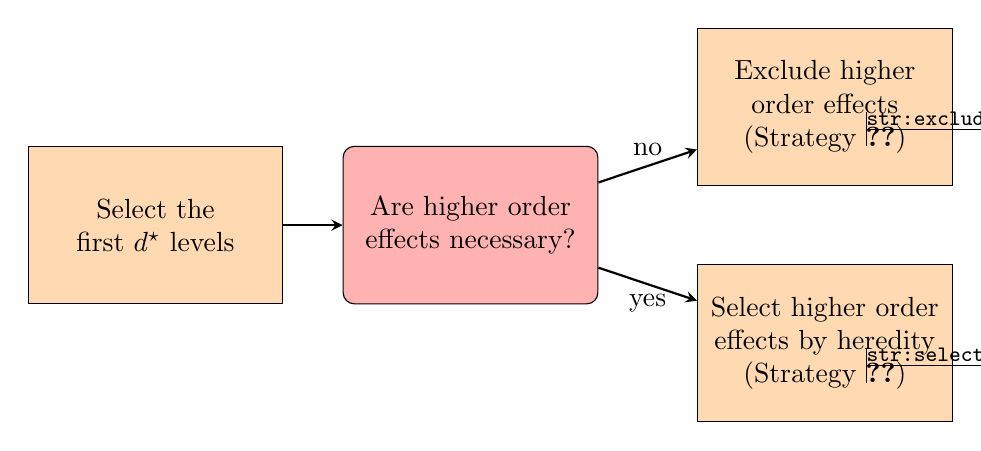
\begin{tikzpicture}[node distance = 2cm]
\node (pro1) [process] {Select the first $d^\star$ levels};
\node (dec2) [startstop, right of=pro1, xshift=2cm] {Are higher order effects necessary? };
\node (pro4) [process, right of=dec2, xshift = 2.5cm, yshift = -1.5cm] {Select higher order effects by heredity (Strategy \ref{str:select-by-heredity})};
\node (pro5) [process, right of=dec2, xshift = 2.5cm,  yshift = 1.5cm] {Exclude higher order effects (Strategy \ref{str:exclude-all})};

\draw [arrow] (pro1) -- (dec2);
\draw [arrow] (dec2) -- node[anchor=north] {yes} (pro4);
\draw [arrow] (dec2) -- node[anchor=south] {no} (pro5);

\end{tikzpicture}
\caption{General strategy for factorial  screening}
\label{fig:general-strategy}
\end{figure}


When using Algorithm \ref{alg:forward-ms}, we can expect that perfect selection is more plausible in the initial levels (say the main effects plus two way interactions), but may cause trouble in the higher order interactions if the higher order interactions are too small in magnitude or the significance level $\alpha_d$ at a particular layer is not well-tuned. Therefore, it is  reasonable to start from the condition that we are only assured perfect selection for the first several levels:
\begin{condition}\label{cond:under-selection}
The selected working model is correct up to the level $d^\star \le D^\star$ with  probability tending to 1:
\begin{align*}
    \Prob{\hat{\bbM}_1 = \bbM^\star_1, \dots, \hat{\bbM}_{d^\star} = \bbM^\star_{d^\star}} \to 1. 
\end{align*}
\end{condition}

Condition \ref{cond:under-selection} does not impose any restriction on the selection results beyond level $d^\star$. In practice we might not have confidence in the selection results beyond $d^\star$, hence we hope to stop before we lose control of the randomness of the selected working model. This motivates the first strategy we want to discuss:

\begin{strategy}[Exclude higher order interactions]\label{str:exclude-all}
 In Algorithm \ref{alg:forward-ms}, set $\alpha_d = \infty,d\ge d^\star + 1$ so that no effects beyond level $d^\star$ will be selected and $\hat{\bbM} = \cup_{d=1}^{d^\star}\hat{\bbM}_{d}$. 
\end{strategy}

Strategy \ref{str:exclude-all} leads to under-selection: $\hat{\bbM}\subset{\bbM}^\star$. In this case, the tricky part for inference is that unbiasedness usually fails for estimating general linear combination of average potential outcomes. To see this, note that
\begin{align}
    \bw^\top \overline{Y} =& \bw^\top G(\cdot,\bbM^\star)\tau(\bbM^\star)\notag \\
    =&  \sum_{d=1}^{d^\star}\bw^\top G(\cdot,\bbM^\star_d)\tau(\bbM^\star_d) + \sum_{d=d^\star+1}^{D^\star} \bw^\top G(\cdot,\bbM^\star_d)\tau(\bbM^\star_d). \label{eqn:decomposition}
\end{align}
Since the selected working model might deviate from the truth beyond level $d^\star$, the second part of \eqref{eqn:decomposition} in general does not have a consistent estimation. Therefore, we will only focus on  coefficient vectors $\bw$ that satisfy certain conditions specified in the following theorem: 

\begin{theorem}[Guarantee for Strategy \ref{str:exclude-all}]\label{thm:strategy-I}
Assume Condition \ref{cond:under-selection}. Also assume $\bw$ satisfies the following orthogonality condition: 
\begin{align}\label{eqn:orthogonality}
    G(\cdot, \bbM_d^{\star})^\top\bw = 0, ~d^\star +1 \le d \le D^\star.
\end{align}
Let $ \tilde{\bw}(\bbM)$ be given by \eqref{eqn:tw} with $\bbM = \cup_{d=1}^{d^\star}\bbM^\star_d$. Assume \eqref{eqn:nondegenerate-var-tw}. 
Then it holds
\begin{align}\label{eqn:tail-under-ms}
    &\sup_{t\in\bbR}\lt|\Prob{\frac{\hgamma(\hat{\bbM})-\gamma}{v(\bbM)} \le t} - \Phi(t)\rt| \notag\\
    &\le 2\Prob{\hat{\bbM}\neq \bbM} +  2C\sigma_w   \frac{\underline{c}^{-1} \max_{i\in[N],\bz\in[Q]}|Y_i(\bz)-\overline{Y}(\bz)|}{\sqrt{\overline{c}^{-1} \min_{\bz\in[Q]} S(\bz,\bz)}\cdot \sqrt{N_0}}\cdot  \frac{\|\tilde{\bw}(\bbM)\|_\infty}{\|\tilde{\bw}(\bbM)\|_2} .
\end{align}
\end{theorem}

Condition \eqref{eqn:orthogonality} states that the coefficient vector $\bw$ should be orthogonal to the higher order contrasts, which makes sense because the under selection procedure cannot provide  screening guarantee for high order interactions. One straightforward example satisfying Condition \eqref{eqn:orthogonality} is linear combination of lower-order contrasts, given by
\begin{align*}
\bw = G(,\cup_{d=1}^{d^\star}\bbM^\star_d) \boldsymbol{b}.
\end{align*}
\inlinemod{red}{more concrete...} Now Condition \eqref{eqn:orthogonality} holds due to the orthogonality between low order and higher order contrasts. 




On the other hand, one might argue that, in certain scenarios people do care about a small number of higher order interactions, for which the  screening procedure cannot work perfectly. In such cases, we propose to select the effects by hierarchy so that higher order effects are included with high interpretability. 


\begin{strategy}[Select higher order interactions by heredity]\label{str:select-by-heredity}
In Algorithm \ref{alg:forward-ms}, set $\alpha_d = 0,d\ge d^\star+1$ and apply a heredity principle (either weak or strong, depending on people's knowledge on the structure of the effects). Then the high order effects beyond level $ d^\star$ are selected merely by heredity principle and 
$$
\hat{\bbM} = \cup_{d=1}^{D}\hat{\bbM}_{d}; ~\hat{\bbM}_{d} = \texttt{\em P}^{(d-d^\star)}(\hat{\bbM}_{d^\star}), d\ge d^\star+1.
$$
Here $\texttt{\em P}^{(d-d^\star)}$ is the $(d-d^\star)$-order composition of $\texttt{\em P}$, meaning applying $\texttt{\em P}$ for $(d-d^\star)$ times.
\end{strategy}


We have the following results for Strategy \ref{str:select-by-heredity}:
\begin{theorem}[Guarantee for Strategy \ref{str:select-by-heredity} ]\label{thm:strategy-II}
Assume Condition \ref{cond:under-selection} and \ref{cond:effects-heredity}. Let 
\begin{align*}
    \bbM^{\star\star} = \bigcup_{d=1}^D \bbM^{\star\star}_d,
\end{align*}
where
\begin{align*}
    \bbM^{\star\star}_d = \left\{
    \begin{array}{cc}
        \bbM^{\star}_d, & d\le d^\star; \\
        \texttt{\em P}^{(d-d^\star)}(\bbM^{\star}_{d^\star}), & d^\star+1\le d\le D.
    \end{array}
    \right.
\end{align*}
Then it holds that
\begin{align*}
    \bbM^\star \subset \bbM^{\star\star},~ \Prob{\hat{\bbM} = \bbM^{\star\star}} \to 1.
\end{align*}
Let $ \tilde{\bw}(\bbM)$ be given by \eqref{eqn:tw} with $\bbM = \bbM^{\star\star} $. Assume \eqref{eqn:nondegenerate-var-tw}. 
Then we have
\begin{align}\label{eqn:tail-over-ms}
    &\sup_{t\in\bbR}\lt|\Prob{\frac{\hgamma(\hat{\bbM})-\gamma}{v(\bbM^{\star\star})} \le t} - \Phi(t)\rt| \notag\\
    &\le 2\Prob{\hat{\bbM}\neq \bbM^{\star\star}} +  2C\sigma_w   \frac{\underline{c}^{-1} \max_{i\in[N],\bz\in[Q]}|Y_i(\bz)-\overline{Y}(\bz)|}{\sqrt{\overline{c}^{-1} \min_{\bz\in[Q]} S(\bz,\bz)}\cdot \sqrt{N_0}}\cdot  \frac{\|\tilde{\bw}(\bbM)\|_\infty}{\|\tilde{\bw}(\bbM)\|_2} .
\end{align}


\end{theorem}


Under Condition \ref{cond:under-selection} and \ref{cond:effects-heredity}, Strategy \ref{str:select-by-heredity} is inherently a particular type of over-selection procedure, since $\hat{\bbM}\subset\bbM^\star$ with high probability. For one thing, Strategy \ref{str:select-by-heredity} can guarantee a good selection result that includes the true model in cases where the higher order interactions are sparse and small in magnitude. For another thing, it preserves the heredity structure in the effects so that the selected working model ensures high interpretability.  

\showproof{\showproofFlag}{
\begin{proof}[Proof of Theorem \ref{thm:strategy-II}]
This proof can be finished by applying Lemma \ref{lem:tail-perfect-ms} with $\bbM=\bbM^{\star\star}$ and checking $\gamma(\bbM^{\star\star}) = \gamma$, which is omitted here. 
\end{proof}
}

When analyzing Strategy \ref{str:exclude-all} and \ref{str:select-by-heredity}, under certain conditions, the selected working model recovers a fixed model with high probability. 

\inlinemod{red}{say more about: (i) under selection - bias-variance trade-off; (ii) over selection: loss of efficiency compared with perfect screening.}

\section{Simulation}

\section{More discussions}

\subsection{Discussion of several  screening methods in finite population factorial experiments}
\begin{itemize}
\item Bonferroni correction:

\item LASSO: {\color{red} soft thresholding!}
\begin{align*}
    \min_{\tau \in \mathbb{R}^H}\sum_{i= 1}^N (y_i - f_i^\top \tau) + \lambda \|\tau\|_1,
\end{align*}

\item AIC: {\color{red} hard thresholding!}
\begin{align*}
    \min_{\tau \in \mathbb{R}^H,\bbM\subset [K]}\sum_{i= 1}^N (y_i - f_i^\top \tau_{\bbM}) + \lambda |\bbM|,
\end{align*}

\item BIC: {\color{red} hard thresholding!}
\begin{align*}
    \min_{\tau \in \mathbb{R}^H, \bbM\subset [K]}\sum_{i= 1}^N (y_i - f_{i,\bbM}^\top \tau_{\bbM}) + \lambda |\bbM| \log(N),
\end{align*}
\end{itemize}

\subsection{Discussion with more general centering values}

\subsubsection{Unsaturated weighted least square: a closed form expression}

In this section we first derive the closed form expression for unsaturated WLS estimation, then verify the nice targeting property we mentioned in the previous section. 

First we need to introduce a transformation matrix $\bP_{\Delta\delta_{[K]}}$, with columns and rows indexed by subsets $\{\cK\subset [K]\}$ of the $K$ factors. Generally it is used to reveal the relationship between designs with different configurations of centering factors $\delta_{[K]}$ and $\delta'_{[K]} = \delta_{[K]}+\Delta\delta_{[K]}$. The transformation is actually linear:
\begin{align}
    \left(f_{\delta'_{[K]}}(z^*_\cK)\right)_{\cK\subset [K]} = \left(f_{\delta_{[K]}}(z^*_\cK)\right)_{\cK\subset [K]} \bP_{\Delta\delta_{[K]}}.
\end{align}

The closed form of $\bP_{\Delta\delta_{[K]}}$ is easy to derive.  Note that for all $\cK'\subset [K]$, we have 
\begin{align}
    f_{\delta'_{[K]}}(z^*_{\cK'}) = \sum_{\cK\subset \cK'}f_{\delta_{[K]}}(z^*_{\cK}) \prod_{k\in \cK'\backslash \cK}(\Delta\delta)_k, \notag
\end{align}
which implies the element of $\bP_{\Delta\delta_{[K]}}$ indexed by $(\cK, \cK')$ is given by
\begin{align}\label{eqn:Pmatrix}
\bP_{\Delta\delta_{[K]}}(\cK,\cK')=\left\{
\begin{array}{ccc}
    \prod_{k\in \cK'\backslash \cK}(\Delta\delta)_k &, & \cK\subset\cK', \\
     0 &, & \cK\subsetneq \cK'. 
\end{array}
\right.
\end{align}

Define $\bQ_{\Delta\delta_{[K]}} = \bP_{\Delta\delta_{[K]}}^{-1}$ to be the inverse. Note that $\bQ_{\Delta\delta_{[K]}}$ is simply taking out a $\Delta\delta_{[K]}$ vector from a group of centering factors, so by symmetry we have 
\begin{align}\label{eqn:Qmatrix}
    \bQ_{\Delta\delta_{[K]}}(\cK,\cK') = \left\{
\begin{array}{ccc}
    (-1)^{|\cK'|-|\cK|}\prod_{k\in \cK'\backslash \cK}(\Delta\delta)_k &, & \cK\subset\cK', \\
     0 &, & \cK\subsetneq \cK'. 
\end{array}
\right.
\end{align}

We shall give an example of the above matrix in the three-factor case, which appears (incompletely) in the appendix of \cite{zhao2021regression}. Let $A'=A-\delta_A$, $B'=B-\delta_B$, $C'=C-\delta_C$. 
\begin{align*}
    \begin{pmatrix}
    1\\
    A\\
    B\\
    C\\
    AB\\
    AC\\
    BC\\
    ABC
    \end{pmatrix} = \bP_{\Delta\delta_{[K]}}^\top 
    \begin{pmatrix}
    1\\
    A'\\
    B'\\
    C'\\
    A'B'\\
    A'C'\\
    B'C'\\
    A'B'C'
    \end{pmatrix}=
    \begin{pmatrix}
    1        & 0 & 0 & 0 & 0 & 0 & 0 & 0 \\
    \delta_A & 1 & 0 & 0 & 0 & 0 & 0 & 0 \\
    \delta_B & 0 & 1 & 0 & 0 & 0 & 0 & 0 \\
    \delta_C & 0 & 0 & 1 & 0 & 0 & 0 & 0 \\
    \delta_A\delta_B & \delta_B & \delta_A & 0 & 1 & 0 & 0 & 0\\ 
    \delta_A\delta_C & \delta_C & 0 & \delta_A & 0 & 1 & 0 & 0\\ 
    \delta_B\delta_C & 0 & \delta_C & \delta_B & 0 & 0 & 1 & 0\\ 
    \delta_A\delta_B\delta_C & \delta_B\delta_C & \delta_A\delta_C & \delta_A\delta_B & \delta_C & \delta_B & \delta_A & 1\\
    \end{pmatrix}
    \begin{pmatrix}
    1\\
    A'\\
    B'\\
    C'\\
    A'B'\\
    A'C'\\
    B'C'\\
    A'B'C'
    \end{pmatrix}.
\end{align*}

The following theorem shows that $\bP_{\Delta\delta_{[K]}}$ and $\bQ_{\Delta\delta_{[K]}}$ totally determines the structure of $\bD_h$.


\begin{theorem}\label{thm:closeD}
Consider weighted least squares with centering factors $\delta_{[K]}$ and weights proportional to size of  each stratum. Let $\Delta\delta_{[K]} = \delta_{[K]}-(1/2)_{k=1}^K$. The unsaturated regression  on up to all $m$-level main/interactions terms has coefficient vector:
\begin{align}\label{eqn:wls-res}
    (\tilde{\tau}_{\cK})_{\{|\cK|\le m\}} = ({\tau}_{\cK})_{\{|\cK|\le m\}} + \bD_h\cdot({\tau}_{\cK})_{\{|\cK|> m\}},
\end{align}
where $\bD_h$ is given by 
\begin{align*}
    \bD_h = \bP_{\Delta\delta_{[K]}}\left(\{\cK\subset [m]\}, \{\cK\subset [m]\}\right) \cdot \bQ_{\Delta\delta_{[K]}}\left(\{\cK\subset [m]\}, \{\cK\subset [K] \backslash[m]\}\right).
\end{align*}
\end{theorem}




\begin{corollary}\label{cor:closeD}
The matrix $\bD$ has a closed form expression:
\begin{enumerate}
    \item For $\cK\subsetneq \cK'$,
    \begin{align}
    \bD_h(\cK, \cK') = 0.
    \end{align}
     
    \item For $\cK\subset \cK'$, let $|\cK|=k$, $|\cK'|=k'$, with $k\le m <k'$,
    \begin{align}
    \bD_h(\cK, \cK') = \sum_{l=0}^{m-k} (-1)^{k'-k+1-l} \begin{pmatrix}
    k'-k+1 \\
    l
    \end{pmatrix}
    \prod_{t\in \cK'\backslash \cK}\left(\delta_t-\frac{1}{2}\right).
    \end{align}
\end{enumerate}

\end{corollary}

\begin{proof}
This result can be derived through careful calculation based on the definition of $\bP$ and $\bQ$ from \eqref{eqn:Pmatrix} and \eqref{eqn:Qmatrix} along with Theorem \ref{thm:closeD} thus omitted here. 
\end{proof}


\subsubsection{A sufficient condition for sign consistency in population WLS regression}

\begin{definition}[Active interaction number]\label{def:sparsity}
For every $z_k$ of the $K$ factors, there are $s_k$ factors that have nonzero interaction with $z_k$, where $s_k\in [K-1]$ is a nonnegative integer associated with $K$. We call $s_k$ the active interaction number of factor $z_k$. The maximal active interaction number is subsequently defined as $s_K = \max_{k\in [K]} s_k$.
\end{definition}

This definition is mainly devoted to finer technical purposes in Theorem \ref{thm:suffcond}. 

\begin{theorem}\label{thm:suffcond}
Assume we run weighted least square under the setting depicted in  Theorem \ref{thm:closeD}. Define the maximal decaying rate $c_K=\max_{l\in[K]} c_l$. Recall the predefined maximal active interaction number $s_K$ from Definition \ref{def:sparsity}. If we have 
\begin{align}
s_Kc_K\max_{k=1,\dots,K} |\delta_k-1/2|<\ln 2, \label{cond:sufficient}
\end{align}
then the unsaturated regression coefficients
$(\tilde{\tau}_{\cK})_{\{|\cK|\le m\}}$ and the corresponding saturated regression coefficients  $({\tau}_{\cK})_{\{|\cK|\le m\}}$ from \eqref{eqn:wls-res} have same signs on every term.

\end{theorem}

Condition \eqref{cond:sufficient} unifies the property of factorial effects and the information of the design pattern(the centering factors $\delta_{[K]}$). The product of $s_K$ and $c_K$ demonstrates a trade-off between the active interaction number and the hierarchy structure. Sparser interactions require slower decaying rate and vice versa. Besides, the product of $s_Kc_K$ and $\max_{k=1,\dots,K} |\delta_k-1/2|$ shows that if $\delta_k$ lies more close to $1/2$, less restriction are needed on the effect structure. This aligns with the result in \cite{zhao2021regression}: when $\delta_k=1/2$ holds for all $k=1,\dots, K$,  $\bD_h=\boldsymbol{0}$, so that forward selection always works. 

\section{Simulation}



\section{Conclusion}

\bibliographystyle{apalike}
\bibliography{ref.bib}

\appendix

\section{Technical proofs}
\subsection{Preliminaries: some important probabilistic results in randomized experiments}

Consider an estimator of the form
\begin{align*}
    \hgamma = Q^{-1}\sum_{\bz\in\cT} w(\bz)\hat{Y}(\bz),
\end{align*}
with variance estimation
\begin{align*}
    \hat{v}^2_R = Q^{-2}\sum_{\bz\in\cT} w(\bz)^2 \hat{S}(\bz,\bz).
\end{align*}

We have the following variance estimation results and Berry-Esseen bounds:

\begin{lemma}[Variance concentration and Berry-Esseen bounds in finite population]\label{lem:BE-finite-pop}
Denote $\gamma = \bbE\{\hgamma\}$, $v^2 = \operatorname{Var}(\hgamma)$ and $v^2_R = \bbE\{\hat{v}^2_R\}$.
Suppose the following conditions hold: 
\begin{itemize}
    \item  Nondegenerate variance. There exists a $\sigma_w > 0$, such that
    \begin{align}\label{eqn:nondegenerate-var}
        Q^{-2}\sum_{\bz=1}^Q w(\bz)^2 N_{\bz}^{-1} S(\bz,\bz) \le \sigma_w^2 v^2.
    \end{align}
    
    \item Bounded fourth moments. There exists a $ \delta > 0$ such that
    \begin{align}\label{eqn:bounded-moments}
    \max_{\bz\in[Q]}\frac{1}{N}\sum_{i=1}^N \{Y_i(\bz) - \overline{Y}(\bz)\}^4 \le \Delta^4.
    \end{align}
\end{itemize}


\begin{enumerate}
    \item The variance estimator is robust for the true variance:
    $v_R \ge v$. Besides, the following tail bound holds:
    \begin{align}\label{eqn:tail-vhatR}
        \bbP\lt\{N |\hat{v}_R-v_R | > t\rt\} 
        \le \frac{C\overline{c}^3\underline{c}^{-4} \|w\|_\infty^2 \Delta^4 }{QN_0}\cdot \frac{1}{t^2}.
    \end{align}

    \item We have a Berry-Esseen bound with the true variance:
    \begin{align}\label{eqn:uniform-design-be}
       \sup_{t\in\bbR}\lt|\Prob{\frac{\hgamma-\gamma}{v} \le t} - \Phi(t)\rt|  \le  2C\sigma_w   \frac{\underline{c}^{-1}  \|w\|_{\infty}   \max_{i\in[N],\bz\in[Q]}|Y_i(\bz)-\overline{Y}(\bz)|}{\|w\|_2\sqrt{\overline{c}^{-1} \min_{\bz\in[Q]} S(\bz,\bz)}\cdot \sqrt{ N_0}} .
    \end{align}
    
    \item We have a Berry-Esseen bound with the estimated variance: for any $\epsilon_N \in (0, 1/2]$,
    \begin{align*}
        \sup_{t\in\bbR}\lt|\bbP\lt\{\frac{\hgamma - \gamma}{\hat{v}_R} \le t\rt\} - \Phi\lt(\frac{v_R}{v}t\rt)\rt| &\le
        \epsilon_N +  \frac{C\overline{c}^3\underline{c}^{-4} \|w\|_\infty^2 \Delta^4 }{QN_0}\cdot \frac{1}{(Nv^2\epsilon_N)^2} \\
        &+ 2C\sigma_w   \frac{\underline{c}^{-1}  \|w\|_{\infty}   \max_{i\in[N],\bz\in[Q]}|Y_i(\bz)-\overline{Y}(\bz)|}{\|w\|_2\sqrt{\overline{c}^{-1} \min_{\bz\in[Q]} S(\bz,\bz)}\cdot \sqrt{N_0}}.
    \end{align*}
\end{enumerate}

\end{lemma}

\showproof{\showproofFlag}{
\begin{proof}[Proof of Lemma \ref{lem:BE-finite-pop}]
\begin{enumerate}
    \item {\color{red} BE-PCLT Corollary 2}.

    \item {\color{red} BE-PCLT Theorem 8}.
    
    \item Proof of the third part. First we show a useful result: for $|a|\le 1/2$ and any $b\in\bbR$, 
    \begin{align}\label{form:Phi-bD}
        \sup_{t\in\bbR}|\Phi\{(1+a)t + b\} - \Phi\{t\}| \le |a| + |b|.
    \end{align}
    This can be proved by a simple step of intermediate value theorem: for any $t\in\bbR$,
    \begin{align*}
        &|\Phi\{(1+a)t + b\} - \Phi\{t\}| \\
        =& |\phi(\xi_{t,(1+a)t})\cdot (at + b)|\\
        =& |\phi(\xi_{t,(1+a)t})\cdot at| + |\phi(\xi_{t,(1+a)t})\cdot b|\\
        =& |a| \cdot |\phi(\xi_{t,(1+a)t})\cdot t|\cdot \ind{|t|\le 1} + |a| \cdot |\phi(\xi_{t,(1+a)t})\cdot t|\cdot \ind{|t| > 1} + |\phi(\xi_{t,(1+a)t})\cdot b|\\
        \le& \frac{1}{\sqrt{2\pi}}|a|\cdot \ind{|t|\le 1} + \frac{1}{\sqrt{2\pi}} |a| |t|\cdot\exp(-t^2/8)\cdot\ind{|t| > 1} +  {\frac{1}{\sqrt{2\pi}}}|b|\\
        \le& |a| + |b|.
    \end{align*}
    WLOG we consider $t\ge 0$ since $t<0$ can be handled similarly. For any $\epsilon_N > 0$, We have
    \begin{align*}
        \bbP\lt\{\frac{\hgamma - \gamma}{\hat{v}_R} \le t\rt\} &= \bbP\lt\{\frac{\hgamma - \gamma}{{v}} \le \frac{\hat{v}_R}{{v}}t\rt\}\\
        &= \bbP\lt\{\frac{\hgamma - \gamma}{{v}} \le \frac{\hat{v}_R}{{v}}t, \lt|\frac{\hat{v}_R - v_R}{v}\rt| \le \epsilon_N\rt\} + \bbP\lt\{\frac{\hgamma - \gamma}{{v}} \le \frac{\hat{v}_R}{{v}}t, \lt|\frac{\hat{v}_R - v_R}{v}\rt| > \epsilon_N\rt\}.
    \end{align*}
    Then we can show that
    \begin{align*}
        \bbP\lt\{\frac{\hgamma - \gamma}{\hat{v}_R} \le t\rt\} &\le 
        \bbP\lt\{\frac{\hgamma - \gamma}{{v}} \le \frac{\hat{v}_R}{{v}}t, \lt|\frac{\hat{v}_R - v_R}{v}\rt| \le \epsilon_N\rt\} + \bbP\lt\{ \lt|\frac{\hat{v}_R - v_R}{v}\rt| > \epsilon_N\rt\}\\
        &\le \bbP\lt\{\frac{\hgamma - \gamma}{{v}} \le \lt(\frac{{v}_R}{v} + \epsilon_N\rt)t\rt\} + \bbP\lt\{ \lt|\frac{\hat{v}_R - v_R}{v}\rt| > \epsilon_N\rt\}.
    \end{align*}
    
    For the first term, we have
    \begin{align*}
        &\sup_{t\ge 0}\lt|\bbP\lt\{\frac{\hgamma - \gamma}{{v}}   \le \lt(\frac{{v}_R}{v} + \epsilon_N\rt)t\rt\} - \Phi\lt\{\lt(\frac{{v}_R}{v} + \epsilon_N\rt)t \rt\}\rt| \\
        &\le 2C\sigma_w   \frac{\underline{c}^{-1}  \|w\|_{\infty}   \max_{i\in[N],\bz\in[Q]}|Y_i(\bz)-\overline{Y}(\bz)|}{\|w\|_2\sqrt{\overline{c}^{-1} \min_{\bz\in[Q]} S(\bz,\bz)}\cdot \sqrt{ N_0}}.
    \end{align*}
    For the second term, using the variance estimation results in Part 1 we have
    \begin{align*}
        \bbP\lt\{ \lt|\frac{\hat{v}_R - v_R}{v}\rt| \ge \epsilon_N\rt\} &\le  \bbP\lt\{ \lt|\frac{\hat{v}_R - v_R}{v}\rt|\cdot\lt|\frac{\hat{v}_R + v_R}{v}\rt| \ge \epsilon_N\rt\} \see{since $v_R$ is robust}\\
        & =  \bbP\lt\{ \lt|\frac{N\hat{v}^2_R - Nv^2_R}{Nv^2}\rt| \ge \epsilon_N\rt\}   \\
        & \le \frac{C\overline{c}^3\underline{c}^{-4} \|w\|_\infty^2 \Delta^4 }{QN_0}\cdot \frac{1}{(Nv^2\epsilon_N)^2}.
    \end{align*}
    Besides, by \eqref{form:Phi-bD}, when $\epsilon_N\le 1/2$, we also have
    \begin{align*}
        \sup_{t\in\bbR}\lt|\Phi\lt\{\lt(\frac{{v}_R}{v} + \epsilon_N \rt)t \rt\} - \Phi\lt(\frac{v_R}{v}t\rt)\rt| \le \frac{v\epsilon_N}{v_R} \le \epsilon_N. 
    \end{align*}
    Aggregating all the parts above, we can show that for any $t\ge 0$,
    \begin{align*}
        \bbP\lt\{\frac{\hgamma - \gamma}{\hat{v}_R} \le t\rt\} &\le \Phi\lt(\frac{v_R}{v}t\rt) + \epsilon_N +  \frac{C\overline{c}^3\underline{c}^{-4} \|w\|_\infty^2 \Delta^4 }{QN_0}\cdot \frac{1}{(Nv^2\epsilon_N)^2} \\
        &+ 2C\sigma_w   \frac{\underline{c}^{-1}  \|w\|_{\infty}   \max_{i\in[N],\bz\in[Q]}|Y_i(\bz)-\overline{Y}(\bz)|}{\|w\|_2\sqrt{\overline{c}^{-1} \min_{\bz\in[Q]} S(\bz,\bz)}\cdot \sqrt{N_0}}.
    \end{align*}
    
    On the other hand, we can show that
    \begin{align}
        \bbP\lt\{\frac{\hgamma - \gamma}{\hat{v}_R} \le t\rt\} &\ge 
        \bbP\lt\{\frac{\hgamma - \gamma}{{v}} \le \frac{\hat{v}_R}{{v}}t, \lt|\frac{\hat{v}_R - v_R}{v}\rt| \le \epsilon_N\rt\} \notag\\
        &\ge \bbP\lt\{\frac{\hgamma - \gamma}{{v}} \le \lt(\frac{{v}_R}{v} - \epsilon_N\rt)t\rt\} - \bbP\lt\{ \lt|\frac{\hat{v}_R - v_R}{v}\rt| \ge \epsilon_N\rt\}.\label{eqn:upper-bd}
    \end{align}
    By \eqref{form:Phi-bD}, when $\epsilon_N\le 1/2$, we also have
    \begin{align*}
        \sup_{t\in\bbR}\lt|\Phi\lt\{\lt(\frac{{v}_R}{v} - \epsilon_N\rt)t \rt\} - \Phi\lt(\frac{v_R}{v}t\rt)\rt| \le \epsilon_N. 
    \end{align*}
    So we can derive a lower bound analogous to \eqref{eqn:upper-bd}. Note that the results can be analogously generalized to $t\le 0$. Putting pieces together, we can show that for any $t\ge 0$,
    \begin{align*}
        \sup_{t\in\bbR}\lt|\bbP\lt\{\frac{\hgamma - \gamma}{\hat{v}_R} \le t\rt\} - \Phi\lt(\frac{v_R}{v}t\rt)\rt| &\le
        \epsilon_N +  \frac{C\overline{c}^3\underline{c}^{-4} \|w\|_\infty^2 \Delta^4 }{QN_0}\cdot \frac{1}{(Nv^2\epsilon_N)^2} \\
        &+ 2C\sigma_w   \frac{\underline{c}^{-1}  \|w\|_{\infty}   \max_{i\in[N],\bz\in[Q]}|Y_i(\bz)-\overline{Y}(\bz)|}{\|w\|_2\sqrt{\overline{c}^{-1} \min_{\bz\in[Q]} S(\bz,\bz)}\cdot \sqrt{ N_0}}.
    \end{align*}
\end{enumerate}


\end{proof}
}

The following corollary shows the studentized Berry-Esseen bounds in the special case where $w = (w(\bz))_{\bz\in[Q]}$ is a contrast vector for factorial effects. That is, $ w = g_\cK$ for some $\cK \in \bbK $. 

\begin{corollary}\label{cor:factorial-student-be}
Assume Condition \eqref{eqn:nondegenerate-var} and \eqref{eqn:bounded-moments} hold. Let $ w = g_\cK$ for some $\cK \in \bbK $. Then we have a Berry-Esseen bound with the estimated variance:
\begin{align*}
    \sup_{t\in\bbR}\lt|\bbP\lt\{\frac{\htau_\cK - \tau_\cK}{\hat{v}_R} \le t\rt\} - \Phi\lt(\frac{v_R}{v}t\rt)\rt| &\le
          2\lt(\frac{C\sigma_w^4\overline{c}^5\underline{c}^{-6}  \Delta^4 }{\{\min_{\bz\in\cT}S(\bz,\bz)\}^2}\rt)^{1/3}\cdot\frac{1}{(QN_0)^{1/3}} \\
        &+ 2C\sigma_w   \frac{\underline{c}^{-1}     \max_{i\in[N],\bz\in[Q]}|Y_i(\bz)-\overline{Y}(\bz)|}{ \sqrt{\overline{c}^{-1} \min_{\bz\in[Q]} S(\bz,\bz)}}\cdot\frac{1}{(QN_0)^{1/2}}.
\end{align*}
\end{corollary}

\showproof{\showproofFlag}{
\begin{proof}[Proof of Corollary \ref{cor:factorial-student-be}]
\textbf{Lower bound for $Nv^2$.} Note that
$\|w\|_2^2 = Q, \|w\|_\infty = 1$. 
Using Condition \eqref{eqn:nondegenerate-var}, we have
\begin{align*}
    Nv^2 &\ge N\sigma_w^{-2} Q^{-2}\sum_{\bz=1}^Q w(\bz)^2 N_{\bz}^{-1} S(\bz,\bz) \\
    &\ge (\underline{c}QN_0)\cdot\sigma_w^{-2} \overline{c}^{-1}Q^{-1}N_{0}^{-1} \min_{\bz\in\cT} S(\bz,\bz) \cdot (Q^{-1}\|w\|_2^2)\\
    &= \sigma_w^{-2}\underline{c}\overline{c}^{-1}\min_{\bz\in\cT}S(\bz,\bz).
\end{align*}

Therefore, the Berry-Esseen bound becomes
\begin{align*}
    \sup_{t\in\bbR}\lt|\bbP\lt\{\frac{\htau_\cK - \tau_\cK}{\hat{v}_R} \le t\rt\} - \Phi\lt(\frac{v_R}{v}t\rt)\rt| &\le
        \epsilon_N +  \frac{C\sigma_w^4\overline{c}^5\underline{c}^{-6}  \Delta^4 }{(QN_0)\{\min_{\bz\in\cT}S(\bz,\bz)\}^2}\cdot \frac{1}{\epsilon_N^2} \\
        &+ 2C\sigma_w   \frac{\underline{c}^{-1}     \max_{i\in[N],\bz\in[Q]}|Y_i(\bz)-\overline{Y}(\bz)|}{\sqrt{\overline{c}^{-1} \min_{\bz\in[Q]} S(\bz,\bz)}\cdot \sqrt{QN_0}}.
\end{align*}

\textbf{Optimize the summation of the first and second term.}
By taking derivative over $\epsilon_N $ on the upper bound and solving for the zero point, we know that when 
\begin{align*}
    \epsilon_N = \lt(\frac{2C\sigma_w^4\overline{c}^5\underline{c}^{-6}  \Delta^4 }{(QN_0)\{\min_{\bz\in\cT}S(\bz,\bz)\}^2}\rt)^{1/3},
\end{align*}
the upper bound is minimized and 
\begin{align*}
    \sup_{t\in\bbR}\lt|\bbP\lt\{\frac{\htau_\cK - \tau_\cK}{\hat{v}_R} \le t\rt\} - \Phi\lt(\frac{v_R}{v}t\rt)\rt| &\le
          2\lt(\frac{C\sigma_w^4\overline{c}^5\underline{c}^{-6}  \Delta^4 }{\{\min_{\bz\in\cT}S(\bz,\bz)\}^2}\rt)^{1/3}\cdot\frac{1}{(QN_0)^{1/3}} \\
        &+ 2C\sigma_w   \frac{\underline{c}^{-1}     \max_{i\in[N],\bz\in[Q]}|Y_i(\bz)-\overline{Y}(\bz)|}{ \sqrt{\overline{c}^{-1} \min_{\bz\in[Q]} S(\bz,\bz)}}\cdot\frac{1}{(QN_0)^{1/2}}.
\end{align*}
\end{proof}
}

Additionally, we have a Berry-Esseen bounds after screening the effects:

\begin{lemma}[Berry Esseen bound with  screening]\label{lem:tail-perfect-ms} Let 
\begin{align}\label{eqn:tw}
\tilde{\bw}_{\bbM} = Q^{-1}G(\cdot,\bbM)G(\cdot,\bbM)^\top\bw.
\end{align}
Assume there exists $\sigma_w>0$ such that
\begin{align}\label{eqn:nondegenerate-var-tw}
    \sum_{\bz=1}^Q \tilde{\bw}_{\bbM}(\bz)^2 N_{\bz}^{-1} S(\bz,\bz) \le \sigma_w^2 v^2(\bbM).
\end{align}
Then it holds
\begin{align}\label{eqn:tail-perfect-ms}
    &\sup_{t\in\bbR}\lt|\Prob{\frac{\hgamma(\hat{\bbM})-\gamma(\bbM)}{v(\bbM)} \le t} - \Phi(t)\rt| \notag\\
    &\le 2\Prob{\hat{\bbM}\neq \bbM} +  2C\sigma_w   \frac{\underline{c}^{-1} \max_{i\in[N],\bz\in[Q]}|Y_i(\bz)-\overline{Y}(\bz)|}{\sqrt{\overline{c}^{-1} \min_{\bz\in[Q]} S(\bz,\bz)}\cdot \sqrt{N_0}}\cdot  \frac{\|\tilde{\bw}_{\bbM}\|_\infty}{\|\tilde{\bw}_{\bbM}\|_2} .
\end{align}
\end{lemma}


{
\begin{proof}[Proof of Lemma \ref{lem:tail-perfect-ms}]
With the selected working model we have
\begin{align*}
    &\sup_{t\in\bbR}\lt|\Prob{\frac{\hgamma(\hat{\bbM})-\gamma(\bbM)}{v(\bbM)} \le t} - \Phi(t)\rt| \\
    = &\sup_{t\in\bbR}\lt|\Prob{\frac{\hgamma(\hat{\bbM})-\gamma(\bbM)}{v(\bbM)} \le t, \hat{\bbM} = \bbM} - \Phi(t) + \Prob{\frac{\hgamma(\hat{\bbM})-\gamma(\bbM)}{v(\bbM)} \le t, \hat{\bbM} \neq \bbM} \rt|\\
    \le &\sup_{t\in\bbR}\lt|\Prob{\frac{\hgamma(\hat{\bbM})-\gamma(\bbM)}{v(\bbM)} \le t, \hat{\bbM} = \bbM} - \Phi(t)\rt| +  \Prob{\frac{\hgamma(\hat{\bbM})-\gamma(\bbM)}{v(\bbM)} \le t, \hat{\bbM} \neq \bbM}  \\
    = &\sup_{t\in\bbR}\lt|\Prob{\frac{\hgamma({\bbM})-\gamma(\bbM)}{v(\bbM)} \le t, \hat{\bbM} = \bbM} - \Phi(t)\rt| +  \Prob{\frac{\hgamma(\hat{\bbM})-\gamma(\bbM)}{v(\bbM)} \le t, \hat{\bbM} \neq \bbM}  \\
    \le & \sup_{t\in\bbR}\lt|\Prob{\frac{\hgamma({\bbM})-\gamma(\bbM)}{v(\bbM)} \le t} - \Phi(t)\rt| +  2\Prob{ \hat{\bbM} \neq \bbM}.
\end{align*}

Now we have 
\begin{align*}
    \hgamma(\bbM) &= \bw^\top G(\cdot, \bbM) \htau(\bbM) \\
    & =  \bw^\top G(\cdot, \bbM) G(\cdot, \bbM)^\top \hY \\
    & = \tilde{\bw}_{\bbM}^\top \hY.
\end{align*}


By \inlinemod{red}{Corollary 2 of BE-PCLT},  we have a Berry-Esseen bound with the true variance:
\begin{align*}
    \sup_{t\in\bbR}\lt|\Prob{\frac{\hgamma( {\bbM})-\gamma(\bbM)}{v} \le t} - \Phi(t)\rt| 
    \le  2C\sigma_w   \frac{\|\tilde{\bw}_{\bbM}\|_\infty\underline{c}^{-1} \max_{i\in[N],\bz\in[Q]}|Y_i(\bz)-\overline{Y}(\bz)|}{\|\tilde{\bw}_{\bbM} \|_2\sqrt{\overline{c}^{-1} \min_{\bz\in[Q]} S(\bz,\bz)}\cdot \sqrt{ N_0}}.  
\end{align*}
    
\end{proof}
}



\subsection{Proof of Theorem \ref{thm:ms-consistency}}
{
\begin{proof}[Proof of Theorem \ref{thm:ms-consistency}]
\textbf{Induction proof of a basic fact.} According to the orthogonality of designs, the signs for all terms in the studied unsaturated population regressions are consistent with those of saturated regressions, which saves the effort of differentiating true models for partial and full regression. By induction we hope to prove the following fact under the given assumptions:


\begin{displayquote}
For all $D_0\le D$, we have 
\begin{align}\label{eqn:zerofn-general}
\lt|\bbP\lt(\hat{\bbM}_d\subset\bbM^\star_d, d=1,\cdots,D_0\rt)-\bbP\lt(\hat{\bbM}_d=\bbM^\star_d, d=1,\cdots,D_0\rt)\rt|\to 0.
\end{align} 
\end{displayquote}

Because for any $D_0\in[D]$, we always have:
$$\lt\{\hat{\bbM}_d=\bbM^\star_d, d=1,\cdots,D_0\rt\}\subset\lt\{\hat{\bbM}_d\subset\bbM^\star_d, d=1,\cdots,D_0\rt\},$$ 
\eqref{eqn:zerofn-general} is equivalent to: for all $D_0\le D$,
\begin{align}\label{eqn:zerofn-general-1}
\bbP\lt(\text{for all } d\in[D_0],\hat{\bbM}_d\subset\bbM^\star_d; \text{ there exists } d\in[D_0], \hat{\bbM}_d\subsetneq\bbM^\star_d\rt)\to 0.
\end{align} 


\begin{enumerate}
    \item \textbf{Main effects.}
    First, since we assume the tests are consistent (Assumption \ref{asp:valid-consistent}), meaning asymptotically no false negatives:
    \begin{align*}
        \bbP\left({\hat{\bbM}_1}^c \cap\bbM^\star_1\neq \varnothing\right)\to 0 \Leftrightarrow \bbP\left(\bbM^\star_1\subset{\hat{\bbM}_1}\right)\to 1.
    \end{align*}
     
    Therefore,
    \begin{align}\label{eqn:zerofn-general-2}
      \bbP\lt(\hat{\bbM}_1\subsetneq\bbM^\star_1\rt)\to 0. \see{no under selection for main effects}
    \end{align} 
    
    
    
    \item \textbf{Induction validity.}
    Generally speaking, the induction proceeds based on the following idea:
    

    
    The case for $D_0=1$ has been shown in the previous part. Now assume \eqref{eqn:zerofn-general} or \eqref{eqn:zerofn-general-1} for some $D_0\ge1$.  For $D_0+1$, 
    the following holds:
    \begin{align*} 
        0&\le \bbP\left(\left\{\hat{\bbM}_d\subset\bbM^\star_d, d\le D_0+1\right\}\right)-\bbP\left(\left\{\hat{\bbM}_d=\bbM^\star_d, d\le D_0; \hat{\bbM}_{D_0+1}\subset\bbM^\star_{D_0+1}\right\}\right) \\
        &= \bbP\left(\left\{\hat{\bbM}_d\subset\bbM^\star_d, d\le D_0+1\right\} - \left\{\hat{\bbM}_d=\bbM^\star_d, d\le D_0; \hat{\bbM}_{D_0+1}\subset\bbM^\star_{D_0+1}\right\}\right)\notag\\
        &\le \bbP\left(\forall d\in[D_0+1], \hat{\bbM}_{d}\subset\bbM^\star_{d}; \exists d\in[D_0], \hat{\bbM}_d\subsetneq\bbM^\star_d\right)\notag\\
        &\le \bbP\left(\forall d\in[D_0], \hat{\bbM}_{d}\subset\bbM^\star_{d};\exists d\in[D_0], \hat{\bbM}_d\subsetneq\bbM^\star_d\right)\to 0.\see{by \eqref{eqn:zerofn-general-1}}
    \end{align*}
    Hence
    \begin{align}\label{eqn:zerofun-general-2}
        \lt|\bbP\left(\left\{\hat{\bbM}_d\subset\bbM^\star_d, d\le D_0+1\right\}\right) - 
        \bbP\left(\left\{\hat{\bbM}_d=\bbM^\star_d, d\le D_0; \hat{\bbM}_{D_0+1}\subset\bbM^\star_{D_0+1}\right\}\right)\rt| \to 0.
    \end{align}
    
    Now $\hat{\bbM}_{D_0+1}$ is generated based on $\hat{\bbM}_{D_0}$ and the set of estimates over the prescreened effect set  $\hat{\bbM}_{D_0+1,+}$. Under Assumption \ref{asp:P-heredity}, on the event $\hat{\bbM}_d = \bbM_d^\star$ we have
    \begin{align*}
        \hat{\bbM}_{d+1} = \tilde{\bbM}_{d+1}.
    \end{align*}
    
    Hence we can compute
    \begin{align*}
        0\le& \bbP\left(\lt\{\hat{\bbM}_d=\bbM^\star_d, d\le D_0; \hat{\bbM}_{D_0+1}\subset\bbM^\star_{D_0+1}\rt\}\right) - \bbP\left(\hat{\bbM}_d=\bbM^\star_d, d\le D_0+1\right)\\
        = & \bbP\left(\hat{\bbM}_d=\bbM^\star_d, d\le D_0; \hat{\bbM}_{D_0+1}\subsetneq \bbM^{\star }_{D_0+1}\right) \\
        = & \bbP\left(\hat{\bbM}_d=\bbM^\star_d, d\le D_0; \tilde{\bbM}_{D_0+1}\subsetneq \bbM^{\star }_{D_0+1}\right) \\
        \le&  \bbP\left(\tilde{\bbM}^c_{D_0+1}\cap\bbM^{\star }_{D_0+1}\neq\varnothing\right)\to 0.
    \end{align*}
   The last convergence holds  because of the consistency of the test.
    
    The induction can be proceeded. 
    
    
    \textbf{Proof of the first result.} Now it follows
    \begingroup
    \allowdisplaybreaks
    \begin{align}
    &\underset{N\to\infty}{\lim\sup}~\bbP\left(\hat{\bbM}_d\cap{(\bbM^\star_d)}^c\neq\varnothing \text{ for some }d\in[D]\right) \notag\\
    &= 
    \underset{N \to\infty}{\lim\sup}~\bbP\left(\hat{\bbM}_1\cap{\bbM_1^\star}^c\neq\varnothing\right) + \sum_{D_0=2}^{D} \bbP\left(\hat{\bbM}_d\cap{\bbM_d^\star}^c=\varnothing,d=1,\cdots,D_0-1; \hat{\bbM}_{D_0}\cap \bbM_{D_0}^{\star c}\neq\varnothing\right)\notag\\
    &=
    \underset{N \to\infty}{\lim\sup}~\bbP\left(\hat{\bbM}_1\cap{\bbM_1^\star}^c\neq\varnothing\right) + \sum_{D_0=2}^D \bbP\left( \hat{\bbM}_d=\bbM^\star_d,d=1,\cdots,D_0-1; \hat{\bbM}_{D_0}\cap{\bbM_{D_0}^{\star c}}\neq\varnothing\right) \notag\\
    &\see{using \eqref{eqn:zerofn-general} and the fact that $D$ is a fixed integer}\notag\\
    &\le \underset{N \to\infty}{\lim\sup}~\bbP\left(\hat{\bbM}_1\cap{\bbM_1^\star}^c\neq\varnothing\right) + \sum_{D_0=2}^D \bbP\left( \hat{\bbM}_d=\bbM^\star_d,d=1,\cdots,D_0-1; \tilde{\bbM}_{D_0}\cap\bbM_{D_0}^{\star c}\neq\varnothing\right)  \notag\\
    &\see{on the given event, $\hat{\bbM}_{D_0,+} = \cP(\hat{\bbM}_{D_0-1}) = \cP({\bbM}^\star_{D_0-1}) = {\bbM}^\star_{D_0,+}$ and $\hat{\bbM}_{D_0} = \cS_N(\hat{\bbM}_{D_0,+}) = \tilde{\bbM}_{D_0}$}\notag\\
    &\le \underset{N \to\infty}{\lim\sup}~\bbP\left(\hat{\bbM}_1\cap{\bbM_1^\star}^c\neq\varnothing\right) + \sum_{D_0=2}^D \bbP\left(  \tilde{\bbM}_{D_0}\cap{\bbM_{D_0}^\star}^c\neq\varnothing\right)
    \le \sum_{D_0=1}^D\alpha_{D_0} = \alpha. \label{eqn:fwer-general}
\end{align}
\endgroup
Therefore the target probability gets controlled under $\alpha$.

\textbf{Proof of the second result.} Under $\alpha=\alpha_N\to0$, \eqref{eqn:fwer-general} implies that with probability tending to one, 
{
\color{blue} 
\[
\hat{\bbM}_d\cap(\bbM^\star_d)^c = \varnothing,  \text{ for } d=1,\cdots, D \Leftrightarrow \hat{\bbM}_d\subset \bbM^\star_d = \varnothing,  \text{ for } d=1,\cdots, D.
\]
(hope this time it is easier to read?)
}
Now apply \eqref{eqn:zerofn-general}, we obtain
\[
\hat{\bbM}_d=\bbM^\star_d,  \text{ for } d=1,\cdots, D,
\]
with probability tending to one, which concludes the proof.

\end{enumerate}

\end{proof}
}



\subsection{Proof of Corollary \ref{cor:marginal-t}}
{
\begin{proof}[Proof of Corollary \ref{cor:marginal-t}]
\begin{enumerate}
    \item First, we show validity:
    \begin{align*}
        \underset{N\to\infty}{\lim\sup}~\bbP\lt\{\tilde{\bbM}_{d}\cap\bbM^{\star c}_d\neq \varnothing\rt\} 
        &= \underset{N\to\infty}{\lim\sup}~\bbP\lt\{\exists \cK\in\bbM^{\star }_{d,+}\backslash\bbM^{\star }_{d}, \lt|\frac{\htau_{\cK}}{\hat{\sigma}_\cK}\rt|\ge\Phi^{-1}\lt(1-\frac{\alpha_d}{2|\bbM^{\star }_{d,+}|} \rt)\rt\}\\
        &\le\underset{N\to\infty}{\lim\sup}~ \sum_{\cK\in\bbM^{\star }_{d,+}\backslash\bbM^{\star }_{d}} \bbP\lt\{\lt|\frac{\htau_{\cK}}{\hat{\sigma}_\cK}\rt|\ge\Phi^{-1}\lt(1-\frac{\alpha_d}{2|\bbM^{\star }_{d,+}|} \rt)\rt\}\\
        &\le \underset{N\to\infty}{\lim\sup}\sum_{\cK\in\bbM^{\star }_{d,+}\backslash\bbM^{\star }_{d}} ~\lt(\frac{\alpha_d}{|\bbM^{\star }_{d,+}|} + \frac{\tilde{C}}{(QN_0)^{1/3}}\rt)
         \\
        &\le \alpha_d.
    \end{align*}
    \item Second, we show consistency.
    \begin{align*}
        &\underset{N\to\infty}{\lim\sup}~\bbP\lt\{\tilde{\bbM}^c_{d}\cap\bbM^{\star }_d\neq \varnothing\rt\} \\
        &= \underset{N\to\infty}{\lim\sup}~\bbP\lt\{\exists \cK\in \bbM^{\star }_{d}, \lt|\frac{\htau_{\cK}}{\hat{\sigma}_\cK}\rt|\le\Phi^{-1}\lt(1-\frac{\alpha_d}{2|\bbM^{\star }_{d,+}|} \rt)\rt\}\\
        &\le \underset{N\to\infty}{\lim\sup}~ \sum_{\cK\in\bbM^{\star }_{d}} \bbP\lt\{\lt|\frac{\htau_{\cK}}{\hat{\sigma}_\cK}\rt|\le\Phi^{-1}\lt(1-\frac{\alpha_d}{2|\bbM^{\star }_{d,+}|} \rt)\rt\}\\
        &\le \underset{N\to\infty}{\lim\sup}~ \sum_{\cK\in\bbM^{\star }_{d}} \bbP\lt\{\lt|\frac{\htau_{\cK}}{ {\sigma}_\cK}\rt|\le\frac{\hat{\sigma}_\cK}{\sigma_\cK}\Phi^{-1}\lt(1-\frac{\alpha_d}{2|\bbM^{\star }_{d,+}|} \rt)\rt\}\\
        &\le \underset{N\to\infty}{\lim\sup}~ \sum_{\cK\in\bbM^{\star }_{d}} \bbP\lt\{\lt|\frac{\htau_{\cK}}{ {\sigma}_\cK}\rt|\le\lt\{1+\frac{\tilde{C}}{(QN_0)^{1/3}}\rt\}\Phi^{-1}\lt(1-\frac{\alpha_d}{2|\bbM^{\star }_{d,+}|} \rt)\rt\} + \Prob{\frac{\hat{\sigma}_\cK}{\sigma_\cK}> 1+\frac{\tilde{C}}{(QN_0)^{1/3}}}.
    \end{align*}
    For simplicity, let
    \begin{align*}
        Z_d^\star = \Phi^{-1}\lt(1-\frac{\alpha_d}{2|\bbM^{\star }_{d,+}|} \rt). 
    \end{align*}
    Then
    \begin{align}
        &\underset{N\to\infty}{\lim\sup}~\bbP\lt\{\tilde{\bbM}^c_{d}\cap\bbM^{\star }_k\neq \varnothing\rt\} \notag\\
        &\le \underset{N\to\infty}{\lim\sup}~ \sum_{\cK\in\bbM^{\star }_{d}} \lt(\bbP\lt\{-Z_d^\star - \frac{\tau_\cK}{\sigma_\cK}\le\frac{\htau_{\cK}}{ {\sigma}_\cK} - \frac{\tau_\cK}{\sigma_\cK}\le Z_d^\star - \frac{\tau_\cK}{\sigma_\cK}\rt\} + \frac{\tilde{C}}{(QN_0)^{1/3}}\rt)\notag\\
        & = \underset{N\to\infty}{\lim\sup}~\sum_{\cK\in\bbM_d^\star} \Phi\lt\{r_\cK^{-1}\lt(Z_d^\star - \frac{\tau_\cK}{\sigma_\cK}\rt)\rt\} - \Phi\lt\{r_\cK^{-1}\lt(-Z_d^\star - \frac{\tau_\cK}{\sigma_\cK}\rt)\rt\}.\label{eqn:typeII-limit}
    \end{align}
    
     With Condition \ref{cond:order}, we have
    \begin{align*}
        Z_d^\star =  \Theta\lt(\sqrt{2\ln\frac{2|\bbM_{d,+}^\star|}{\alpha_d}}\rt) =  \Theta(\max\{\sqrt{\delta'\ln N},\sqrt{\ln(2|\bbM^\star_{d,+}|)}\}),~ \lt|\frac{\tau_\cK}{\sigma_\cK}\rt| =  \Theta(N^{1/2+\delta}).
    \end{align*}
    Since $\delta>-1/2$ and $\delta'\ge 0$, we have $|\frac{\tau_\cK}{\sigma_\cK}| \to \infty$ and $Z_d^\star/(|\frac{\tau_\cK}{\sigma_\cK}|) \to 0$. Hence the above limit \eqref{eqn:typeII-limit} converges to zero. This concludes the proof.
    
    \item Based on the above two parts and Theorem \ref{thm:ms-consistency}, it suffices to conclude the Type I error rate control. A more delicate analysis in this particular setup can actually lead to sharper bound. Based on \eqref{eqn:fwer-general}, we directly compute
    \begin{align*}
    &\underset{N \to\infty}{\lim\sup}~\bbP\left(\hat{\bbM}\cap{\bbM^\star}^c\neq \varnothing\right) \\
    &\le\underset{N \to\infty}{\lim\sup}~\bbP\left(\hat{\bbM}_1\cap{\bbM_1^\star}^c\neq\varnothing\right) + \sum_{D_0=2}^D \bbP\left(  \tilde{\bbM}_{D_0}\cap{\bbM_{D_0}^\star}^c\neq\varnothing\right)\\
    &\le 
    \frac{\alpha_1}{K}\cdot|\bbM_1^\star| + \sum_{D_0=2}^D \frac{\alpha_{D_0}}{|\bbM^\star_{D_0,+}|}\cdot|\bbM^\star_{D_0}| \le \alpha. 
    \end{align*}
    
    \item The perfect selection result follows from Part 1,2 and Theorem \ref{thm:ms-consistency}.

\end{enumerate}
 
\end{proof}
}

\subsection{Proof of Theorem \ref{thm:wt-converge}}
\begin{proof}[Proof of Theorem \ref{thm:wt-converge}]
The high level idea of the proof is: we first prove the non-asymptotic bounds over the random event $\hat{\bbM} = \bbM^\star$, then make up for the cost of $\hat{\bbM} \neq \bbM^\star$. Over $\hat{\bbM} = \bbM^\star$, we have 
\begin{align*}
    \hat{Y}_{\operatorname{RP}} = \hat{Y}^\star_{\operatorname{RP}} = G(\cdot,{\bbM^\star}) \htau(\bbM^\star) = Q^{-1}G(\cdot,{\bbM^\star})G(\cdot,{\bbM^\star})^\top \hY.
\end{align*}

We apply Lemma \ref{lem:tail-perfect-ms} to establish a Berry-Esseen bound for each $\hY^\star_{\operatorname{RP}}(\bz)$. Note that
\begin{align}\label{eqn:hY-RP-star}
    \hY^\star_{\operatorname{RP}}(\bz) = \bw_{\bz}^\top \hY, ~\bw_{\bz}^\top = Q^{-1}G(\bz, \bbM^\star) G(\cdot,\bbM^\star)^\top.
\end{align}
By calculation we have
\begin{align*}
    \|\bw_{\bz}\|_\infty = Q^{-1}|\bbM^\star|, ~\|\bw_{\bz}\|_2 = \sqrt{Q^{-1} |\bbM^\star|}.
\end{align*}
Also we can show that
\begin{align*}
    \sum_{\bz'=1}^Q  {\bw}_{\bz}(\bz')^2 N_{\bz'}^{-1} S(\bz',\bz') \le \sigma^2 v^2(\bbM).
\end{align*}
and obtain
\begin{align}\label{eqn:BE-marginal-t}
  \sup_{t\in\bbR} \lt|\bbP\lt\{\frac{\hY^\star_{\operatorname{RP}}(\bz) - \overline{Y}(\bz)}{v_N}\le t\rt\} - \Phi(t)\rt| \le 2C\sigma   \frac{ \underline{c}^{-1} \max_{i\in[N],\bz\in[Q]}|Y_i(\bz)-\overline{Y}(\bz)|}{ {\overline{c}^{-1/2} \{\min_{\bz\in[Q]} S(\bz,\bz)}\}^{1/2}} \sqrt{\frac{|\bbM^\star|}{QN_0}}.
\end{align}


   \textbf{A probabilistic bound on the ordered statistics.} We show a bound on
\begin{align*}
    \bbP\lt\{\max_{\bz \in  \cT'\backslash\cT_{1}}\hY^\star_{\operatorname{RP}}(\bz) <\min_{\bz\in\cT_{1}}\hY^\star_{\operatorname{RP}}(\bz) \le \max_{\bz\in\cT_{1}}\hY^\star_{\operatorname{RP}}(\bz)\rt\}.
\end{align*}



We can show that 
\begin{align*}
    1-\Phi(x) = \int_x^\infty \phi(t) dt \le \frac{1}{x}\int_x^\infty t\phi(t) dt \le \frac{1}{\sqrt{2\pi}x}\lt\{\exp\lt(-\frac{x^2}{2}\rt)\rt\}.
\end{align*}

Hence we know that
\begin{align}\label{eqn:dev-bound}
       &\bbP\lt\{\sqrt{N}\lt|\hY^\star_{\operatorname{RP}}(\bz) - \overline{Y}(\bz)\rt|\ge {\sqrt{N}d_h^\star} \rt\}\notag\\
   \le    &\frac{v_N}{\sqrt{2\pi }d_h^\star}\cdot \exp\lt(-\frac{ d_h^{\star 2}}{2v_N^2}\rt) + 2C\sigma   \frac{ \underline{c}^{-1} \max_{i\in[N],\bz\in[Q]}|Y_i(\bz)-\overline{Y}(\bz)|}{ {\overline{c}^{-1/2} \{\min_{\bz\in[Q]} S(\bz,\bz)}\}^{1/2}}\cdot \sqrt{\frac{|\bbM^\star|}{N_0Q}}.
\end{align}

Therefore, for all $\bz\in\cT'\backslash\cT$ and $\bz'\in\cT_{1}$,
\begin{align*}
    &\bbP\lt\{\hY^\star_{\operatorname{RP}}(\bz') - \hY^\star_{\operatorname{RP}}(\bz)<0\rt\} \\
    &= \bbP\lt\{\sqrt{N}(\hY^\star_{\operatorname{RP}}(\bz') - \overline{Y}(\bz')) - \sqrt{N}(\hY^\star_{\operatorname{RP}}(\bz) - \overline{Y}(\bz))<\sqrt{N}(\overline{Y}(\bz) - \overline{Y}(\bz'))\rt\} \\
    & \le \bbP\lt\{\sqrt{N}(\hY^\star_{\operatorname{RP}}(\bz') - \overline{Y}(\bz')) - \sqrt{N}(\hY^\star_{\operatorname{RP}}(\bz) - \overline{Y}(\bz))<-2\sqrt{N}d_h^\star\rt\} \\
    & = \bbP\Big\{\sqrt{N}(\hY^\star_{\operatorname{RP}}(\bz') - \overline{Y}(\bz')) - \sqrt{N}(\hY^\star_{\operatorname{RP}}(\bz) - \overline{Y}(\bz))<-2\sqrt{N}d_h^\star, \\
    &\phantom{hello}\sqrt{N}(\hY^\star_{\operatorname{RP}}(\bz) - \overline{Y}(\bz))< {\sqrt{N}d_h^\star}\Big\} \\
    & + \bbP\Big\{\sqrt{N}(\hY^\star_{\operatorname{RP}}(\bz') - \overline{Y}(\bz')) - \sqrt{N}(\hY^\star_{\operatorname{RP}}(\bz) - \overline{Y}(\bz))<-2\sqrt{N}d_h^\star, \\
    &\phantom{hello}\sqrt{N}(\hY^\star_{\operatorname{RP}}(\bz) - \overline{Y}(\bz))< {\sqrt{N}d_h^\star} \Big\} \\
    & \le \bbP\lt\{\sqrt{N}(\hY^\star_{\operatorname{RP}}(\bz') - \overline{Y}(\bz')) < - {\sqrt{N}d_h^\star} \rt\}
     + \bbP\lt\{\sqrt{N}(\hY^\star_{\operatorname{RP}}(\bz) - \overline{Y}(\bz))\ge{\sqrt{N}d_h^\star}\rt\}.
\end{align*}

Using \eqref{eqn:dev-bound} we have
\begin{align*}
    &\bbP\lt\{\hY^\star_{\operatorname{RP}}(\bz') - \hY^\star_{\operatorname{RP}}(\bz) < 0\rt\} \\
    \le& \frac{\sqrt{\bar{c}\Delta|\bbM^\star|}}{\sqrt{2\pi N_0Q }d_h^\star}\cdot \exp\lt(-\frac{ N_0Q d_h^{\star 2}}{2\bar{c}\bar{s}|\bbM^\star|}\rt) + 2C\sigma   \frac{ \underline{c}^{-1} \max_{i\in[N],\bz\in[Q]}|Y_i(\bz)-\overline{Y}(\bz)|}{ {\overline{c}^{-1/2} \{\min_{\bz\in[Q]} S(\bz,\bz)}\}^{1/2}}\cdot \sqrt{\frac{|\bbM^\star|}{N_0Q}}.
\end{align*}

Now a union bound gives 
\begin{align*}
    &\bbP\lt\{\hY^\star_{\operatorname{RP}}(\bz') - \hY^\star_{\operatorname{RP}}(\bz) < 0\rt\}\\
    &\ge 1 - |\cT_{1}||\cT'|\lt\{\frac{\sqrt{\bar{c}\bar{s}|\bbM^\star|}}{\sqrt{2\pi N_0Q }d_h^\star}\cdot \exp\lt(-\frac{ N_0Q d_h^{\star 2}}{2\bar{c}\bar{s}|\bbM^\star|}\rt) + 2C\sigma   \frac{ \underline{c}^{-1} \max_{i\in[N],\bz\in[Q]}|Y_i(\bz)-\overline{Y}(\bz)|}{ {\overline{c}^{-1/2} \{\min_{\bz\in[Q]} S(\bz,\bz)}\}^{1/2}}\cdot \sqrt{\frac{|\bbM^\star|}{N_0Q}}\rt\}.
\end{align*}
Now using that $d_h^\star =  \Theta(N^{\delta_1})$, $Nd_h^{\star2} =  \Theta(N^{1+2\delta_1})$ with $1+2\delta_1>0$. The first term in the bracket has the following order
\begin{align*}
\frac{\sqrt{\bar{c}\bar{s}|\bbM^\star|}}{\sqrt{2\pi N_0Q }d_h^\star}\cdot \exp\lt(-\frac{ N_0Q d_h^{\star 2}}{2\bar{c}\bar{s}|\bbM^\star|}\rt) = \Theta\lt(\sqrt{\frac{\bar{c}\bar{s}|\bbM^\star|}{N^{1+2\delta_1}}}\exp\lt\{-\frac{C'N^{1+2\delta_1}}{\bar{c}\bar{s}|\bbM^\star|}\rt\}\rt)
\end{align*}
where $C'>0$ is a universal constant due to Condition \ref{cond:order}.Note that $\delta_2 > \delta_1$. Thus when $N$ is large enough, we have
\begin{align}
    &\bbP\lt\{\hY^\star_{\operatorname{RP}}(\bz') - \hY^\star_{\operatorname{RP}}(\bz) < 0\rt\}
    \notag\\
    \ge &1 -  C|\cT_{1}||\cT'|\lt\{\sqrt{\frac{\bar{c}\bar{s}|\bbM^\star|}{N^{1+2\delta_1}}}\exp\lt\{-\frac{C'N^{1+2\delta_1}}{\bar{c}\bar{s}|\bbM^\star|}\rt\} + \sigma   \frac{ \underline{c}^{-1} \max_{i\in[N],\bz\in[Q]}|Y_i(\bz)-\overline{Y}(\bz)|}{ {\overline{c}^{-1/2} \{\min_{\bz\in[Q]} S(\bz,\bz)}\}^{1/2}}\cdot \sqrt{\frac{|\bbM^\star|}{N_0Q}}\rt\}.\label{eqn:order}
\end{align}



\textbf{Nice separation.} Suppose we are working on a random coordinate $\tilde{\bz}$. For $\bz\notin \cT_{1}$ and any $\bar{\epsilon}>0$, 
\begin{align}
    &\bbP\lt\{\min_{\bz\notin \cT_{1}}|\hY^\star_{\operatorname{RP}}(\bz) - \hY^\star_{\operatorname{RP}}(\tilde{\bz})|/\eta_N \ge 2\bar{\epsilon}\rt\} \notag\\
    & \ge \bbP\lt\{\min_{\bz\notin \cT_{1}, \bz'\in \cT_{1}}|\hY^\star_{\operatorname{RP}}(\bz) - \hY^\star_{\operatorname{RP}}({\bz}')|/\eta_N \ge 2\bar{\epsilon}, \tilde{m}\in \cT_{1}\rt\}\notag\\
    & \ge \bbP\lt\{\min_{\bz\notin \cT_{1}, \bz'\in \cT_{1}}|\hY^\star_{\operatorname{RP}}(\bz) - \hY^\star_{\operatorname{RP}}({\bz}')|/\eta_N \ge 2\bar{\epsilon}\rt\} + \bbP\lt\{\tilde{m}\in \cT_{1}\rt\} - 1\notag\\
    & \ge \bbP\lt\{\tilde{m}\in \cT_{1}\rt\} - \sum_{\bz\notin \cT_{1}, \bz'\in\cT_{1}}\bbP\lt\{|\hY^\star_{\operatorname{RP}}(\bz) - \hY^\star_{\operatorname{RP}}(\tilde{\bz}')|/\eta_N \le 2\bar{\epsilon}\rt\}. \label{eqn:separation-1}
\end{align}
To proceed we have the following tail bound:
\begin{align*}
    & \bbP\lt\{|\hY^\star_{\operatorname{RP}}(\bz) - \hY^\star_{\operatorname{RP}}(\bz')|/\eta_N \le 2\bar{\epsilon}\rt\} \\
    = & \bbP\lt\{|\{\hY^\star_{\operatorname{RP}}(\bz)-\overline{Y}(\bz)\} - \{\hY^\star_{\operatorname{RP}}(\bz')-\overline{Y}(\bz')\} - \{\overline{Y}(\bz)-\overline{Y}(\bz')\}| \le 2\bar{\epsilon}\eta_N\rt\}\\
    \le &  \bbP\lt\{|\overline{Y}(\bz)-\overline{Y}(\bz')|-|\hY^\star_{\operatorname{RP}}(\bz)-\overline{Y}(\bz)| - |\hY^\star_{\operatorname{RP}}(\bz')-\overline{Y}(\bz')| \le 2\bar{\epsilon}\eta_N\rt\}\\
    \le & \bbP\lt\{|\hY^\star_{\operatorname{RP}}(\bz)-\overline{Y}(\bz)| + |\hY^\star_{\operatorname{RP}}(\bz')-\overline{Y}(\bz')|\ge 2d_h^\star - 2\bar{\epsilon}\eta_N \rt\}\\
    \le & \bbP\lt\{|\hY^\star_{\operatorname{RP}}(\bz)-\overline{Y}(\bz)|\ge  {d_h^\star - \bar{\epsilon}\eta_N} \rt\} + \bbP\lt\{|\hY^\star_{\operatorname{RP}}(\bz')-\overline{Y}(\bz')|\ge {d_h^\star - \bar{\epsilon}\eta_N} \rt\} \\
    & \see{since $\bz\notin\cT_{1}$ and $\bz'\in\cT_{1}$}\\
    \le & 4\Bigg\{ \frac{\sqrt{\bar{c}\Delta|\bbM^\star|}}{\sqrt{2\pi N_0Q }(d_h^\star - \overline{\epsilon}\eta_N)}\cdot \exp\lt(-\frac{ N_0Q (d_h^\star - \overline{\epsilon}\eta_N)^2}{2\bar{c}\bar{s}|\bbM^\star|}\rt) \\
    + & 2C\sigma   \frac{ \underline{c}^{-1} \max_{i\in[N],\bz\in[Q]}|Y_i(\bz)-\overline{Y}(\bz)|}{ {\overline{c}^{-1/2} \{\min_{\bz\in[Q]} S(\bz,\bz)}\}^{1/2}}\cdot \sqrt{\frac{|\bbM^\star|}{N_0Q}}\Bigg\}. \\
    & \see{This is deduced analogously to the proof in the previous part}
\end{align*}
By the conditions we imposed in the theorem, we know that when $N$ is large enough,
\begin{align*}
    d_h^\star - \bar{\epsilon}\eta_N > d_h^\star/2.
\end{align*}
Hence, for $N>N(\delta_1,\delta_2)$, we have
\begin{align*}
    &\sum_{\bz\notin \cT_{1}, \bz'\in\cT_{1}}\bbP\lt\{|\hY^\star_{\operatorname{RP}}(\bz) - \hY^\star_{\operatorname{RP}}(\bz')|/\eta_N \le 2\bar{\epsilon}\rt\} \\
    \le & 4|\cT_{1}| |\cT'|\lt\{ \frac{\sqrt{2\bar{c}\bar{s}|\bbM^\star|}}{\sqrt{\pi N_0Q }{d_h^\star}}\cdot \exp\lt(-\frac{ N_0Q d_h^{\star 2}}{8\bar{c}\bar{s}|\bbM^\star|}\rt)
    +  2C\sigma   \frac{ \underline{c}^{-1} \max_{i\in[N],\bz\in[Q]}|Y_i(\bz)-\overline{Y}(\bz)|}{ {\overline{c}^{-1/2} \{\min_{\bz\in[Q]} S(\bz,\bz)}\}^{1/2}}\cdot \sqrt{\frac{|\bbM^\star|}{N_0Q}}\rt\}.
\end{align*}


Combined with \eqref{eqn:separation-1},  we have:
\begin{align}
    &\bbP\lt\{\min_{\bz\notin \cT_{1}}|\hY^\star_{\operatorname{RP}}(\bz) - \hY^\star_{\operatorname{RP}}(\tilde{\bz})|/\eta_N \ge 2\bar{\epsilon}\rt\} \notag\\
    \ge & \bbP\lt\{\tilde{m}\in \cT_{1}\rt\} -   \underbrace{4|\cT_{1}| |\cT'|  \frac{\sqrt{2\bar{c}\bar{s}|\bbM^\star|}}{\sqrt{\pi N_0Q }{d_h^\star}}\cdot \exp\lt(-\frac{ N_0Q d_h^{\star 2}}{8\bar{c}\bar{s}|\bbM^\star|}\rt)}_{\text{Term I}}\notag\\
    - &  \underbrace{4|\cT_{1}| |\cT'| 2C\sigma   \frac{ \underline{c}^{-1} \max_{i\in[N],\bz\in[Q]}|Y_i(\bz)-\overline{Y}(\bz)|}{ {\overline{c}^{-1/2} \{\min_{\bz\in[Q]} S(\bz,\bz)}\}^{1/2}}\cdot \sqrt{\frac{|\bbM^\star|}{N_0Q}}}_{\text{Term II}}. \label{eqn:large}
\end{align}

Analogous to the discussion in the previous part, when $N$ is sufficiently large, we can show
\begin{align*}
    &\bbP\lt\{\min_{\bz\notin \cT_{1}}|\hY^\star_{\operatorname{RP}}(\bz) - \hY^\star_{\operatorname{RP}}(\tilde{\bz})|/\eta_N \ge 2\bar{\epsilon}\rt\} \\
    \ge & \bbP\lt\{\tilde{m}\in \cT_{1}\rt\} - C|\cT_{1}| |\cT'| \lt\{\sqrt{\frac{\bar{c}\bar{s}|\bbM^\star|}{N^{1+2\delta_2}}}\exp\lt\{-\frac{C'N^{1+2\delta_2}}{\bar{c}\bar{s}|\bbM^\star|}\rt\} + \sigma   \frac{ \underline{c}^{-1} \max_{i\in[N],\bz\in[Q]}|Y_i(\bz)-\overline{Y}(\bz)|}{ {\overline{c}^{-1/2} \{\min_{\bz\in[Q]} S(\bz,\bz)}\}^{1/2}}\cdot \sqrt{\frac{|\bbM^\star|}{N_0Q}}\rt\}.
\end{align*}

Similarly we can show for any $z\in\cT_{1}$ and $\underline{\epsilon}>0$,
\begin{align*} 
    &\bbP\lt\{\max_{\bz\in\cT_{1}}|\hY^\star_{\operatorname{RP}}(\bz) - \hY^\star_{\operatorname{RP}}(\tilde{\bz})|/\eta_N \le 2\underline{\epsilon}\rt\} \\
    & \ge \bbP\lt\{\tilde{\bz}\in\cT_{1}\rt\}  
     - \sum_{\bz\neq \bz'\in\cT_{1}}\bbP\lt\{|\hY^\star_{\operatorname{RP}}(\bz) - \hY^\star_{\operatorname{RP}}({\bz'})|/\eta_N > 2\underline{\epsilon}\rt\}.\notag
\end{align*}
Then we have for $\bz\neq \bz'\in\cT_{1}$,
\begin{align*}
    &\bbP\lt\{|\hY^\star_{\operatorname{RP}}(\bz) - \hY^\star_{\operatorname{RP}}({\bz'})|/\eta_N > 2\underline{\epsilon}\rt\} \\
    & \le \bbP\lt\{|\hY^\star_{\operatorname{RP}}(\bz)-\overline{Y}(\bz)|\ge  {\underline{\epsilon}\eta_N - d_h}   \rt\} + \bbP\lt\{|\hY^\star_{\operatorname{RP}}(\bz') - \overline{Y}({\bz'})|\ge  {\underline{\epsilon}\eta_N - d_h}   \rt\}\\
    &\le 4\Bigg\{ \frac{\sqrt{\bar{c}\bar{s}|\bbM^\star|}}{\sqrt{2\pi N_0Q }({\underline{\epsilon}\eta_N - d_h})}\cdot \exp\lt(-\frac{ N_0Q ({\underline{\epsilon}\eta_N - d_h})^{  2}}{2\bar{c}\bar{s}|\bbM^\star|}\rt)\\
    &+ 2C\sigma   \frac{ \underline{c}^{-1} \max_{i\in[N],\bz\in[Q]}|Y_i(\bz)-\overline{Y}(\bz)|}{ {\overline{c}^{-1/2} \{\min_{\bz\in[Q]} S(\bz,\bz)}\}^{1/2}}\cdot \sqrt{\frac{|\bbM^\star|}{N_0Q}}\Bigg\}.
\end{align*}
By the scaling of the parameters, when $N_0$ is large enough $N>N(\delta_2,\delta_3)$, $\underline{\epsilon}\eta_N-d_h >\underline{\epsilon}\eta_N/2$. That being said,
\begin{align*}
    &\bbP\lt\{|\hY^\star_{\operatorname{RP}}(\bz) - \hY^\star_{\operatorname{RP}}({\bz'})|/\eta_N > 2\underline{\epsilon}\rt\} \\
    \le & 4\lt\{ \frac{\sqrt{2\bar{c}\bar{s} |\bbM^\star|}}{\sqrt{\pi N_0Q }({\underline{\epsilon}\eta_N})}\cdot \exp\lt(-\frac{ N_0Q ({\underline{\epsilon}\eta_N})^{  2}}{8\bar{c}\bar{s} |\bbM^\star|}\rt)
    +  2C\sigma   \frac{ \underline{c}^{-1} \max_{i\in[N],\bz\in[Q]}|Y_i(\bz)-\overline{Y}(\bz)|}{ {\overline{c}^{-1/2} \{\min_{\bz\in[Q]} S(\bz,\bz)}\}^{1/2}}\cdot \sqrt{\frac{|\bbM^\star|}{N_0Q}}\rt\}.
\end{align*}

Hence we  have:
\begin{align*}
    &\bbP\lt\{\max_{\bz\in\cT_{1}}|\hY^\star_{\operatorname{RP}}(\bz) - \hY^\star_{\operatorname{RP}}(\tilde{\bz})|/\eta_N \le 2\underline{\epsilon}\rt\} \\
    \ge & \bbP\lt\{\tilde{\bz}\in \cT_{1}\rt\} -   \underbrace{4|\cT_{1}| |\cT'|  \frac{\sqrt{2\bar{c}\bar{s}|\bbM^\star|}}{\sqrt{\pi N_0Q }({\underline{\epsilon}\eta_N})}\cdot \exp\lt(-\frac{ N_0Q ({\underline{\epsilon}\eta_N})^{\star 2}}{8\bar{c}\bar{s}|\bbM^\star|}\rt)}_{\text{Term I}}\notag\\
    - &  \underbrace{4|\cT_{1}| |\cT'| 2C\sigma   \frac{ \underline{c}^{-1} \max_{i\in[N],\bz\in[Q]}|Y_i(\bz)-\overline{Y}(\bz)|}{ {\overline{c}^{-1/2} \{\min_{\bz\in[Q]} S(\bz,\bz)}\}^{1/2}}\cdot \sqrt{\frac{|\bbM^\star|}{N_0Q}}}_{\text{Term II}}.
\end{align*}
Again, by the conditions, we can show
\begin{align*}
    &\bbP\lt\{\max_{\bz\in\cT_{1}}|\hY^\star_{\operatorname{RP}}(\bz) - \hY^\star_{\operatorname{RP}}(\tilde{\bz})|/\eta_N \le 2\underline{\epsilon}\rt\} \\
    \ge & \bbP\lt\{\tilde{\bz}\in \cT_{1}\rt\} 
    - C|\cT_{1}| |\cT'| \lt\{\sqrt{\frac{\bar{c}\bar{s}|\bbM^\star|}{N^{1+2\delta_2}}}\exp\lt\{-\frac{C'N^{1+2\delta_2}}{\bar{c}\bar{s}|\bbM^\star|}\rt\} + \sigma   \frac{ \underline{c}^{-1} \max_{i\in[N],\bz\in[Q]}|Y_i(\bz)-\overline{Y}(\bz)|}{ {\overline{c}^{-1/2} \{\min_{\bz\in[Q]} S(\bz,\bz)}\}^{1/2}}\cdot \sqrt{\frac{|\bbM^\star|}{N_0Q}}\rt\}.
\end{align*}

\textbf{Specifying the random indices.}
    Introduce the following random indices:
    \begin{align*}
        \tilde{\bz}_h = \underset{\bz\in\cT'}{\arg\max}~\hY^\star_{\operatorname{RP}}(\bz).
    \end{align*}
    Applying \eqref{eqn:order} we know that
    \begin{align*}
        &\bbP\{\tilde{\bz}_h\in\cT_{1}\} \\
        \ge& 1 - C|\cT'||\cT_{1}|\lt\{\sqrt{\frac{\bar{c}\bar{s}|\bbM^\star|}{N^{1+2\delta_2}}}\exp\lt(-\frac{C'N^{1+2\delta_2}}{\bar{c}\bar{s}|\bbM^\star|}\rt)+\sigma   \frac{ \underline{c}^{-1} \max_{i\in[N],\bz\in[Q]}|Y_i(\bz)-\overline{Y}(\bz)|}{ {\overline{c}^{-1/2} \{\min_{\bz\in[Q]} S(\bz,\bz)}\}^{1/2}}\cdot \sqrt{\frac{|\bbM^\star|}{N_0Q}}\rt\}.
    \end{align*}

\textbf{Aggregating parts.} Aggregating all the results above, we can show that, when $N$ is large enough, i.e., $N>n(\delta_1,\delta_2,\delta_3)$,
\begin{align}
     &\bbP\lt\{\max_{\bz\in\cT_{1}}|\hY^\star_{\operatorname{RP}}(\bz) - \hY^\star_{\operatorname{RP}}(\tilde{\bz})|\le \underline{\epsilon}\eta_N, \min_{\bz\notin\cT_{1}}|\hY^\star_{\operatorname{RP}}(\bz) - \hY^\star_{\operatorname{RP}}(\tilde{\bz})|\ge \bar{\epsilon}\eta_N \rt\} \notag\\
     \ge & 1 -  C|\cT'||\cT_{1}|\lt\{\sqrt{\frac{\bar{c}\bar{s}|\bbM^\star|}{N^{1+2\delta_2}}}\exp\lt(-\frac{C'N^{1+2\delta_2}}{\bar{c}\bar{s}|\bbM^\star|}\rt)+\sigma   \frac{ \underline{c}^{-1} \max_{i\in[N],\bz\in[Q]}|Y_i(\bz)-\overline{Y}(\bz)|}{ {\overline{c}^{-1/2} \{\min_{\bz\in[Q]} S(\bz,\bz)}\}^{1/2}}\cdot \sqrt{\frac{|\bbM^\star|}{N_0Q}}\rt\}. \label{eqn:key-bound}
\end{align}

\commenting{
\textbf{Making adjustment for failure of perfect selection.}
Now to translate the above results into a non-asymptotic bound for the algorithm output $\hY_{\operatorname{RP}}$, we only need to adjust for failure of  screening:
\begin{align*}
     &\bbP\lt\{\max_{\bz\in\cT_{K_0;h}}|\hY_{\operatorname{RP}}(\bz) - \hY_{\operatorname{RP}}(\tilde{\bz})|\le \underline{\epsilon}\eta_N, \min_{\bz\notin\cT_{K_0;h}}|\hY_{\operatorname{RP}}(\bz) - \hY_{\operatorname{RP}}(\tilde{\bz})|\ge \bar{\epsilon}\eta_N \rt\} \\
     \ge & 1 - 2(1 - \bbP\lt\{\tilde{\bz}\in \cT_{K_0;h}\rt\}) 
     -  16|\cT_{K_0;h}| |\Gamma_{K_0}| \frac{C \max_{i\in[N],\bz\in\cT}|\breve{Y}_i(\bz)| }{\sqrt{\underline{\lambda}}}\cdot \sqrt{\frac{|\bbM^\star|}{Q N_0}} - \bbP\{\hat{\bbM} \neq {\bbM}^\star\}.
\end{align*}
}
   

    \textbf{Bounding the factor level combination selection probability.} From the formulated procedure, we have
    \begingroup
    \allowdisplaybreaks
    \begin{align*}
        &\bbP\lt\{\hat{\cT}_{1} = {\cT}_{1} \rt\} \\
        = & \bbP\Bigg\{|\hY_{\operatorname{RP}}(\bz)-\max_{\bz\in\cT'}\hY_{\operatorname{RP}}(\bz)| \le \underline{\epsilon}\eta_N ,  \text{ for }\bz\in\cT_{1} ; \\
        &\phantom{ \bbP } |\hY_{\operatorname{RP}}(\bz)-\max_{\bz\in\cT'}\hY_{\operatorname{RP}}(\bz)| > \underline{\epsilon}\eta_N ,  \text{ for }\bz\notin\cT_{1}\Bigg\} \\
        \ge & \bbP\Bigg\{  |\hY^\star_{\operatorname{RP}}(\bz)-\max_{\bz\in\cT'}\hY^\star_{\operatorname{RP}}(\bz)| \le \underline{\epsilon}\eta_N ,  \text{ for }\bz\in\cT_{1} ; \\
        &\phantom{ \bbP\Bigg\{  } |\hY^\star_{\operatorname{RP}}(\bz)-\max_{\bz\in\cT'}\hY^\star_{\operatorname{RP}}(\bz)| > \underline{\epsilon}\eta_N ,  \text{ for }\bz\notin\cT_{1}\Bigg\} - \bbP\{\hat{\bbM}\neq \bbM^\star\}\\
        = & \bbP\Bigg\{    |\hY^\star_{\operatorname{RP}}(\bz)-\hY^\star_{\operatorname{RP}}(\tilde{\bz}_h)| \le \underline{\epsilon}\eta_N ,  \text{ for }\bz\in\cT_{1} ; \\
        &\phantom{ \bbP\Bigg\{  } |\hY^\star_{\operatorname{RP}}(\bz)-\hY^\star_{\operatorname{RP}}(\tilde{\bz}_h)| > \underline{\epsilon}\eta_N ,  \text{ for }\bz\notin\cT_{1}\Bigg\}  - \bbP\{\hat{\bbM}\neq \bbM^\star\}\\
        &\see{where we introduce random index $\tilde{\bz}_h$ to record the position that achieves maximum} \\
       \ge & \bbP\Bigg\{    |\hY^\star_{\operatorname{RP}}(\bz)-\hY^\star_{\operatorname{RP}}(\tilde{\bz}_h)| \le \underline{\epsilon}\eta_N ,  \text{ for }\bz\in\cT_{1} ; \\
        &\phantom{ \bbP\Bigg\{  } |\hY^\star_{\operatorname{RP}}(\bz)-\hY^\star_{\operatorname{RP}}(\tilde{\bz}_h)| > \overline{\epsilon}\eta_N ,  \text{ for }\bz\notin\cT_{1}\Bigg\}  - \bbP\{\hat{\bbM}\neq \bbM^\star\}\\
        &\see{simply using the fact that $\overline{\epsilon} > \underline{\epsilon}$} \\
        = & \bbP\Bigg\{    \max_{\bz\in\cT_{1}}|\hY^\star_{\operatorname{RP}}(\bz)-\hY^\star_{\operatorname{RP}}(\tilde{\bz}_h)| \le \underline{\epsilon}\eta_N;  \min_{\bz\notin\cT_{1}}|\hY^\star_{\operatorname{RP}}(\bz)-\hY^\star_{\operatorname{RP}}(\tilde{\bz}_h)| > \overline{\epsilon}\eta_N\Bigg\} \\
        &- \bbP\{\hat{\bbM}\neq \bbM^\star\}\\
        \ge & 1 - \sum_{h=1}^{H_0}\lt(1 - \bbP\lt\{\max_{\bz\in\cT_{1}}|\hY^\star_{\operatorname{RP}}(\bz)-\hY^\star_{\operatorname{RP}}(\tilde{\bz}_h)| \le \underline{\epsilon}\eta_N;  \min_{\bz\notin\cT_{1}}|\hY^\star_{\operatorname{RP}}(\bz)-\hY^\star_{\operatorname{RP}}(\tilde{\bz}_h)| > \overline{\epsilon}\eta_N\rt\}\rt) \\
        & - \bbP\{\hat{\bbM}\neq \bbM^\star\}\\
        \ge & 1 - \bbP\{\hat{\bbM}\neq \bbM^\star\} \\
        -&C|\cT'||\cT_{1}|\lt\{\sqrt{\frac{\bar{c}\bar{s}|\bbM^\star|}{N^{1+2\delta_2}}}\exp\lt(-\frac{C'N^{1+2\delta_2}}{\bar{c}\bar{s}|\bbM^\star|}\rt)+\sigma   \frac{ \underline{c}^{-1} \max_{i\in[N],\bz\in[Q]}|Y_i(\bz)-\overline{Y}(\bz)|}{ {\overline{c}^{-1/2} \{\min_{\bz\in[Q]} S(\bz,\bz)}\}^{1/2}}\cdot \sqrt{\frac{|\bbM^\star|}{N_0Q}}\rt\}.
    \end{align*}
    \endgroup


\end{proof}

\subsection{Proof of Theorem \ref{thm:be-perfect-ms}}
{
\begin{proof}[Proof of Theorem \ref{thm:be-perfect-ms}]
This theorem is a direct application of Lemma \ref{lem:tail-perfect-ms}.
First we check that 
\begin{align*}
    \gamma(\bbM^\star) = \gamma.
\end{align*}
From the definition of $\gamma$ \eqref{eqn:mean-hgamma}, we have
\begin{align*}
    \gamma &= \bw^\top \overline{Y}\\
    &= \bw^\top G\tau =\bw^\top G(\cdot, \bbM^\star)\tau(\bbM^\star) \see{due to \eqref{eqn:reparametrization}} \\
    &=Q^{-1}\bw^\top G(\cdot, \bbM^\star)G(\cdot,\bbM^\star)^\top \overline{Y} = \gamma(\bbM^\star).
\end{align*}
Now apply Lemma \ref{lem:tail-perfect-ms} with $\bbM = \bbM^\star$ gives the result.  
\end{proof}
}


\subsection{Proof of Theorem \ref{thm:strategy-I}}

\subsection{Proof of Theorem \ref{thm:strategy-II}}
{
\begin{proof}[Proof of Theorem \ref{thm:strategy-I}]
According to Condition \ref{cond:under-selection}, with Strategy \ref{str:exclude-all}, 
\begin{align*}
    \Prob{\hat{\bbM} = \cup_{d=1}^{d^\star}\bbM^\star_d} \to 1. 
\end{align*}
We will apply Lemma \ref{lem:tail-perfect-ms} with 
\begin{align*}
\bbM = \cup_{d=1}^{d^\star}\bbM_d^\star.
\end{align*}
We only need to verify $\gamma = \gamma(\bbM)$ in this case.
\begin{align*}
    \gamma &= \bw^\top \overline{Y}\\
    &= \bw^\top G\tau =\bw^\top G(\cdot, \bbM)\tau(\bbM) + \bw^\top G(\cdot, \bbM^c)\tau(\bbM^c) \see{due to \eqref{eqn:reparametrization}}.
\end{align*}
Now by \eqref{eqn:orthogonality}, $\bw^\top G(\cdot, \bbM^c) = 0$. Hence
\begin{align*}
    \gamma = Q^{-1}\bw^\top G(\cdot, \cup_{d=1}^{d^\star}\bbM_d^\star)G(\cdot,\cup_{d=1}^{d^\star}\bbM_d^\star)^\top \overline{Y} = \gamma(\cup_{d=1}^{d^\star}\bbM_d^\star).
\end{align*}
\end{proof}
}

\section{Target parameters and methodology}

\subsection{Formulation of target parameters}
Our study is motivated by the following question: can we identify the most effective factor level combinations in a factorial experiment as well as provide statistical quantification of the effect size under certain constraint? Mathematically speaking, the following set of mean of potential outcomes are of particular interest in our study:
\begin{align}\label{eqn:Gamma-K0-2}
    \Gamma_{K_0} = \left\{\overline{Y}(z_1\cdots z_K)\mid \sum_{k=1}^K{z_k} \le K_0\right\}.
\end{align}
The elements in this set depict the effect size of different treatment levels in the factorial experiments. We mainly care about \textit{the leading population averages} within $\Gamma_{K_0}$. The constraint $\sum_{k=1}^K{z_k} \le K_0$ is practically tempting because it incorporates a type of realistic constraint: at most $K_0$ factors can be set as active. 
\begin{remark}
We can consider other types of constraints as substitutes of that in \eqref{eqn:Gamma-K0-2}. For example, we might want to hold certain factors to be always active  while some always inactive:
\begin{align*}
    z_{k} = 1,\text{ for all } k\in\cK_{\operatorname{active}}; ~ z_{k} = 0,\text{ for all } k\in\cK_{\operatorname{inactive}}.
\end{align*}
One can tailor the constraints on set of mean potential outcomes to meat different real-life requirements.  Here for ease of presentation we focus on a restriction on the maximum number of active factors. 
\end{remark}


Before formally introducing the target parameters, we first add a careful discussion over the notion of ``leading population averages". The subtlety originates from the possible ties inside $\Gamma_{K_0}$. For example,  it is likely that more than one combination of factor levels reached the highest value among $\Gamma_{K_0}$. More generally, we introduce the following definition of tiers, from which we derive the target parameters of interest:
\begin{definition}[Tiers and leading population averages]\label{def:tiers}
Assume that $\Gamma_{K_0}$ consists of $H$ tiers which satisfy:
\begin{enumerate}
\item $\Gamma_{K_0}$ is a disjoint union of the tiers:
\begin{align*}
    \Gamma_{K_0} = \bigcup_{h=1}^H \Gamma_{K_0;h}, \text{ where } \Gamma_{K_0;h} \bigcap \Gamma_{K_0;h'} = \varnothing \text{ for } h\neq h' \in [H]. 
\end{align*}

\item The mean of potential outcomes within each tier has the same size:
\begin{align*}
    \overline{Y}(\bz) \equiv \overline{Y}_{(h)}, \text{ for all  }\overline{Y}(\bz) \in \Gamma_{K_0;h}.
\end{align*}

\item Without of loss generality, assume $\{\overline{Y}_{(h)}\}_{h=1}^H$ are strictly ordered:
\begin{align*}
    \overline{Y}_{(1)} > \overline{Y}_{(2)} > \cdots > \overline{Y}_{(H)}.
\end{align*}
\end{enumerate}
The largest $H_0$ elements in $\{\overline{Y}_{(h)}\}_{h=1}^H$ are also termed as the $H_0$ leading population averages. Moreover, we denote the set of treatment levels corresponding to the $h$-th tier by $\cT_{K_0;h} = \{\bz\in\cT \mid \overline{Y}(\bz) \in \Gamma_{K_0;h}\}$. Then we have
\begin{align*}
    \cT_{K_0} = \bigcup_{h=1}^H \cT_{K_0;h}, \text{ where } \cT_{K_0;h} \bigcap \cT_{K_0;h'} = \varnothing \text{ for } h\neq h' \in [H]. 
\end{align*}
\end{definition}



\begin{remark}
The definitions of the tiers can be more general. For example, instead of collecting population averages that share the \emph{same} value, we could aggregate combinations that share \emph{similar} values into one tier. For example, we can define the first tier as the set of population averages whose sizes are greater than some pre-specified thresholds $L_1$:
\begin{align*}
    \Gamma_{K_0;1} = \left\{\overline{Y}(\bz)\in\Gamma_{K_0}\mid \overline{Y}(\bz)\ge L_1\right\}. 
\end{align*}
And similar definitions can be generalized to $\Gamma_{K_0;h}$.
\end{remark}


Based on Definition \ref{def:tiers},  the key question of this paper can be summarized as follows: 
\begin{displayquote}
Can we identify the combinations  $\cup_{h=1}^{H_0} \cT_{K_0;h}$ for the top $H_0$ tiers and perform statistical inference on the corresponding leading population averages $\{\overline{Y}_{(h)}\}_{h=1}^{H_0}$?
\end{displayquote}





\subsection{Challenges and solutions}
It is intuitive and straightforward to construct a naive plug-in estimator for the elements in $\Gamma_{K_0}$ by simply taking group-wise sample average:
\begin{align*}
    \hGamma_{K_0;\operatorname{AVG}} = \left\{\hat{Y}_{\operatorname{AVG}}(z_1\cdots z_K)\mid \sum_{k=1}^K{z_k} \le K_0\right\}, ~\hat{Y}_{\operatorname{AVG}}(z_1\cdots z_K) = \frac{1}{N(\bz)} \sum_{i:Z_i = \bz} Y_i.
\end{align*} 
Then it seems that we are approaching our goal by carefully manipulating $\hGamma_{K_0;\operatorname{AVG}}$. However, such a naive practice is confronted with many subtleties both in theory and in practice. The first challenge is that, the number of treatment groups in factorial experiments grows exponentially in $K$. This could lead to the less favorable situation where some of the target treatment groups suffer from an insufficiency in the number of assigned units. That being said, these $\hat{Y}_{\operatorname{AVG}}(\bz)$ would be lacking in statistical accuracy. Secondly, such a practice tends to ignore the connection between different treatment groups and discard the unique structure of factorial experiments. One obvious critic is that: the units from many  treatment groups would not be able to play any role in constructing $\hGamma_{K_0;\operatorname{AVG}}$. By calculation we can see the number of treatment groups being ignored is
\begin{align*}
    2^K - \sum_{l=1}^{K_0} {K \choose l}.
\end{align*}
A large volume of data would be redundant due to the neglect of high level connections between factorial treatment groups.

The key idea to circumvent these issues is by taking advantage of the structural benefits of factorial effects.  \cite{wu2011experiments} described several important principles when designing and analyzing factorial experiments:
\begin{itemize}
    \item \textit{Effect Hierarchy Principle}.
(i) Lower-order effects are more likely to be important than higher-order effects. (ii) Effects of the same order are equally likely to be important.
    \item \textit{Effect Sparsity Principle}.
The number of relatively important effects in a factorial experiment is small.
    \item \textit{Effect Heredity Principle.}
In order for an interaction to be significant, at least one of its parent main effects
should be significant. 
\end{itemize}
The hierarchy and sparsity principle are natural and consistent among the literature. For the heredity principle, there are some generalization that has received more attention. Based on different levels of belief on the factorial structure, the following versions of heredity are commonly used:
\begin{itemize}
    \item \textit{Weak heredity}. If a higher order interaction effect is nonzero, at least one of its parent lower order interaction effect is nonzero. 
    \item \textit{Strong heredity}. If a higher order interaction effect is nonzero, all of its parent lower order interaction effects are nonzero. 
\end{itemize}
In light of these principles, although it is not likely to assume any special structure for the $\Gamma_{K_0}$, a linear transformation of these mean of potential outcomes into factorial effects might have a nice hierarchical and sparse structure. This naturally inspires us to reparametrize the elements in $\Gamma_{K_0}$ using factorial effects:
\begin{align}\label{eqn:Y-equals-G-tau}
    \overline{Y} = G\tau.
\end{align}
Coordinate-wisely we have
\begin{align}\label{eqn:gamma-K-0}
    \overline{Y}(z_1\cdots z_K) = \sum_{\cK:\cK\subset [K]} \tau_{\cK} \prod_{k\in \cK}\left(2z_k - 1\right).
\end{align}
Although the dimension of $\tau$ is the same as $\overline{Y}$, in practice we might have evidence that the effect size of high-order interactions are negligible. That is, a plausible approximation can be obtained using only the significant lower-order effects (say $\tau_\cK$ with $|\cK|\le D$) in \eqref{eqn:Gamma-K0-2}:
\begin{align*}
    \overline{Y}(z_1\cdots z_K) \approx \sum_{\cK:|\cK|\le D} \tau_{\cK} \prod_{k\in \cK}\left(2z_k - 1\right).
\end{align*}
What remains now is to find accurate point estimates $\htau_\cK$ for $|\cK|\le D$ and report a set of reparametrization-based estimates:
\begin{align*}
    \hGamma_{K_0;\operatorname{RP}} = \left\{\hat{Y}_{\operatorname{RP}}(z_1\cdots z_K)\mid \sum_{k=1}^K{z_k} \le K_0\right\}, ~\hat{Y}_{\operatorname{RP}}(z_1\cdots z_K) = \sum_{\cK:|\cK|\le D} \htau_{\cK} \prod_{k\in \cK}\left(2z_k - 1\right).
\end{align*}
Here $\htau_\cK$ can be obtained from a weighted unsaturated regression \citep{zhao2021regression}:
\begin{align}\label{eqn:htau}
    Y_i \sim X_{i, \bbM}, \text{ with weights } w_i = \frac{N}{N_i}, \text{ and } \bbM = \{\cK\subset[K]\mid  |\cK|\le D\}.
\end{align}
An important fact pointed out by \cite{zhao2021regression} is that the obtained $\htau_\cK$ by running \eqref{eqn:htau} are unbiased estimates for the true effects.

\quickcomment{\today}{
Pretty sure people will ask the question: how to decide $D$ in practice?
}

How well can $\hGamma_{K_0;\operatorname{RP}}$ approximate the truth? Can we witness additional statistical gain when using $\hGamma_{K_0;\operatorname{RP}}$ compared with $\hGamma_{K_0;\operatorname{AVG}}$?  Intuitively speaking, if the high-order interaction signals are weak, $\hat{Y}_{\operatorname{RP}}(\bz)$ will be able to recover the truth accurately. Moreover, if there are some heredity structure in the lower-order interactions, we would expect a further improvement in the estimation since we are able to obtain better estimates for $\htau_\cK$. In Section \ref{sec:theory} we will translate these intuitions into rigorous mathematical formulations and add more detailed theoretical discussion.



\subsection{Identify the best factor level combinations}

We propose to incorporate such heredity condition into a selection procedure, then perform statistical inference on the selected working model.  The first algorithm presents a forward  screening procedure:

\begin{algorithm}[!htbp]
\DontPrintSemicolon
\SetKwInput{KwInput}{Input}                % Set the Input
\SetKwInput{KwOutput}{Output}  
\SetKwFunction{MADES}{MADE-S}
\SetKwProg{Fn}{Function}{:}{\KwRet}


  \KwInput{Factorial data $(Y_i, {Z}_i)$; predetermined integer $D$; initial model for factorial effects $\hat{\bbM} = \{\varnothing\}$; significance level $\alpha = \sum_{d=1}^D\alpha_d$.}
  \KwOutput{Selected working model $\hat{\bbM}$. }
    
    Define an intermediate model $\hat{\bbM}' = \hat{\bbM}$ for convenience.
    
    \For{$d = 1,\cdots, D$}
    {
      %\label{alg:step-add-d-way} 
      Update intermediate model to include all the $d$-order terms: $\hat{\bbM}' = \hat{\bbM} \cup \bbK_d$.
        
      %\label{alg:step-prune} 
      Prune interactions according to the heredity principle and still denote the pruned working model as $\hat{\bbM}'$. When $d\ge 2$,
      
      \If{under weak heredity}
      {
        %\label{alg:weak-prune} 
        remove all the $d$-way interaction term indexed by $\cK$ from $\hat{\bbM}'$ if 
       \begin{align*}
           \cK'\notin \hat{\bbM}' \text{ for all }\cK'\subset\cK,~|\cK'| = |\cK| - 1.
       \end{align*}
      }\ElseIf{under strong heredity}
      {
        %\label{alg:strong-prune} 
        remove all the $d$-way interaction term indexed by $\cK$ from $\hat{\bbM}'$ if 
       \begin{align*}
           \cK'\notin \hat{\bbM}' \text{ for some }\cK'\subset\cK,~|\cK'| = |\cK| - 1.
       \end{align*}
      }
      
      
      Run weighted least squares on the model $\hat{\bbM}'$:
       \begin{align*}
          Y_i \sim X_{i, \hat{\bbM}'}, \text{ with weights } w_i = N/N_i.
       \end{align*}
    
      %\label{alg:BC-1} 
      Obtain coefficients $\hat{\tau}(\hat{\bbM}')$ and robust covariance estimation $\hat{\bSigma}(\hat{\bbM}')$:
      \begin{align*}
          \hat{\bSigma}(\hat{\bbM}') = \frac{1}{Q^2}G_{\hat{\bbM}'}^\top \diag{N(\bz)^{-1}\hS(\bz,\bz)} G_{\hat{\bbM}'}.
      \end{align*}

      %\label{alg:BC-2} 
      Extract $\hat{\tau}_{\cK}(\hat{\bbM}')$ and $\hat{\sigma}_\cK(\hat{\bbM}')$ for all $\cK\in\hat{\bbM}'$ with $|\cK| = d$.

      %\label{alg:BC-3} 
      Run marginal t-test using the above $\hat{\tau}_{\cK}(\hat{\bbM}')$ and $\hat{\sigma}_\cK(\hat{\bbM}')$  under significance level $\alpha_d/(|\hat{\bbM}'|-|\hat{\bbM}|)$ and remove the non-significant terms from $\hat{\bbM}'\backslash\hat{\bbM}$.

      Set $\hat{\bbM} = \hat{\bbM}'$.
         
    }
    
    
    \KwRet{$\hat{\bbM}$}
    
\caption{Forward  screening under heredity}
\label{alg:forward-ms-appendix}
\end{algorithm}


\commenting{
\begin{description}
\item[Algorithm 1: Forward  screening under heredity]
\item[Input] Factorial data $(Y_i, {Z}_i)$; predetermined integer $D$; initial model for factorial effects $\hat{\bbM} = \{\varnothing\}$; significance level $\alpha = \sum_{d=1}^D\alpha_d$.
\item[Output] Selected working model $\hat{\bbM}$. 

\item[Step 1] Define an intermediate model $\hat{\bbM}' = \hat{\bbM}$ for convenience. 

\item[Step 2] For $d = 1,\cdots, D$, run the following loop:

\begin{description}
\item[Step 2.1] Update intermediate model to include all the $d$-order terms: $\hat{\bbM}' = \hat{\bbM} \cup \bbK_d$.
\item[Step 2.2] Prune interactions according to the heredity principle. When $d\ge 2$, 
\begin{itemize}
    \item under weak heredity, remove all the $d$-way interaction term indexed by $\cK$ from $\hat{\bbM}'$ if 
    \begin{align*}
        \cK'\notin \hat{\bbM}' \text{ for all }\cK'\subset\cK,~|\cK'| = |\cK| - 1.
    \end{align*}
    %(In word, this means all the $(d-1)$-way parent interactions of $\tau_\cK$ is not included in the selected  working model)
    \item under strong heredity, remove all the $d$-way interaction term indexed by $\cK$ from $\hat{\bbM}'$ if 
    \begin{align*}
        \cK'\notin \hat{\bbM}' \text{ for some }\cK'\subset\cK,~|\cK'| = |\cK| - 1.
    \end{align*}
    %(In word, this means some of the $(d-1)$-way parent interactions of $\tau_\cK$ is not included in the selected working model)
\end{itemize}

Still denote the pruned working model as $\hat{\bbM}'$.

\item[Step 2.3] Run weighted least squares on the model $\hat{\bbM}'$:
\begin{align*}
    Y_i \sim X_{i, \hat{\bbM}'}, \text{ with weights } w_i = N/N_i.
\end{align*}
Obtain coefficients $\hat{\tau}(\hat{\bbM}')$ and robust covariance estimation $\hat{\bSigma}(\hat{\bbM}')$.

\item[Step 2.4] Extract $\hat{\tau}_{\cK}(\hat{\bbM}')$ and $\hat{\sigma}_\cK(\hat{\bbM}')$ for all $\cK\in\hat{\bbM}'$ with $|\cK| = d$.

\item[Step 2.5] Run marginal t-test using the above $\hat{\tau}_{\cK}(\hat{\bbM}')$ and $\hat{\sigma}_\cK(\hat{\bbM}')$  under significance level $\alpha_d/(|\hat{\bbM}'|-|\hat{\bbM}|)$ and remove the non-significant terms from $\hat{\bbM}'$.

\item[Step 2.6] Set $\hat{\bbM} = \hat{\bbM}'$.
\end{description}
\item[END]
\end{description}
}

\begin{remark} We add some comments regarding the forward  screening algorithm (Algorithm \ref{alg:forward-ms}):
\begin{enumerate}
    \item In Step \ref{alg:step-prune} we make use of the heredity principles to prune the model before running a formal selection procedure. Under weak heredity, we remove $\cK'$ from $\hat{\bbM}'$ if \emph{all} of its parent effects are zero (not selected by $\bbM$ from last loop). Under strong heredity, we remove $\cK'$ from $\hat{\bbM}'$ if \emph{some} of its parent effects are zero (not selected by $\bbM$ from last loop);
    \item In Step \ref{alg:BC-1} - \ref{alg:BC-3} we apply a Bonferroni corrected marginal t-test for  screening. Generally speaking, these steps can be replaced by many popular  screening procedures. In Section \ref{sec:theory} we establish several conditions on the layer-wise selection algorithms that can guarantee an overall  screening consistency property. Empirically many popular algorithms (such as $\ell_1$ regularized least squares) work satisfactorily too, as verified by our simulation study in Section \ref{sec:simulation}.
\end{enumerate}
\end{remark}

The second algorithm targets the best factor level combinations and report confidence intervals for the selected leading population averages. 

\begin{algorithm}[!htbp]
\DontPrintSemicolon
\SetKwInput{KwInput}{Input}                % Set the Input
\SetKwInput{KwOutput}{Output}  
\SetKwFunction{MADES}{MADE-S}
\SetKwProg{Fn}{Function}{:}{\KwRet}

  \KwInput{Selected working model $\hat{\bbM}$; pre-specified positive integers $K_0, H_0$; significance level $\alpha'$; thresholds $b_{L}, b_{R}$; initial set  $\hat{\cT}_{K_0;0} = \varnothing$.}
  \KwOutput{For $h\in[H_0]$, report selected factor level combinations $\hat{\cT}_{K_0;h}$, estimated leading population averages $\hat{Y}_{(h)}$ and confidence intervals.}
    
    Run weighted least squares to obtain coefficients $\hat{\tau} = \hat{\tau}(\hat{\bbM})$ and robust covariance estimation $\hat{\bSigma} = \hat{\bSigma}(\hat{\bbM})$.
    
    \label{alg:hatY-RP} Obtain reparametrization-based estimates and restricted subset $\hGamma_{K_0}$:
    \begin{align*}
        \hat{Y}_{\operatorname{RP}} = G_{\hat{\bbM}} \htau, ~\hGamma_{K_0} = \lt\{\hY_{\operatorname{RP}}(z_1\cdots z_K)\mid \sum_{k=1}^K z_k \le K_0\rt\}.
    \end{align*}
    
    Select the best factor level combinations. Initialize $\hat{\cT}_{\operatorname{Selected}} = \varnothing$ to record the selected combinations.
    \For{$d = 1,\cdots, D$}
    {
      \label{alg:select-cT} Locate the factor level combinations that belong to the $h$-th tier. Let $\hat{\cT}_{\operatorname{Selected}} = \hat{\cT}_{\operatorname{Selected}} \cup \hat{\cT}_{K_0;h-1}$.   Estimate the combinations $\hat{\cT}_{K_0;h}$ corresponding to the $h$-th tier:
      \begin{align*}
          \hat{\cT}_{K_0;h} = \lt\{\bz\in\cT_{K_0}\mid -b_L\le \hY_{\operatorname{RP}}(\bz)-\max_{\bz'\in\cT_{K_0}\backslash\hat{\cT}_{\operatorname{Selected}}}\hY_{\operatorname{RP}}(\bz') \le b_R\rt\}.
      \end{align*}

      \label{alg:point-est} Generate point estimates for the effect size over the $h$-th tier by taking average:
      \begin{align*}
         \hY_{(h)} = \frac{1}{|\hat{\cT}_{K_0;h}|} \sum_{\bz\in \hat{\cT}_{K_0;h}} \hY_{\operatorname{RP}}(\bz) = \frac{1}{|\hat{\cT}_{K_0;h}|} \bone_{\hat{\cT}_{K_0;h}}^\top \hY_{\operatorname{RP}}. 
      \end{align*}
      Here $\bone_{\hat{\cT}_{K_0;h}}^\top$ is a vector with $1$ on the positions in $\hat{\cT}_{K_0;h}$ and $0$ otherwise.

      Obtain the variance of the estimate. 
      \begin{align*}
        \hat{s}^2_{(h)} = \frac{1}{|\hat{\cT}_{K_0;h}|^2} \bone_{\hat{\cT}_{K_0;h}}^\top G_{\hat{\bbM}}\hat{\bSigma}G_{\hat{\bbM}}^\top\bone_{\hat{\cT}_{K_0;h}}.
      \end{align*}

      Generate confidence intervals for the effect size over the $h$-th tier. Report:
      \begin{align*}
         \lt[\hat{Y}_{(h)} - z_{{\alpha'}/{2}}\hat{s}_{(h)}, \hat{Y}_{(h)} + z_{{\alpha'}/{2}}\hat{s}_{(h)}\rt].
      \end{align*}
         
    }
    
\caption{Factor level combination selection and statistical inference}
\label{alg:comb-selection}
\end{algorithm}

\commenting{
\begin{description}
\item[Algorithm 2: Factor level combination selection and statistical inference]
\item[Input] Selected working model $\hat{\bbM}$; pre-specified positive integers $K_0, H_0$; significance level $\alpha'$; thresholds $b_{L}, b_{R}$; initial set  $\hat{\cT}_{K_0;0} = \varnothing$.
\item[Output] For $h\in[H_0]$, report selected factor level combinations $\hat{\cT}_{K_0;h}$, estimated leading population averages $\hat{Y}_{(h)}$ and confidence intervals.

\item[Step 1] Run weighted least squares to obtain coefficients $\hat{\tau} = \hat{\tau}(\hat{\bbM})$ and robust covariance estimation $\hat{\bSigma} = \hat{\bSigma}(\hat{\bbM})$.

\item[Step 2] Let $G_{\hat{\bbM}}$ be the columns in $G$ corresponding to the indices in $\hat{\bbM}$. Obtain reparametrization-based estimates and restricted subset $\hGamma_{K_0}$:
\begin{align*}
    \hat{Y}_{\operatorname{RP}} = G_{\hat{\bbM}} \htau, ~\hGamma_{K_0} = \lt\{\hY_{\operatorname{RP}}(z_1\cdots z_K)\mid \sum_{k=1}^K z_k \le K_0\rt\}.
\end{align*}


\item[Step 3] Select the best factor level combinations. Initialize $\hat{\cT}_{\operatorname{Selected}} = \varnothing$ to record the selected combinations.  For $h = 1,\cdots, H_0$, run the following loop:
\begin{description}
\item[Step 3.1] Locate the factor level combinations that belong to the $h$-th tier. Let $\hat{\cT}_{\operatorname{Selected}} = \hat{\cT}_{\operatorname{Selected}} \cup \hat{\cT}_{K_0;h-1}$.   Estimate the combinations $\hat{\cT}_{K_0;h}$ corresponding to the $h$-th tier:
\begin{align*}
    \hat{\cT}_{K_0;h} = \lt\{\bz\in\cT_{K_0}\mid -b_L\le \hY_{\operatorname{RP}}(\bz)-\max_{\bz\in\cT_{K_0}\backslash\hat{\cT}_{\operatorname{Selected}}}\hY_{\operatorname{RP}}(\bz) \le b_R\rt\}.
\end{align*}

\item[Step 3.2] Generate point estimates for the effect size over the $h$-th tier by taking average:
\begin{align*}
    \hY_{(h)} = \frac{1}{|\hat{\cT}_{K_0;h}|} \sum_{\bz\in \hat{\cT}_{K_0;h}} \hY_{\operatorname{RP}}(\bz) = \frac{1}{|\hat{\cT}_{K_0;h}|} \bone_{\hat{\cT}_{K_0;h}}^\top \hY_{\operatorname{RP}}. 
\end{align*}
Here $\bone_{\hat{\cT}_{K_0;h}}^\top$ is a vector with $1$ on the positions in $\hat{\cT}_{K_0;h}$ and $0$ otherwise.

\item[Step 3.3] Obtain the variance of the estimate. 
\begin{align*}
    \hat{s}^2_{(h)} = \frac{1}{|\hat{\cT}_{K_0;h}|^2} \bone_{\hat{\cT}_{K_0;h}}^\top G_{\hat{\bbM}}\hat{\bSigma}G_{\hat{\bbM}}^\top\bone_{\hat{\cT}_{K_0;h}}.
\end{align*}

\item[Step 3.4] Generate confidence intervals for the effect size over the $h$-th tier. Report normal type confidence intervals:
\begin{align*}
    \lt[\hat{Y}_{(h)} - z_{{\alpha'}/{2}}\hat{s}_{(h)}, \hat{Y}_{(h)} + z_{{\alpha'}/{2}}\hat{s}_{(h)}\rt].
\end{align*}

\end{description}

\end{description}
}





\begin{remark} 
We add some brief comments on the details of the algorithm:
\begin{enumerate}
    \item Algorithm 2 involves two thresholding parameters $b_L$ and $b_R$. In Section \ref{sec:theory} we show that it suffices to require $b_L,b_R$ to be smaller the gap between the tiers to achieve consistent selection. Empirically we will propose a tuning procedure to choose the most appropriate $b_L,b_R$ from a data-driven perspective.
    \item Alternatively, in Step 3.3 - 3.4, we can use smoothed bootstrap to report confidence intervals: we generate $B$ bootstrap samples: $\xi_b\sim N\lt(G_{\hat{\bbM}}\hat{\tau}, G_{\hat{\bbM}}\hat{\bSigma}G_{\hat{\bbM}}^\top\rt)\mid(\hat{\tau},\hat{\bSigma}), ~ b = 1,\cdots, B.$ Compute the bootstrap average: 
    $$
    \hat{\xi}_{b;h} = \frac{1}{|\hat{\cT}_{K_0;h}|} \sum_{\bz\in\hat{\cT}_{K_0;h}} \xi_{b}(\bz).
    $$
    Report quantile confidence intervals from the empirical distribution of $\hat{\xi}_{b;h}$:
    \begin{align*}
        [\hat{q}_{1-\alpha'/2}, \hat{q}_{\alpha'/2}].
    \end{align*} 
    \item If one input $\hat{\bbM} = \bbK$, then using $\hY_{\operatorname{RP}}$ in Algorithm \ref{alg:comb-selection} is equivalent to $\hY_{\operatorname{AVG}}$. 
\end{enumerate}
\end{remark}


\section{Theoretical insights}\label{sec:theory}

Before presenting the main theorems, we first state the conditions on the factorial designs and mathematically formalize the effect sparsity principle and effect heredity principle into two sets of assumptions.



\begin{assumption}[Conditions on the factorial design]\label{assume:design}
There exists universal constants $\underline{c}, \overline{c}, \gamma > 0 $, such that 
\begin{itemize}
    \item $N(\bz) = c(\bz)N_0$, where $0 < \underline{c} \le c(\bz) \le \overline{c}$ for all $\bz\in \cT$.
    \item $S(\bz,\bz)\le \overline{s}$ for all $\bz\in\cT$. That is, the potential outcomes have bounded second order moments. 
\end{itemize}
\end{assumption}


\begin{assumption}[Sparse high-order interactions]\label{assume:sparse}
There is an integer $D\in[K]$, such that all the $k$-way interactions with $k\ge D+1$ are all zero. 
\end{assumption}

For effect heredity principle, we generalize the discussion in \cite{wu2011experiments} and study two types of heredity \citep{lim2015learning, hao2014interaction}:
\begin{assumption}[Effect heredity]  The following assumptions are used to model the heredity structure in the factorial effects:
\begin{enumerate}
    \item Weak heredity: if $\tau_{\cK} \neq 0$, then there exists some $\cK'\subset\cK$ with $|\cK'| = |\cK| - 1$, such that $\tau_{\cK'}\neq 0$.
    \item Strong heredity: if $\tau_{\cK}\neq 0$, then for all $\cK'\subset\cK$ with $|\cK'| = |\cK| - 1$, $\tau_{\cK'}\neq 0$. 
\end{enumerate}
\end{assumption}


\subsection{Probabilistic analysis of finite population estimates}

Before presenting the formal theoretical analysis, we gather some useful results regarding the finite population estimates. We introduce some useful notations and facts. Let $V = \operatorname{Var}(\hY_{\operatorname{AVG}})$. Then
\begin{align*}
    V = \diag{N(\bz)^{-1}S(\bz,\bz)}_{\bz\in\cT} - N^{-1}S.
\end{align*}
A robust variance estimator $\hat{V}_R$ is given by 
\begin{align*}
    \hat{V}_R = \diag{N(\bz)^{-1}\hS(\bz,\bz)}_{\bz\in\cT},\text{ with } V_R = \bbE\{\hV_R\} = \diag{N(\bz)^{-1} S(\bz,\bz)}_{\bz\in\cT}.
\end{align*}

The first result comes from \cite{li2017general, zhao2021regression}, which summarizes the asymptotic property of the factorial effect estimates and the robust variance estimations. 

\begin{lemma}[Asymptotic results]\label{lem:asp-results}
Let $Q$ be fixed. Assume that, as $N_0$ goes to infinity, for all $\bz \in \cT$,
\begin{enumerate}
    \item $N(\bz) = c(\bz) N_0 \ge 2$ and $c(\bz)$ has a limit $c_{\lim}(\bz)$ between $\underline{c}$ and $\overline{c}$;
    \item $\overline{Y}$ and $S$ have finite limits $\overline{Y}_{\lim}$ and $S_{\lim}$;
    \item ${\max_{1\le i\le N}\{Y_i(\bz) - \overline{Y}(\bz)\}^2}/{N_0}\to 0$.
\end{enumerate}
Then the following results hold:
\begin{enumerate}
    \item By Condition 1 and 2 we know that there is a $V_{\lim}$ such that
    \begin{align*}
        N_0 V \to V_{\lim}.
    \end{align*}
    The treatment-wise averages $\hY_{\operatorname{AVG}}$ are asymptotically normal:
    \begin{align*}
        \sqrt{N_0}\{\hY_{\operatorname{AVG}} - \overline{Y}\} \xrightarrow{d} N(0, V_{\lim}).
    \end{align*}
    
    \item The variance estimation is robust and converges to its expectation in probability. That is,
    \begin{align*}
        N_0\hat{V}_R - N_0V_R \xrightarrow{p} 0, \text{ where } V_R = \bbE\{\hat{V}_R\} \succeq V.
    \end{align*}
\end{enumerate}
\end{lemma}

The proof is omitted here.

\begin{lemma}[Berry-Esseen bounds in finite population]\label{lem:BE-finite-pop}
Let $\breve{Y}_i(\bz) = Y_i(\bz) - \overline{Y}(\bz)$ and $\breve{\gamma}_i = \frac{1}{N}\sum_{\bz\in\cT}w(\bz)\breve{Y}_i(\bz)$. Consider an estimator of the form
\begin{align*}
    \hgamma_N = \sum_{\bz\in\cT} w(\bz)\hat{Y}_{\operatorname{AVG}}(\bz),
\end{align*}
with robust variance estimation
\begin{align*}
    \hat{v}^2_R = \sum_{\bz\in\cT} w(\bz)^2 N(\bz)^{-1} \hat{S}(\bz,\bz).
\end{align*}
Denote $\gamma_N = \bbE\{\hgamma_N\}$, $v_N^2 = \operatorname{Var}(\hgamma_N)$ and $v^2_R = \bbE\{\hat{v}^2_R\}$.
Assume that ${v_N}/{v_R} \ge \kappa$ for some $\kappa \in (0,1]$. Then we have a Berry-Esseen bound with the true variance:
\begin{align*}
  \sup_{t\in\bbR} \lt|\bbP\lt\{\frac{\hgamma_N - \gamma_N}{v_N}\le t\rt\} - \Phi(t)\rt| \le \frac{C(\underline{c}, \overline{c}, \kappa) \|w\|_\infty }{\|w\|_2\sqrt{N_0}}\cdot \frac{\max_{i\in[N],\bz\in\cT}|Y_i(\bz) - \overline{Y}(\bz)|}{\min_{\bz\in\cT}\sqrt{S(\bz,\bz)}}.
\end{align*}



\end{lemma}


\subsection{ screening consistency}

We are now ready to show the  screening guarantee for our procedure. The proof proceeds through mathematical induction:
\begin{enumerate}
    \item (Base case) Show that Algorithm 1 selects the correct main effects with probability tending to one.
    
    \item (Induction step) Show that if Algorithm 1 correctly specifies the model up to $k$-way interactions(main effects if $k=1$), then it will correctly detect the non-nulls among all $(k+1)$-way interactions. 
\end{enumerate}

Recall that the validity of a test requires that given the null is true, the probability of rejection should be less than the pre-specified significance level. The consistency of a test, on the other hand, requires that when the alternative is true, we have probability tending to 1 to reject the null.  Following the tradition in the realm of  screening \citep{wasserman2009high}, we introduce the following definitions:
\begin{definition}[Terminologies for  screening]
The following terminologies are wrapped up for the discussion of  screening:
\begin{itemize}
    \item Type I error:  commit a false positive. Since the selected positives are contained in $\hat{\bbM}$, this translates into $\hat{\bbM}\cap\bbM^{\star c}\neq \varnothing$. 
    \item Type II error:  commit a false negative. Since the selected negatives are contained in $\hat{\bbM}$, this translates into $\hat{\bbM}^c\cap\bbM^{\star}\neq \varnothing$. 
    
    \item Size: we can define the size as $q(\hat{\bbM}) = \bbP(\hat{\bbM}\cap \bbM^{\star c} \neq \varnothing)$ and the asymptotic size $\lim \sup_{n\to\infty} q(\hat{\bbM})$.
    
    \item Power: the power is defined as  $\pi(\hat{\bbM}) = \bbP(\bbM \subset \hat{\bbM})$.
\end{itemize}
\end{definition}

Clearly size measures the ability of under-selection; since zero $q(\hat{\bbM})$ means $\hat{\bbM}\subset \bbM^\star$. Power measures the ability of over-selection, since a power of 1 means $\bbM^\star\subset\hat{\bbM}$. We have the following graph to visualize the idea:



%\tikzset{every picture/.style={line width=0.75pt}} %set default line width to 0.75pt        
\begin{figure}[th]
\centering


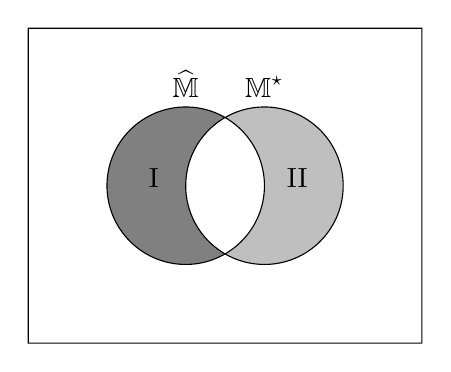
\begin{tikzpicture}[fill]
% left hand
\scope
\clip (-2,-2) rectangle (2,2)
      (1,0) circle (1);
\fill[gray] (0,0) circle (1);
\endscope
% right hand
\scope
\clip (-2,-2) rectangle (2,2)
      (0,0) circle (1);
\fill[lightgray] (1,0) circle (1);
\endscope
% outline
\draw (0,0) circle (1) (0,1)  node [text=black,above] {$\displaystyle \hat{{\bbM}}$}
      (1,0) circle (1) (1,1)  node [text=black,above] {$\displaystyle {\bbM}^{\star}$}
      (-2,-2) rectangle (3,2);
      
% Text Node
\draw (1.25,0.25) node [anchor=north west][inner sep=0.75pt]   [align=left] {II};
% Text Node
\draw (-0.5,0.25) node [anchor=north west][inner sep=0.75pt]   [align=left] {I};
      
      
      
\end{tikzpicture}
%\label{fig:error-visual}
\caption{Visualization of the two types of errors}

\end{figure}

For convenience, we introduce some additional notation. Let ${\bbM}^\star_d$ be the true model on the $d$-way interactions. Then 
\begin{align*}
    {\bbM^\star} = {\bbM}^\star_1\cup\cdots\cup{\bbM}^\star_D.
\end{align*}
Analogously we can define the sample version of these concepts. That is, let 
\begin{align*}
    \hat{\bbM} = \hat{\bbM}_1\cup\cdots\cup\hat{\bbM}_D.
\end{align*}

One important part in understanding Algorithm \ref{alg:forward-ms} is that it introduces two operators to advance the selected working models to the next layer. Concretely speaking, Step \ref{alg:step-prune} - Step \ref{alg:strong-prune} introduces a deterministic operator $\texttt{P}(\cdot)$ on a given model $\bbM$, while Step \ref{alg:BC-1} - Step \ref{alg:BC-3} introduces a stochastic (or data dependent) operator $ \hat{\texttt{S}}(\cdot) =  \hat{\texttt{S}}(\cdot; \{Y_i,X_i\}_{i=1}^N)$ on any given model $\bbM$.  We can track the models in the following diagram:
\begin{align}%\label{eqn:track-model}
    \hat{\bbM}_{1}\xrightarrow{\texttt{P}}\cdots\xrightarrow{ \hat{\texttt{S}}}\hat{\bbM}_{d-1}\xrightarrow{\texttt{P}}\hat{\bbM}_{d,+}\xrightarrow{ \hat{\texttt{S}}}\hat{\bbM}_{d}\to \cdots \xrightarrow{ \hat{\texttt{S}}} \hat{\bbM}_{D}.
\end{align}

Intuitively speaking, in order to achieve satisfactory  screening results, some regularization conditions need to be imposed to characterize a ``good" layer-wise selection method. A key question is that: if we are able to select the $(d-1)$-th layer correctly, can the selection procedure forwards the good results to the $d$-th layer?  In light of this, we use ${\bbM}^\star_{d,+}$ to denote the pruned set of effects on the $d$-th layer based on the true model $\bbM_{d-1}^\star$ on the previous layer; that is,
\begin{align*}
    {\bbM}^\star_{d,+} = \texttt{P}({\bbM}^\star_{d-1}).
\end{align*}
These discussions motivate the following assumption on the layer-wise selection procedure $ \hat{\texttt{S}}(\cdot)$:
\begin{assumption}[Validity and consistency of the selection operator]%\label{assume:valid-consistent}
We denote 
\begin{align*}
    \tilde{\bbM}_{d} = \text{\em \texttt{S}}_N(\bbM^{\star}_{d,+};\{Y_i,X_i\}^N_{i=1}),
\end{align*}
where $\bbM^{\star}_{d,+} = \text{\em \texttt{P}}(\bbM^{\star}_{d-1})$ is defined as above. Let $\{\alpha_d\}_{d=1}^D$ be a sequence of significance levels in $(0,1)$. We assume that the following \emph{validity} and \emph{consistency} property hold for $\text{\em \texttt{S}}_N(\cdot)$: for $d = 1,\cdots, D$, we have
\begin{align}
    \text{Validity:}&~\lim\sup_{N\to\infty}\bbP\lt\{\tilde{\bbM}_{d}\cap\bbM^{\star c}_d\neq \varnothing\rt\}\le \alpha_d,  %\label{eqn:validity}
    \\
    \text{Consistency:}&~\lim\sup_{N\to\infty}\bbP\lt\{\tilde{\bbM}_{d}^c\cap\bbM^{\star}_d\neq \varnothing\rt\} = 0.  %\label{eqn:consistency}
\end{align}
\end{assumption}

This assumption can be proved for many  screening procedures. In Corollary \ref{cor:marginal-t} we will show it holds for the layer-wise Bonferroni corrected marginal testing procedure in Algorithm \ref{alg:forward-ms}. Moreover, in the high dimensional super population study, data splitting and adaptation of $\ell_1$ regularization can also fulfill such a requirement \citep{wasserman2009high}.


\begin{theorem}[ screening consistency]%\label{thm:ms-consistency}

Assume $\bbM^\star\neq\varnothing$. Assume Condition \ref{cond:heredity} holds.  
Let $D$ be the largest positive integer such that there is at least one nonzero $D$-order interaction effects. Then Algorithm 1 with default weights and maximal interaction levels $D$ has the following properties:

\begin{enumerate}
    \item {\em Type I error control.} Algorithm 1 controls the Type I error rate, in the sense that 
    \begin{align}
        \underset{N_k\to\infty,~\forall k\in[K]}{\lim\sup}\bbP\left(\hat{\bbM}\cap{\bbM^\star}^c\neq\varnothing\right)\le \alpha.
    \end{align}
    \item {\em  screening consistency.} Further assume $\alpha=\alpha_N\to0$. Algorithm 1 consistently selects all the non-null terms with probability tending to 1: 
    \begin{align}
        \underset{N_k\to\infty,~\forall k\in[K]}{\lim\sup}\bbP\left(\hat{\bbM}=\bbM^\star\right)=1.
    \end{align}
\end{enumerate}
\end{theorem}


\begin{corollary}[Bonferroni corrected marginal test]
Let $\tilde{\bbM}_{d} = \cS_N(\bbM^{\star}_{d,+})$ where $\bbM^{\star}_{d,+} = \cP(\bbM^{\star}_{d-1})$. Assume the following scaling of parameters:
\begin{itemize}
    \item $|\tau_\cK| =  \Theta(N_0^\delta)$ for some $\delta > -1/2$ and all $\cK\in\bbM_d^\star$.
    \item ${\alpha_d} =  \Theta(N_0^{-\delta'})$ for some $\delta'\ge 0$.
\end{itemize} 
Also assume the conditions in Lemma \ref{lem:asp-results} hold. Then we have
the following results for the  screening procedure based on Bonferroni corrected marginal t-test:
\begin{enumerate}
    \item (Validity) $\lim\sup_{N\to\infty}\bbP\lt\{\tilde{\bbM}_{d}\cap\bbM^{\star c}_d\neq \varnothing\rt\}\le \alpha_d$ for all $d=1,\cdots,D$.
    \item (Consistency) $\lim\sup_{N\to\infty}\bbP\lt\{\tilde{\bbM}_{d}^c\cap\bbM^{\star}_d\neq \varnothing\rt\} = 0$ for all $d=1,\cdots,D$.
    \item (Type I error control) Overall the procedure achieves family-wise error rate control:
    \begin{align*}
    \underset{N\to\infty}{\lim\sup}~\bbP\left(\hat{\bbM}\cap{\bbM^\star}^c\neq \varnothing\right)
    \le 
    \frac{\alpha_1}{K}\cdot|\bbM_1^\star| + \sum_{d=2}^D \frac{\alpha_d}{|\bbM^\star_{d,+}|}\cdot|\bbM^\star_d| \le \alpha.
    \end{align*}
    \item (Perfect selection) When $\delta'<0$, $\alpha_d\to0$, 
    \begin{align*}
    \underset{N\to\infty}{\lim}~\bbP\left(\hat{\bbM} = {\bbM^\star}  \right)
     = 1.
    \end{align*}
\end{enumerate}

\end{corollary}

\textbf{Benefits of heredity.} It is well-known that Bonferroni correction controls Type I error rate at the cost of inflated type II error rates. The heredity structure can alleviate this inflation by reducing the number of tests we need to work on within each level. Mathematically, from the proof, by our calculation, in the $k$-th step the Type II error of the Bonferroni correction is upper bounded by 
\begin{align}\label{eqn:type-II}
        &\underset{N\to\infty}{\lim\sup}~\bbP\lt\{\tilde{\bbM}^c_{d}\cap\bbM^{\star }_d\neq \varnothing\rt\} \notag\\
        & \le \underset{N\to\infty}{\lim\sup}~\sum_{\cK\in\bbM_d^\star} \Phi\lt\{r_\cK^{-1}\lt(Z_d^\star - \frac{\tau_\cK}{\sigma_\cK}\rt)\rt\} - \Phi\lt\{r_\cK^{-1}\lt(-Z_d^\star - \frac{\tau_\cK}{\sigma_\cK}\rt)\rt\},
\end{align}
where
\begin{align*}
    Z_d^\star = \sqrt{2\ln\frac{2|\bbM_{d,+}^\star|}{\alpha_d}} + o(1), \text{ as } \alpha_d \to 0.
\end{align*}

On the other hand, one can easily formulate a lower bound:
\begin{align}\label{eqn:type-II-lb}
        &\underset{N\to\infty}{\lim\sup}~\bbP\lt\{\tilde{\bbM}^c_{d}\cap\bbM^{\star }_d\neq \varnothing\rt\} \notag\\
        & \ge \underset{N\to\infty}{\lim\sup}~\max_{\cK\in\bbM_d^\star} \Phi\lt\{r_{\cK}^{-1}\lt(Z_d^\star - \frac{\tau_\cK}{\sigma_\cK}\rt)\rt\} - \Phi\lt\{r_{\cK}^{-1}\lt(-Z_d^\star - \frac{\tau_\cK}{\sigma_\cK}\rt)\rt\}.
\end{align}

Since we are considering fixed dimension, the bounds \eqref{eqn:type-II} and \eqref{eqn:type-II-lb} are almost tight up to a factor $|\bbM^\star_{d}|$. Hence it's important to characterize the rate of the following quantity for any $\cK\in\bbM_d^\star$:
\begin{align*}
    \Phi\lt\{r_{\cK}^{-1}\lt(Z_d^\star - \frac{\tau_\cK}{\sigma_\cK}\rt)\rt\} - \Phi\lt\{r_{\cK}^{-1}\lt(-Z_d^\star - \frac{\tau_\cK}{\sigma_\cK}\rt)\rt\}.
\end{align*}

When there is no heredity structure, a full Bonferroni correction would give
\begin{align*}
    \tilde{Z}_d^\star = \sqrt{2\ln\frac{2{K \choose d}}{\alpha_d}} + o(1), \text{ as } \alpha_d \to 0.
\end{align*}
WLOG we assume $\tau_\cK > 0$. Consider each summand in \eqref{eqn:type-II}; the leading term would be the first component:
$\Phi\lt\{r_\cK^{-1}\lt(Z_d^\star - \frac{\tau_\cK}{\sigma_\cK}\rt)\rt\}$. Asymptotically, when $\alpha_d\to 0$,  we have
\begin{align*}
    \lim_{N\to\infty}\frac{\Phi\lt\{r_{\cK}^{-1}\lt(Z_d^\star - \frac{\tau_\cK}{\sigma_\cK}\rt)\rt\}}{\Phi\lt\{r_\cK^{-1}\lt(\tilde{Z}_d^\star - \frac{\tau_\cK}{\sigma_\cK}\rt)\rt\}}
    = & \lim_{N\to\infty}\frac{ \frac{1}{\sqrt{2\pi}} \exp\lt\{ -\frac{(\tau_\cK/\sigma_\cK-Z_d^\star)^2}{2r^2_\cK} \rt\} }{ \frac{1}{\sqrt{2\pi}} \exp\lt\{ -\frac{(\tau_\cK/\sigma_\cK-\tilde{Z}_d^\star)^2}{2r^2_\cK} \rt\}} \see{L'Hopital's rule}\\
    = & \lim_{N\to\infty}\exp\lt\{\frac{\tilde{Z}_d^{\star 2} - Z_d^{\star 2}}{2r_\cK^2}\rt\}\cdot \exp\lt\{\frac{\tau_\cK(Z_d^\star - \tilde{Z}_k^\star)}{\sigma_\cK r_\cK^2}\rt\}\\
    = & \lim_{N\to\infty} \lt\{\frac{|\bbM^\star_{d,+}|}{{K \choose d}}\rt\}^{-\frac{1}{2r_\cK^2}} \cdot \exp\lt\{-\frac{\tau_\cK(\tilde{Z}_d^\star - {Z}_d^\star)}{\sigma_\cK r_\cK^2}\rt\}.
\end{align*}

We know that
\begin{align*}
    \tilde{Z}_d^\star - {Z}_d^\star = \frac{\tilde{Z}_d^{\star2} -  {Z}_d^{\star2}}{Z_d^\star + \tilde{Z}_d^\star} = \frac{2\ln\{{K \choose d}/|\bbM^\star_{d,+}|\}}{2\sqrt{\ln{\frac{1}{\alpha_d}}}}\{1+o(1)\}.
\end{align*}

Hence 
\begin{align*}
    \lim_{N\to\infty}\frac{\Phi\lt\{r_{\cK}^{-1}\lt(Z_d^\star - \frac{\tau_\cK}{\sigma_\cK}\rt)\rt\}}{\Phi\lt\{r_{\cK}^{-1}\lt(\tilde{Z}_d^\star - \frac{\tau_\cK}{\sigma_\cK}\rt)\rt\}}
    = & \lim_{N\to\infty} \lt\{\frac{|\bbM^\star_{d,+}|}{{K \choose d}}\rt\}^{\frac{\tau_\cK\{1+o(1)\}}{\sigma_\cK r_\cK^2\sqrt{\ln(1/\alpha_k)}}-\frac{1}{2r_\cK^2}}.
\end{align*}

Now by our assumption, $\alpha_d =  \Theta(N^{-\delta'})$ for some $\delta' \ge 0$, $\tau_\cK =  \Theta(N^\delta)$ for some $\delta>-1/2$, 
\begin{align*}
    \frac{\tau_\cK\{1+o(1)\}}{\sigma_\cK r_\cK^2\sqrt{\ln(1/\alpha_d)}}-\frac{1}{2r_\cK^2} =  \Theta\lt(\frac{N^{\delta + 1/2}}{\max\{\delta'\ln N,1\}}\rt).
\end{align*}

To sum up, within the $d$-th level, the ratio of the Type II error rate with/without heredity assumptions has the order of
\begin{align}\label{eqn:typeII-ratio}
    O\lt\{\lt({|\bbM^\star_{d,+}|}/{K \choose d}\rt)^{\frac{CN^{\delta + 1/2}}{\max\{\delta'\ln N,1\}}}\rt\}.
\end{align}

This shows that the heredity assumption can significantly reduce the type II error and improve the power of the selection procedure if the true effects have sparse structure (that is, $|\bbM_d^\star|$ is much smaller than the total number of $d$-way effects ${K \choose d}$).  


\subsection{Factor level combination selection from a non-asymptotic view}

We generalize the definition of the tiers \eqref{def:tiers} to embrace a non-asymptotic study of the factor level combination selection results.  Suppose there exists $H$ scalars $\overline{Y}_{(1)} > \cdots > \overline{Y}_{(H)}$, with which the set of $\Gamma_{K_0}$ can be partitioned into $H$ tiers:
\begin{align}\label{eqn:near-tie}
    \Gamma_{K_0;h} = \lt\{\overline{Y}(\bz)\in\Gamma_{K_0}\mid|\overline{Y}(\bz) - \overline{Y}_{(h)}| = o(N_0^{-\delta_3})\rt\}, h = 1,\cdots,H.
\end{align}
Now we define
\begin{align*}
    d_h = \max_{\bz\in\cT_{K_0;h} } |\overline{Y}(\bz) - \overline{Y}_{(h)}|, ~d^\star_h = \min_{\bz\notin\cT_{K_0;h}} |\overline{Y}(\bz) - \overline{Y}_{(h)}|.
\end{align*}
which we refer to as within-group distance and between-group distance respectively. 



\commenting{
\note{red}{(Alternatively we can assume the following two conditions. But I did not show the rates associated with them yet)} With more conditions, we can perform Edgeworth expansion\citep{shao2012jackknife} to get better rates:
\begin{condition}\label{cond:edgeworth}
There exists universal constants $A,B,L>0$, such that for all $k\in[K]$ 
\begin{align*}
    \sup_{t\in \bbR} \lt|\bbP\lt\{\frac{\sqrt{N}(\hat{\gamma}_k - \gamma_k)}{s_k} < t\rt\} -  \Phi(t) - (At^2+B)\phi(t)N^{-\frac{1}{2}}\rt| \le LN^{-1}.
\end{align*}
\end{condition}
}




\begin{theorem}[Convergence of the selected tie sets]%\label{thm:wt-converge}
Assume the following regularization condition on the variance of $\hat{Y}_{\operatorname{AVG}}$, $V$:
\begin{align*}
    \lambda_{\min}(N_0 V) \ge \underline{\lambda}.
\end{align*}
Also assume Assumption \ref{assume:design}, \ref{assume:sparse} and \ref{cond:heredity} hold. Assume the following scaling of parameters: $d_h^\star= \Theta(N_0^{\delta_1}), \eta_N = \Theta(N_0^{\delta_2}), d_h = \Theta(N_0^{\delta_3})$ with $-1/2 < \delta_1 < \delta_2 < \delta_3$.
Let $\underline{\epsilon}<\overline{\epsilon}$ be two positive real numbers. If we select the factor level combinations using Algorithm \ref{alg:comb-selection}, taking $b_L =  b_R = 2\underline{\epsilon}\eta_N$, when $N_0$ is large enough, i.e.,  $N_0>n_0(\delta_1,\delta_2,\delta_3,\bar{\epsilon}, \underline{\epsilon},\beta)$, it holds that
\begin{align*}
   &\bbP\lt\{\forall~h \in [H_0]: \hat{\cT}_{K_0;h} = {\cT}_{K_0;h} \rt\} \\
   \ge & 1 - \bbP\{\hat{\bbM}\neq \bbM^\star\} - 32\lt(\sum_{h=1}^{H_0}|\cT_{K_0;h}|\rt) |\Gamma_{K_0}| \frac{C \max_{i\in[N],\bz\in\cT}|\breve{Y}_i(\bz)| }{\sqrt{\underline{\lambda}}}\cdot \sqrt{\frac{|\bbM^\star|}{N_0 Q}}.
\end{align*}


\end{theorem}

\commenting{
\begin{remark}
To show the results, we assumed a delicate characterization of the distributional convergence rates in \eqref{eqn:berry-esseen}. In many cases, this corresponds to a Berry-Esseen type inequality; for example, \cite{shao2012jackknife, bentkus1996bberry, jing2000berry} proves bounds for i.i.d. data, and \cite{bolthausen1984estimate} for bounds of combinatorial type.
\end{remark}
}





\subsection{Inference of the ordered values}

In the previous sections, we have shown that, under certain conditions, we can select the true model $\bbM^\star$ and $\cT_{K_0;h}$ with high probability. Hence we could expect that Step \ref{alg:point-est} of Algorithm \ref{alg:forward-ms} would generate a sequence of point estimates 
\begin{align*}
    \frac{1}{|\hat{\cT}_{K_0;h}|} \sum_{\bz\in \hat{\cT}_{K_0;h}} \hY_{\operatorname{RP}}(\bz)
\end{align*}
that has similar asymptotic behavior as
\begin{align*}
    \frac{1}{|{\cT}_{K_0;h}|} \sum_{\bz\in {\cT}_{K_0;h}} \hY_{\operatorname{RP}}^\star(\bz)
\end{align*}
This can be rigorously summarized in the following theorem:

\begin{theorem}[Asymptotic results on the estimated effects]\label{thm:infer-order}
Let $Q$ be fixed. Assume the conditions in Lemma \ref{lem:asp-results}, Theorem \ref{thm:ms-consistency} and Theorem \ref{thm:wt-converge}. Then the point estimates are asymptotically jointly normal:
\begin{align*}
        \sqrt{N_0}\lt\{
        \begin{pmatrix}
        \hY_{(1)}\\
        \vdots \\
        \hY_{(H_0)}
        \end{pmatrix}
        - 
        \begin{pmatrix}
        \overline{Y}_{(1)}\\
        \vdots \\
        \overline{Y}_{(H_0)}
        \end{pmatrix} 
        \rt\} \to N(0, W^\top V_{\lim} W),
\end{align*}
where $W\in\bbR^{H_0 \times Q}$ has columns
\begin{align*}
    W_{\cdot h} = \sum_{\bz\in {\cT}_{K_0;h}}\frac{w_{\bz}}{|{\cT}_{K_0;h}|} = (Q|{\cT}_{K_0;h}|)^{-1}\sum_{\bz\in {\cT}_{K_0;h}}G_{\bbM^\star} G_{\bz, \bbM^\star}^\top .
\end{align*}
Moreover, $W^\top \hat{V}_R W$ is a robust variance estimator which satisfies
\begin{align*}
    {N_0} \{W^\top \hat{V}_R W - W^\top {V}_R W\} \xrightarrow{p} 0, ~ N_0 V_{R} \to V_{R,\lim}, ~ W^\top V_{R,\lim} W \succeq W^\top V_{\lim} W.
\end{align*}

\end{theorem}


\textbf{Benefits of reparametrization under sparsity.} Consider one simple scenario: only looking at the first tier ($H_0 = 1$) which only contains a single element $\bz_1$ ($|\cT_{K_0;h}| = 1$). Asymptotically speaking, we have
\begin{align*}
    \sqrt{N_0} \lt\{\hY_{\operatorname{AVG}}(\bz_1) - \overline{Y}(\bz_1)\rt\} &\xrightarrow{d} N(0, V_{\lim}(\bz_1,\bz_1));\\
    \sqrt{N_0} \lt\{\hY_{\operatorname{RP}}(\bz_1) - \overline{Y}(\bz_1)\rt\} &\xrightarrow{d} N(0, w_{\bz_1}^\top V_{\lim}w_{\bz_1}).
\end{align*}
When constructing confidence intervals, we would use robust variance estimation $\hat{V}_R(\bz_1,\bz_1)$ and $w_{\bz_1}^\top \hat{V}_R w_{\bz_1}$, which (after multiplied by $N_0$) have limits: 
\begin{align*}
    V_{R,\lim}(\bz_1,\bz_1) &= \frac{S_{\lim}(\bz_1,\bz_1)}{c_{\lim}(\bz_1)}, \\
    w_{\bz_1}^\top V_{R,\lim}w_{\bz_1} & = Q^{-2} G_{\bz_1, \bbM^\star}G_{\bbM^\star}^\top  V_{R,\lim}  G_{\bbM^\star} G_{\bz_1, \bbM^\star}^\top\\
    & \le \|w_{\bz_1}\|_\infty^2 \sum_{\bz\in\cT} V_{R,\lim}(\bz,\bz)\\
    & = \frac{|\bbM^\star|}{Q} \lt\{Q^{-1} \sum_{\bz\in\cT} \frac{S_{\lim}(\bz,\bz)}{c_{\lim}(\bz)}\rt\}.
\end{align*}
If $Q$ is not that large, then one can simply run saturated regression and estimate all the factorial effects. However, when $Q$ (or equivalently $K$) is large, clearly the confidence intervals based on reparametrization has more advantage when the model is actually sparse. 

\commenting{
\section{Bonferroni corrected  screening on finite population }

Before diving into next part,  we establish a concrete result for a selection procedure based on Bonferroni corrected marginal t-test in the following corollaries. We show its validity and consistency property and apply Theorem \ref{thm:ms-consistency} to show it achieves a more delicate Type I error rate control as well as exact  screening. Our discussion is divided into the following two scenarios: a fixed dimension setup and an increasing dimension setup.

\subsection{Increasing $K$ with sufficient units in each arm.}

We focus on the increasing $K$ setting with sufficient units in each arm.
\begin{itemize}
    \item $N(\bz) = c(\bz)N_0$, where $0 < \underline{c} \le c(\bz) \le \overline{c}$ for all $\bz\in \cT$.
    \item $K \le \gamma \log_2(N_0)$.
\end{itemize}
That is, 
    \begin{align*}
        \lim_{N\to\infty} \frac{N_z}{N} = e_z\in(0,1),~\forall ~ z\in\cT.
    \end{align*}
    Under this scenario, the marginal t-test is given by
    \begin{align*}
        \ind{\lt|\frac{\sqrt{N}\htau_{\cK}}{\hat{s}_\cK}\rt|\ge\Phi^{-1}\lt(1-\frac{\alpha_k}{2|\bbM^{\star c}_{k,+}|} \rt)},
    \end{align*}
    where we have
    \begin{align*}
        \htau_{\cK} = \frac{1}{2^{K}}g^\top_\cK \hat{Y}_{\operatorname{AVG}}, ~\hat{s}^2_\cK = \frac{1}{2^{2K}}g^\top_\cK \diag{N(\bz)^{-1}\hat{S}(\bz)} g_\cK.
    \end{align*}
    
    We prove the following asymptotic results for these quantities:
    \begin{proposition}
    
    \end{proposition}
    
    
    
    According to \cite{zhao2021regression}, $\hat{s}^2_\cK$ is a robust  estimation for the true variance of $\htau_\cK$; that is,
    \begin{align*}
        &N\hat{s}_\cK^2 - N\bbE\{\hat{s}_\cK^2\}\xrightarrow{p} 0,
        ~\text{where } N\bbE\{\hat{s}_\cK^2\} = \frac{N}{2^{2K}} g^\top_\cK \diag{N_z^{-1}{S}(z,z)} g_\cK \ge N\operatorname{Var}(\htau_{\cK}).
    \end{align*}
    Define 
    \begin{align*}
        \frac{\operatorname{Var}(\htau_\cK)}{\bbE(\hat{s}^2_\cK)} = \sigma_\cK^2 \le 1,
    \end{align*}
    then according to \cite{li2017general}, under certain conditions,  we have 
    \begin{align*}
        \frac{\htau_{\cK}}{\hat{s}_\cK} - \frac{\tau_\cK}{s_\cK} \xrightarrow{d} N\lt(0,\frac{\operatorname{Var}(\htau_\cK)}{\bbE(\hat{s}^2_\cK)}\rt) : = N(0,\sigma_\cK^2).
    \end{align*}


\begin{corollary}[Fixed $K$ and sufficient units in each arm]\label{cor:marginal-t}
Let $\tilde{\bbM}_{k} = \cS_N(\bbM^{\star}_{k,+})$ where $\bbM^{\star}_{k,+} = \cP(\bbM^{\star}_{k-1})$. Assume the following scaling of parameters:
\begin{itemize}
    \item $\lim_{N\to\infty} \frac{N_z}{N} = e_z\in(0,1),~\forall ~ z\in\cT.$
    \item $|\tau_\cK| =  \Theta(N^\delta)$ for some $\delta > -1/2$ and all $\cK\in\bbM_k^\star$.
    \item ${\alpha_k} =  \Theta(N^{-\delta'})$ for some $\delta'\ge 0$.
\end{itemize} 
Assume the following conditions on the potential outcomes based on Theorem 5 of \cite{li2017general}:
\begin{itemize}
    \item $S(z,z')$ has limiting values, for all $z,z'\in\cT$. 
    \item $\max_{z\in\cT,i\in[N]} |Y_i(z) - \overline{Y}(z)|^2 /N \to 0$.
\end{itemize}
The following results hold for the  screening procedure based on Bonferroni corrected marginal t-test:
\begin{enumerate}
    \item (Asymptotic convergence) The estimates $\htau_\cK$ converges in distribution:
    \begin{align*}
        \frac{\htau_{\cK} - \tau_\cK}{\sqrt{\operatorname{Var}(\htau_\cK)}} \xrightarrow{d} N\lt(0,1\rt).
    \end{align*}
    The robust variance estimates converge in probability:
    \begin{align*}
        N\hat{s}^2_\cK - N\bbE\{\hat{s}_\cK^2\} \xrightarrow{p} 0.
    \end{align*}
    
    \item (Validity) $\lim\sup_{N\to\infty}\bbP\lt\{\tilde{\bbM}_{k}\cap\bbM^{\star c}_k\neq \varnothing\rt\}\le \alpha_k$ for all $k=1,\cdots,D$.
    \item (Consistency) $\lim\sup_{N\to\infty}\bbP\lt\{\tilde{\bbM}_{k}^c\cap\bbM^{\star}_k\neq \varnothing\rt\} = 0$ for all $k=1,\cdots,D$.
    \item (Type I error control) Overall the procedure achieves family-wise error rate control:
    \begin{align*}
    \underset{N\to\infty}{\lim\sup}~\bbP\left(\hat{\bbM}\cap{\bbM^\star}^c\neq \varnothing\right)
    \le 
    \frac{\alpha_1}{K}\cdot|\bbM_1^\star| + \sum_{k=2}^D \frac{\alpha_k}{|\bbM^\star_{k,+}|}\cdot|\bbM^\star_k| \le \alpha.
    \end{align*}
    \item (Perfect selection) When $\delta'<0$, $\alpha_k\to0$, 
    \begin{align*}
    \underset{N\to\infty}{\lim}~\bbP\left(\hat{\bbM} = {\bbM^\star}  \right)
     = 1.
    \end{align*}
\end{enumerate}

\end{corollary}
}








\section{Simulation studies}\label{sec:simulation}
We consider a factorial experiment with $5$ binary factors $F_1, \cdots, F_5$. The potential outcomes are generated independently from some gaussian super populations with varying means and constant standard deviation of one.  That is to say, 
\begin{align*}
    Y_i({\bz}) \sim N(\mu({\bz}), 1),~ \bz = (z_1,\cdots, z_5).
\end{align*}
In our experiments, we create $\mu(\bz)$ so that all the interaction effects of order three or higher are all zero. 

\subsection{Factorial structure under weak heredity}
In this subsection, we consider a specification of effects given by Figure \ref{fig:weak-factorial}. The effect sizes are determined in the following way: to impose sparsity in the model, we put the main effects $\tau_4$ and $\tau_{5}$ to be zero. Under weak heredity, the interaction terms involving $F_4,F_5$ all have to be zero.  For the rest of the main effects, we pick them independently from a uniform distribution $U([-5,-1]\cup [1,5])$ to ensure a nonzero magnitude. For the rest of the interactions,  we also choose them independently from $U([-5,-1]\cup [1,5])$; but to allow for zero size we introduce a censoring probability of $0.3$. That is, there is a variable $B\sim \operatorname{Ber}(0.3)$ independent of a uniform $U\sim U([-5,-1]\cup [1,5])$ such that $\tau_{kl}\sim U \cdot B$. We generate the finite population matrix from gaussian distributions with standard deviation 1, then permute the units among the $2^5$ treatment combinations, each arm with $100$ replications.  The Monte Carlo simulation is repeated for 500 runs.  Table \ref{tab:weak-ms} reports the  screening results based on several methods and heredity principles, and Table \ref{tab:weak-tier} reports the tier selection results, the confidence interval (CI) coverage rates along with the length of CIs. 

For the  screening results, we see that both Bonferroni correction and LASSO can achieve a high probability of selection consistency. Taking the weak heredity structure and forward procedure into account, the performance would be slightly better than running a full selection over the whole model. But since the number of factors $K$ is not too large here, the results does not demonstrate a large advantage.

For the Tier selection results, we see that under forward selection, the probability of perfect tier selection rises significantly. Besides, we can achieve better coverage rates for the confidence intervals. More importantly, the length of the CIs are much shorter compared to the case where we utilize naive group-wise averages, which verifies our theoretical discussion that we can borrow information across groups to improve the efficiency of the methods.



\begin{figure}
\centering
\tikzset{every picture/.style={line width=0.75pt}} %set default line width to 0.75pt
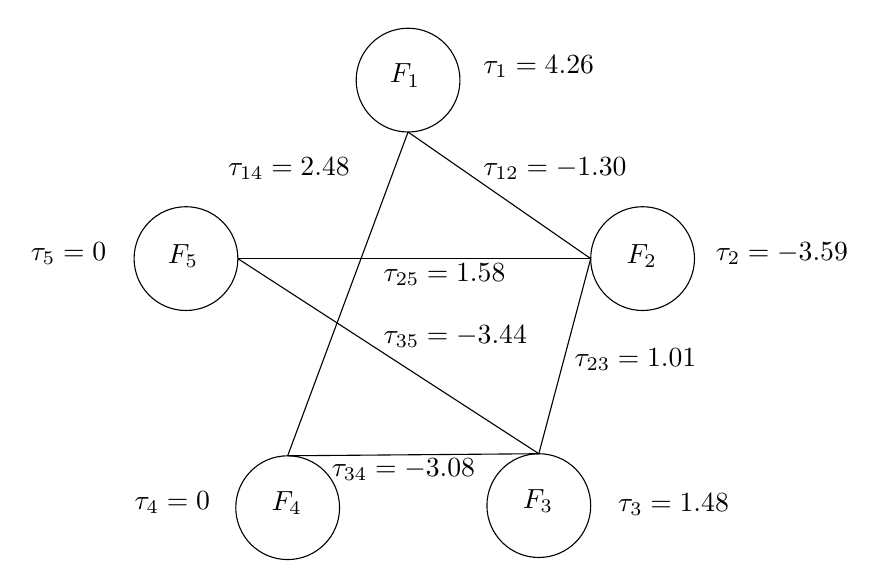
\begin{tikzpicture}[x=0.75pt,y=0.75pt,yscale=-1,xscale=1]
%uncomment if require: \path (0,300); %set diagram left start at 0, and has height of 300

%Shape: Circle [id:dp4313014510558797] 
\draw   (176,125) .. controls (176,111.19) and (187.19,100) .. (201,100) .. controls (214.81,100) and (226,111.19) .. (226,125) .. controls (226,138.81) and (214.81,150) .. (201,150) .. controls (187.19,150) and (176,138.81) .. (176,125) -- cycle ;
%Shape: Circle [id:dp5998957101320532] 
\draw   (225,245) .. controls (225,231.19) and (236.19,220) .. (250,220) .. controls (263.81,220) and (275,231.19) .. (275,245) .. controls (275,258.81) and (263.81,270) .. (250,270) .. controls (236.19,270) and (225,258.81) .. (225,245) -- cycle ;
%Shape: Circle [id:dp9946890814101954] 
\draw   (346,244) .. controls (346,230.19) and (357.19,219) .. (371,219) .. controls (384.81,219) and (396,230.19) .. (396,244) .. controls (396,257.81) and (384.81,269) .. (371,269) .. controls (357.19,269) and (346,257.81) .. (346,244) -- cycle ;
%Shape: Circle [id:dp8016116391819108] 
\draw   (283,39) .. controls (283,25.19) and (294.19,14) .. (308,14) .. controls (321.81,14) and (333,25.19) .. (333,39) .. controls (333,52.81) and (321.81,64) .. (308,64) .. controls (294.19,64) and (283,52.81) .. (283,39) -- cycle ;
%Shape: Circle [id:dp9137017243233785] 
\draw   (396,125) .. controls (396,111.19) and (407.19,100) .. (421,100) .. controls (434.81,100) and (446,111.19) .. (446,125) .. controls (446,138.81) and (434.81,150) .. (421,150) .. controls (407.19,150) and (396,138.81) .. (396,125) -- cycle ;
%Straight Lines [id:da2974493386223376] 
\draw    (308,64) -- (396,125) ;
%Straight Lines [id:da6535801803717902] 
\draw    (308,64) -- (250,220) ;
%Straight Lines [id:da7348008754063038] 
\draw    (226,125) -- (371,219) ;
%Straight Lines [id:da7061898459119043] 
\draw    (226,125) -- (396,125) ;
%Straight Lines [id:da8607213145000236] 
\draw    (396,125) -- (371,219) ;
%Straight Lines [id:da7049142157601076] 
\draw    (250,220) -- (371,219) ;

% Text Node
\draw (298,30) node [anchor=north west][inner sep=0.75pt]   [align=left] {$F_1$};
% Text Node
\draw (412,117) node [anchor=north west][inner sep=0.75pt]   [align=left] {$F_2$};
% Text Node
\draw (191,117) node [anchor=north west][inner sep=0.75pt]   [align=left] {$F_5$};
% Text Node
\draw (241,236) node [anchor=north west][inner sep=0.75pt]   [align=left] {$F_4$};
% Text Node
\draw (362,235) node [anchor=north west][inner sep=0.75pt]   [align=left] {$F_3$};
% Text Node
\draw (343,26) node [anchor=north west][inner sep=0.75pt]   [align=left] {$\tau_1 = 4.26$};
% Text Node
\draw (455,116) node [anchor=north west][inner sep=0.75pt]   [align=left] {$\tau_2 = -3.59$};
% Text Node
\draw (408,237) node [anchor=north west][inner sep=0.75pt]   [align=left] {$\tau_3 = 1.48$};
% Text Node
\draw (175,236) node [anchor=north west][inner sep=0.75pt]   [align=left] {$\tau_4 = 0$};
% Text Node
\draw (125,116) node [anchor=north west][inner sep=0.75pt]   [align=left] {$\tau_5 = 0$};
% Text Node
\draw (220,75) node [anchor=north west][inner sep=0.75pt]   [align=left] {$\tau_{14} = 2.48$};
% Text Node
\draw (295,156) node [anchor=north west][inner sep=0.75pt]   [align=left] {$\tau_{35} = -3.44$};
% Text Node
\draw (295,126) node [anchor=north west][inner sep=0.75pt]   [align=left] {$\tau_{25} = 1.58$};
% Text Node
\draw (270,220) node [anchor=north west][inner sep=0.75pt]   [align=left] {$\tau_{34} = -3.08$};
% Text Node
\draw (343,75) node [anchor=north west][inner sep=0.75pt]   [align=left] {$\tau_{12} = -1.30$};
% Text Node
\draw (387,167) node [anchor=north west][inner sep=0.75pt]   [align=left] {$\tau_{23} = 1.01$};
\end{tikzpicture}
\caption{Synthetic factorial effects specification under weak heredity. No edge between two nodes means the interaction is zero.}
\label{fig:weak-factorial}
\end{figure}




\begin{table}[ht]
\centering
\caption{ screening for factorial structure generated under weak heredity}
\label{tab:weak-ms}
\begin{tabular}{cccccc}
\toprule
Selection                   & Heredity        & Perfect  & Over  & Under  & None of above \\ \hline
\multirow{4}{*}{Bonferroni} & No heredity     & 0.974             & 0.026          & 0               & 0             \\ \cline{2-6} 
                            & Weak heredity   & 0.978             & 0.022          & 0               & 0             \\ \cline{2-6} 
                            & Strong heredity & 0                 & 0              & 0.978           & 0.022         \\ \cline{2-6} 
                            & Full WLS        & 0.972             & 0.026          & 0               & 0             \\ \hline
\multirow{4}{*}{LASSO}      & No heredity     & 0.974             & 0.020          & 0               & 0             \\ \cline{2-6} 
                            & Weak heredity   & 0.980             & 0              & 0               & 0             \\ \cline{2-6} 
                            & Strong heredity & 0                 & 0.028          & 1.000           & 0             \\ \cline{2-6} 
                            & Full WLS        & 0.962             & 0.038          & 0               & 0             \\ \bottomrule
\end{tabular}
\end{table}




% Please add the following required packages to your document preamble:
% \usepackage{multirow}
% Please add the following required packages to your document preamble:
% \usepackage{multirow}
\begin{table}[ht]
\centering
\caption{Tier selection and inference for factorial structure generated under weak heredity}
\label{tab:weak-tier}
\begin{tabular}{ccccc}
\toprule
        Selection           &   Heredity. & Tier Selection & Coverage & CI length \\ \hline
\multirow{3}{*}{Bonferroni} & No heredity & 0.998          & 0.950    & 0.1828    \\ \cline{2-5} 
                            & Weak        & 0.998          & 0.950    & 0.1828    \\ \cline{2-5} 
                            & Strong      & 0.000          & 0.000    & 1.0470    \\ \hline
\multirow{3}{*}{LASSO}      & No heredity & 1.000          & 0.952    & 0.1830    \\ \cline{2-5} 
                            & Weak        & 1.000          & 0.000    & 0.1829    \\ \cline{2-5} 
                            & Strong      & 0.000          & 0.950    & 1.0500    \\ \hline
No selection                & No heredity & 0.960          & 0.936    & 0.2815    \\ \bottomrule
\end{tabular}
\end{table}





\subsection{Factorial structure under strong heredity}
In this subsection, we consider a specification of effects similar to the above setup but generated under strong heredity. The results are summarized in Table \ref{tab:strong-ms} and \ref{tab:strong-tier}. In this case we have a sparser model, and since the strong heredity structure holds for the parameters, proceeding with this prior knowledge can lead to a better  screening result. Moreover, as we highlight earlier, we would also have better coverage and shorter confidence intervals after taking the structure into account. 

% Please add the following required packages to your document preamble:
% \usepackage{multirow}
\begin{table}[th]
\centering
\caption{ screening for factorial structure generated under strong heredity}
\label{tab:strong-ms}
\begin{tabular}{cccccc}
\toprule
Selection                   & Heredity        & Perfect & Over  & Under & None of above \\ \hline
\multirow{4}{*}{Bonferroni} & No heredity     & 0.974   & 0.026 & 0     & 0             \\ \cline{2-6} 
                            & Weak heredity   & 0.974   & 0.026 & 0     & 0             \\ \cline{2-6} 
                            & Strong heredity & 0.986   & 0.014 & 0     & 0             \\ \cline{2-6} 
                            & Full WLS        & 0.970   & 0.032 & 0     & 0             \\ \hline
\multirow{4}{*}{LASSO}      & No heredity     & 0.968   & 0.034 & 0     & 0             \\ \cline{2-6} 
                            & Weak heredity   & 0.966   & 0.006 & 0     & 0             \\ \cline{2-6} 
                            & Strong heredity & 0.994   & 0.030 & 0     & 0             \\ \cline{2-6} 
                            & Full WLS        & 0.966   & 0.034 & 0     & 0             \\ \bottomrule
\end{tabular}
\end{table}



\begin{table}[ht]
\centering
\caption{Tier selection and inference for factorial structure generated under strong heredity}
\label{tab:strong-tier}
\begin{tabular}{ccccc}
\toprule
        Selection           & Heredity    & Tier Selection & Coverage & CI length \\ \hline
\multirow{3}{*}{Bonferroni} & No heredity & 1.000          & 0.950    & 0.2062    \\ \cline{2-5} 
                            & Weak        & 1.000          & 0.950    & 0.2062    \\ \cline{2-5} 
                            & Strong      & 1.000          & 0.950    & 0.2062    \\ \hline
\multirow{3}{*}{LASSO}      & No heredity & 1.000          & 0.950    & 0.2062    \\ \cline{2-5} 
                            & Weak        & 1.000          & 0.950    & 0.2062    \\ \cline{2-5} 
                            & Strong      & 1.000          & 0.950    & 0.2062    \\ \hline
No selection                & No heredity & 0.974          & 0.938    & 0.2763    \\ \bottomrule
\end{tabular}
\end{table}

\subsection{Many factors with limited number of replications in each arm}


\section{Case study}

\section{Technical proofs}

\subsection{Proof of Theorem \ref{thm:ms-consistency}}

\begin{proof}
\textbf{Induction proof of a basic fact.} According to the orthogonality of designs, the signs for all terms in the studied unsaturated population regressions are consistent with those of saturated regressions, which saves the effort of differentiating true models for partial and full regression. By induction we hope to prove the following fact under the given assumptions:


\begin{displayquote}
For all $D_0\le D$, we have 
\begin{align}%\label{eqn:zerofn-general}
\lt|\bbP\lt(\hat{\bbM}_d\subset\bbM^\star_d, d=1,\cdots,D_0\rt)-\bbP\lt(\hat{\bbM}_d=\bbM^\star_d, d=1,\cdots,D_0\rt)\rt|\to 0.
\end{align} 
\end{displayquote}

Clearly we know the following inclusion is always true: for any $D_0\in[D]$,
$$\lt\{\hat{\bbM}_d=\bbM^\star_d, d=1,\cdots,D_0\rt\}\subset\lt\{\hat{\bbM}_d\subset\bbM^\star_d, d=1,\cdots,D_0\rt\}.$$ 
Hence the statement \eqref{eqn:zerofn-general} is equivalent to: for all $D_0\le D$,
\begin{align}%\label{eqn:zerofn-general-1}
\bbP\lt(\forall d\in[D_0],\hat{\bbM}_d\subset\bbM^\star_d; \exists d\in[D_0], \hat{\bbM}_d\subsetneq\bbM^\star_d\rt)\to 0.
\end{align} 


\begin{enumerate}
    \item \textbf{Main effects.}
    First, since we assume the tests are consistent, meaning asymptotically no false negatives:
    \begin{align*}
        \bbP\left({\hat{\bbM}_1}^c \cap\bbM^\star_1\neq \varnothing\right)\to 0.
    \end{align*}
    Or equivalently, 
    \begin{align*} 
        \bbP\left(\bbM^\star_1\subset{\hat{\bbM}_1}\right)\to 1.
    \end{align*}
    
    That being said, 
    \begin{align}%\label{eqn:zerofn-general-2}
      \bbP\lt(\hat{\bbM}_1\subsetneq\bbM^\star_1\rt)\to 0.
    \end{align} 
    
    
    
    \item \textbf{Induction validity.}
    Generally speaking, the induction proceeds based on the following idea:
    

    
    The case for $D_0=1$ has been shown in the previous part. Now assume \eqref{eqn:zerofn-general} or \eqref{eqn:zerofn-general-1} is true for some $D_0\ge1$.  For $D_0+1$, 
    the following holds:
    \begin{align*} 
        0&\le \bbP\left(\left\{\hat{\bbM}_d\subset\bbM^\star_d, d\le D_0+1\right\}\right)-\bbP\left(\left\{\hat{\bbM}_d=\bbM^\star_d, d\le D_0; \hat{\bbM}_{D_0+1}\subset\bbM^\star_{D_0+1}\right\}\right) \\
        &= \bbP\left(\left\{\hat{\bbM}_d\subset\bbM^\star_d, d\le D_0+1\right\} - \left\{\hat{\bbM}_d=\bbM^\star_d, d\le D_0; \hat{\bbM}_{D_0+1}\subset\bbM^\star_{D_0+1}\right\}\right)\notag\\
        &\le \bbP\left(\forall d\in[D_0+1], \hat{\bbM}_{d}\subset\bbM^\star_{d}; \exists d\in[D_0], \hat{\bbM}_d\subsetneq\bbM^\star_d\right)\notag\\
        &\le \bbP\left(\forall d\in[D_0], \hat{\bbM}_{d}\subset\bbM^\star_{d};\exists d\in[D_0], \hat{\bbM}_d\subsetneq\bbM^\star_d\right)\to 0.\see{by \eqref{eqn:zerofn-general-1}}
    \end{align*}
    Hence
    \begin{align}%\label{eqn:zerofun-general-2}
        \lt|\bbP\left(\left\{\hat{\bbM}_d\subset\bbM^\star_d, d\le D_0+1\right\}\right) - 
        \bbP\left(\left\{\hat{\bbM}_d=\bbM^\star_d, d\le D_0; \hat{\bbM}_{D_0+1}\subset\bbM^\star_{D_0+1}\right\}\right)\rt| \to 0.
    \end{align}
    
    Now $\hat{\bbM}_{D_0+1}$ is generated based on $\hat{\bbM}_{D_0}$ and the set of estimates over the prescreened effect set  $\hat{\bbM}_{D_0+1,+}$. Due to the Step \ref{alg:step-prune} in Algorithm \ref{alg:forward-ms},  under Assumption \ref{cond:heredity}, on the event $\hat{\bbM}_d = \bbM_d^\star$ we have
    \begin{align*}
        \hat{\bbM}_{d+1} = \tilde{\bbM}_{d+1}.
    \end{align*}
    
    Hence we can compute
    \begin{align*}
        0\le& \bbP\left(\lt\{\hat{\bbM}_d=\bbM^\star_d, d\le D_0; \hat{\bbM}_{D_0+1}\subset\bbM^\star_{D_0+1}\rt\}\right) - \bbP\left(\hat{\bbM}_d=\bbM^\star_d, d\le D_0+1\right)\\
        = & \bbP\left(\hat{\bbM}_d=\bbM^\star_d, d\le D_0; \hat{\bbM}_{D_0+1}\subsetneq \bbM^{\star }_{D_0+1}\right) \\
        = & \bbP\left(\hat{\bbM}_d=\bbM^\star_d, d\le D_0; \tilde{\bbM}_{D_0+1}\subsetneq \bbM^{\star }_{D_0+1}\right) \\
        \le&  \bbP\left(\tilde{\bbM}^c_{D_0+1}\cap\bbM^{\star }_{D_0+1}\neq\varnothing\right)\to 0.
    \end{align*}
   The last convergence holds  because of the consistency of the test.
    
    The induction can be proceeded. 
    
    
    \textbf{Proof of the first result.} Now it follows
    \begingroup
    \allowdisplaybreaks
    \begin{align}
    &\underset{N\to\infty}{\lim\sup}~\bbP\left(\hat{\bbM}\cap{\bbM^\star}^c\neq\varnothing\right) \notag\\
    &= 
    \underset{N \to\infty}{\lim\sup}~\bbP\left(\hat{\bbM}_1\cap{\bbM_1^\star}^c\neq\varnothing\right) + \sum_{D_0=2}^{D} \bbP\left(\hat{\bbM}_d\cap{\bbM_d^\star}^c=\varnothing,d=1,\cdots,D_0-1; \hat{\bbM}_{D_0}\cap \bbM_{D_0}^{\star c}\neq\varnothing\right)\notag\\
    &=
    \underset{N \to\infty}{\lim\sup}~\bbP\left(\hat{\bbM}_1\cap{\bbM_1^\star}^c\neq\varnothing\right) + \sum_{D_0=2}^D \bbP\left( \hat{\bbM}_d=\bbM^\star_d,d=1,\cdots,D_0-1; \hat{\bbM}_{D_0}\cap{\bbM_{D_0}^{\star c}}\neq\varnothing\right) \notag\\
    &\see{using \eqref{eqn:zerofn-general} and the fact that $D$ is a fixed integer}\notag\\
    &\le \underset{N \to\infty}{\lim\sup}~\bbP\left(\hat{\bbM}_1\cap{\bbM_1^\star}^c\neq\varnothing\right) + \sum_{D_0=2}^D \bbP\left( \hat{\bbM}_d=\bbM^\star_d,d=1,\cdots,D_0-1; \tilde{\bbM}_{D_0}\cap\bbM_{D_0}^{\star c}\neq\varnothing\right)  \notag\\
    &\see{on the given event, $\hat{\bbM}_{D_0,+} = \cP(\hat{\bbM}_{D_0-1}) = \cP({\bbM}^\star_{D_0-1}) = {\bbM}^\star_{D_0,+}$ and $\hat{\bbM}_{D_0} = \cS_N(\hat{\bbM}_{D_0,+}) = \tilde{\bbM}_{D_0}$}\notag\\
    &\le \underset{N \to\infty}{\lim\sup}~\bbP\left(\hat{\bbM}_1\cap{\bbM_1^\star}^c\neq\varnothing\right) + \sum_{D_0=2}^D \bbP\left(  \tilde{\bbM}_{D_0}\cap{\bbM_{D_0}^\star}^c\neq\varnothing\right)
    \le \sum_{D_0=1}^D\alpha_{D_0} = \alpha. %\label{eqn:fwer-general}
\end{align}
\endgroup
Therefore the FWER gets controlled under $\alpha$.

\textbf{Proof of the second result.} Under $\alpha=\alpha_N\to0$, \eqref{eqn:fwer-general} implies $\hat{\bbM}\subset\bbM^\star$ with probability tending to one, or
\[
\hat{\bbM}_d\subset\bbM^\star_d,  \text{ for } d=1,\cdots, D.
\]
Now apply \eqref{eqn:zerofn-general}, we obtain
\[
\hat{\bbM}_d=\bbM^\star_d,  \text{ for } d=1,\cdots, D,
\]
with probability tending to one, which concludes the proof.

\end{enumerate}

\end{proof}



\subsection{Proof of Corollary \ref{cor:marginal-t}}
\begin{proof}
\begin{enumerate}
    \item First we show validity. 
    \begin{align*}
        \underset{N\to\infty}{\lim\sup}~\bbP\lt\{\tilde{\bbM}_{d}\cap\bbM^{\star c}_d\neq \varnothing\rt\} 
        &= \underset{N\to\infty}{\lim\sup}~\bbP\lt\{\exists \cK\in\bbM^{\star }_{d,+}\backslash\bbM^{\star }_{d}, \lt|\frac{\htau_{\cK}}{\hat{\sigma}_\cK}\rt|\ge\Phi^{-1}\lt(1-\frac{\alpha_d}{2|\bbM^{\star }_{d,+}|} \rt)\rt\}\\
        &\le\underset{N\to\infty}{\lim\sup}~ \sum_{\cK\in\bbM^{\star }_{d,+}\backslash\bbM^{\star }_{d}} \bbP\lt\{\lt|\frac{\htau_{\cK}}{\hat{\sigma}_\cK}\rt|\ge\Phi^{-1}\lt(1-\frac{\alpha_d}{2|\bbM^{\star }_{d,+}|} \rt)\rt\}\\
        &\le \sum_{\cK\in\bbM^{\star }_{d,+}\backslash\bbM^{\star }_{d}} ~\frac{\alpha_d}{|\bbM^{\star }_{d,+}|} \le \alpha_d.
    \end{align*}
    \item Secondly, we show consistency.
    \begin{align*}
        \underset{N\to\infty}{\lim\sup}~\bbP\lt\{\tilde{\bbM}^c_{d}\cap\bbM^{\star }_d\neq \varnothing\rt\} 
        &= \underset{N\to\infty}{\lim\sup}~\bbP\lt\{\exists \cK\in \bbM^{\star }_{d}, \lt|\frac{\htau_{\cK}}{\hat{\sigma}_\cK}\rt|\le\Phi^{-1}\lt(1-\frac{\alpha_d}{2|\bbM^{\star }_{d,+}|} \rt)\rt\}\\
        &\le\underset{N\to\infty}{\lim\sup}~ \sum_{\cK\in\bbM^{\star }_{d}} \bbP\lt\{\lt|\frac{\htau_{\cK}}{\hat{\sigma}_\cK}\rt|\le\Phi^{-1}\lt(1-\frac{\alpha_d}{2|\bbM^{\star }_{d,+}|} \rt)\rt\}.
    \end{align*}
    Asymptotically we have
    \begin{align*}
        \frac{\htau_{\cK}}{\hat{\sigma}_\cK} - \frac{\tau_\cK}{\sigma_\cK} \xrightarrow{d} N\lt(0,\frac{\operatorname{Var}(\htau_\cK)}{\bbE(\hat{\sigma}^2_\cK)}\rt) : = N(0,r_\cK^2).
    \end{align*}
    For simplicity, let
    \begin{align*}
        Z_d^\star = \Phi^{-1}\lt(1-\frac{\alpha_d}{2|\bbM^{\star }_{d,+}|} \rt). 
    \end{align*}
    Hence
    \begin{align}
        &\underset{N\to\infty}{\lim\sup}~\bbP\lt\{\tilde{\bbM}^c_{d}\cap\bbM^{\star }_k\neq \varnothing\rt\} \notag\\
        &\le \underset{N\to\infty}{\lim\sup}~ \sum_{\cK\in\bbM^{\star }_{d}} \bbP\lt\{-\Phi^{-1}\lt(1-\frac{\alpha_d}{2|\bbM^{\star }_{d,+}|} \rt) - \frac{\tau_\cK}{\sigma_\cK}\le\frac{\htau_{\cK}}{\hat{\sigma}_\cK} - \frac{\tau_\cK}{\sigma_\cK}\le\Phi^{-1}\lt(1-\frac{\alpha_d}{2|\bbM^{\star }_{d,+}|} \rt) - \frac{\tau_\cK}{\sigma_\cK}\rt\}\notag\\
        & = \underset{N\to\infty}{\lim\sup}~\sum_{\cK\in\bbM_d^\star} \Phi\lt\{r_\cK^{-1}\lt(Z_d^\star - \frac{\tau_\cK}{\sigma_\cK}\rt)\rt\} - \Phi\lt\{r_\cK^{-1}\lt(-Z_d^\star - \frac{\tau_\cK}{\sigma_\cK}\rt)\rt\}.%\label{eqn:typeII-limit}
    \end{align}
    
     Note that when $\alpha_d\to 0, N\to\infty$, we have
    \begin{align*}
        Z_d^\star =  \Theta\lt(\sqrt{2\ln\frac{2|\bbM_{d,+}^\star|}{\alpha_d}}\rt) =  \Theta(\max\{\delta'\ln N,\ln(2|\bbM^\star_{d,+}|)\}),~ \lt|\frac{\tau_\cK}{\sigma_\cK}\rt| =  \Theta(N^{1/2+\delta}).
    \end{align*}
    Since $\delta>-1/2$ and $\delta'\ge 0$, we have $|\frac{\tau_\cK}{\sigma_\cK}| \to \infty$ and $Z_d^\star/(|\frac{\tau_\cK}{\sigma_\cK}|) \to 0$. Hence the above limit \eqref{eqn:typeII-limit} converges to zero. This concludes the proof.
    
    \item Based on the above two parts and Theorem \ref{thm:ms-consistency}, it suffices to conclude the Type I error rate control. A more delicate analysis in this particular setup can actually lead to sharper bound. Based on \eqref{eqn:fwer-general}, we directly compute
    \begin{align*}
    &\underset{N \to\infty}{\lim\sup}~\bbP\left(\hat{\bbM}\cap{\bbM^\star}^c\neq \varnothing\right) \\
    &\le\underset{N \to\infty}{\lim\sup}~\bbP\left(\hat{\bbM}_1\cap{\bbM_1^\star}^c\neq\varnothing\right) + \sum_{D_0=2}^D \bbP\left(  \tilde{\bbM}_{D_0}\cap{\bbM_{D_0}^\star}^c\neq\varnothing\right)\\
    &\le 
    \frac{\alpha_1}{K}\cdot|\bbM_1^\star| + \sum_{D_0=2}^D \frac{\alpha_{D_0}}{|\bbM^\star_{D_0,+}|}\cdot|\bbM^\star_{D_0}| \le \alpha. 
    \end{align*}
    
    \item The perfect selection result follows without difficult from Part 1,2 and Theorem \ref{thm:ms-consistency}.

\end{enumerate}
 
\end{proof}


\subsection{Proof of Theorem \ref{thm:wt-converge}}
\begin{proof}
The high level idea of the proof is that: we first prove the non-asymptotic bounds over the random event $\hat{\bbM} = \bbM^\star$, then proceed to make up for the cost of $\hat{\bbM} \neq \bbM^\star$. Over $\hat{\bbM} = \bbM^\star$, from Step \ref{alg:hatY-RP} of Algorithm \ref{alg:comb-selection} we have 
\begin{align*}
    \hat{Y}_{\operatorname{RP}} = \hat{Y}^\star_{\operatorname{RP}} = G_{\bbM^\star} \htau(\bbM^\star) = Q^{-1}G_{\bbM^\star}G_{\bbM^\star}^\top \hY_{\operatorname{AVG}}, ~\hGamma_{K_0} = \lt\{\hY^\star_{\operatorname{RP}}(z_1\cdots z_K)\mid \sum_{k=1}^K z_k \le K_0\rt\}.
\end{align*}
Under Assumption \ref{assume:sparse}, we have 
\begin{align*}
    \bbE\{\hat{Y}^\star_{\operatorname{RP}}\} = G_{\bbM^\star} \tau(\bbM^\star) = G\tau = \overline{Y}.
\end{align*}


\textbf{A combinatorial Berry-Esseen bound.}
We hope to apply Lemma \ref{lem:BE-finite-pop} to establish a Berry-Esseen bound for each $\hY^\star_{\operatorname{RP}}(\bz)$. Clearly we have
\begin{align}\label{eqn:hY-RP-star}
    \hY^\star_{\operatorname{RP}}(\bz) = w_{\bz}^\top \hY_{\operatorname{AVG}}, ~w_{\bz}^\top = Q^{-1}G_{\bz, \bbM^\star} G_{\bbM^\star}^\top.
\end{align}
By simple calculation we have
\begin{align*}
    \|w_{\bz}\|_\infty = Q^{-1}|\bbM^\star|, ~\|w_{\bz}\|_2 = \sqrt{Q^{-1} |\bbM^\star|}.
\end{align*}
Also we can show that
\begin{align*}
    \frac{v_N}{v_R} = \sqrt{\frac{w_{\bz}^\top (N_0V) w_{\bz}}{w_{\bz}^\top (N_0V_R) w_{\bz}}} \ge \sqrt{\frac{\underline{\lambda} \|w_{\bz}\|_2^2}{\bar{c}\bar{s}\|w_{\bz}\|_2^2}} = \sqrt{\frac{\underline{\lambda}}{\bar{c}\bar{s}}} := \kappa,
\end{align*}
and obtain
\begin{align}\label{eqn:BE-marginal-t}
  \sup_{t\in\bbR} \lt|\bbP\lt\{\frac{\hY^\star_{\operatorname{RP}}(\bz) - \overline{Y}(\bz)}{v_N}\le t\rt\} - \Phi(t)\rt| \le \frac{C(\underline{c}, \overline{c}, \kappa) \max_{i\in[N],\bz\in\cT}|Y_i(\bz) - \overline{Y}(\bz)| }{\sqrt{\underline{\lambda}}}\cdot \sqrt{\frac{|\bbM^\star|}{ N_0Q}}.
\end{align}


   \textbf{A probabilistic bound on the ordered statistics.} We show a bound on
\begin{align*}
    \bbP\lt\{\max_{\bz \in \cup_{h' = 1}^{h-1} \cT_{K_0;h'}}\hY^\star_{\operatorname{RP}}(\bz) <\min_{\bz\in\cT_{K_0;h}}\hY^\star_{\operatorname{RP}}(\bz) \le \max_{\bz\in\cT_{K_0;h}}\hY^\star_{\operatorname{RP}}(\bz)< \min_{\bz \in \cup_{h' = h+1 }^H\cT_{K_0;h'}} \hY^\star_{\operatorname{RP}}(\bz)\rt\}.
\end{align*}



It's easy to show that 
\begin{align*}
    1-\Phi(x) = \int_x^\infty \phi(t) dt \le \frac{1}{x}\int_x^\infty t\phi(t) dt \le \frac{1}{\sqrt{2\pi}x}\lt\{\exp\lt(-\frac{x^2}{2}\rt)\rt\} \le \frac{1}{\sqrt{2\pi}x}.
\end{align*}

Hence we know that
\begin{align}\label{eqn:dev-bound-2}
       &\bbP\lt\{\sqrt{N_0}\lt|\hY^\star_{\operatorname{RP}}(\bz) - \overline{Y}(\bz)\rt|\ge {\sqrt{N_0}d_h^\star} \rt\}\\
   \le    &\frac{v_N}{\sqrt{2\pi }d_h^\star}\cdot \exp\lt(-\frac{ d_h^{\star 2}}{2v_N^2}\rt) + \frac{C(\underline{c}, \overline{c}, \kappa) \max_{i\in[N],\bz\in\cT}|Y_i(\bz) - \overline{Y}(\bz)| }{\sqrt{\underline{\lambda}}}\cdot \sqrt{\frac{|\bbM^\star|}{N_0Q}}.
\end{align}

Therefore, for all $\bz\in\cup_{h'=1}^{h-1}\cT_{K_0;h'}$ and $\bz'\in\cT_{K_0;h}$,
\begin{align*}
    &\bbP\lt\{\hY^\star_{\operatorname{RP}}(\bz') - \hY^\star_{\operatorname{RP}}(\bz)<0\rt\} \\
    &= \bbP\lt\{\sqrt{N_0}(\hY^\star_{\operatorname{RP}}(\bz') - \overline{Y}(\bz')) - \sqrt{N_0}(\hY^\star_{\operatorname{RP}}(\bz) - \overline{Y}(\bz))<\sqrt{N_0}(\overline{Y}(\bz) - \overline{Y}(\bz'))\rt\} \\
    & \le \bbP\lt\{\sqrt{N_0}(\hY^\star_{\operatorname{RP}}(\bz') - \overline{Y}(\bz')) - \sqrt{N_0}(\hY^\star_{\operatorname{RP}}(\bz) - \overline{Y}(\bz))<-2\sqrt{N_0}d_h^\star\rt\} \\
    & = \bbP\Big\{\sqrt{N_0}(\hY^\star_{\operatorname{RP}}(\bz') - \overline{Y}(\bz')) - \sqrt{N_0}(\hY^\star_{\operatorname{RP}}(\bz) - \overline{Y}(\bz))<-2\sqrt{N_0}d_h^\star, \\
    &\phantom{hello}\sqrt{N_0}(\hY^\star_{\operatorname{RP}}(\bz) - \overline{Y}(\bz))< {\sqrt{N_0}d_h^\star}\Big\} \\
    & + \bbP\Big\{\sqrt{N_0}(\hY^\star_{\operatorname{RP}}(\bz') - \overline{Y}(\bz')) - \sqrt{N_0}(\hY^\star_{\operatorname{RP}}(\bz) - \overline{Y}(\bz))<-2\sqrt{N_0}d_h^\star, \\
    &\phantom{hello}\sqrt{N_0}(\hY^\star_{\operatorname{RP}}(\bz) - \overline{Y}(\bz))< {\sqrt{N_0}d_h^\star} \Big\} \\
    & \le \bbP\lt\{\sqrt{N_0}(\hY^\star_{\operatorname{RP}}(\bz') - \overline{Y}(\bz')) < - {\sqrt{N_0}d_h^\star} \rt\}
     + \bbP\lt\{\sqrt{N_0}(\hY^\star_{\operatorname{RP}}(\bz) - \overline{Y}(\bz))\ge{\sqrt{N_0}d_h^\star}\rt\}.
\end{align*}

Using the earlier results \eqref{eqn:dev-bound}, we can actually know 
\begin{align*}
    &\bbP\lt\{\hY^\star_{\operatorname{RP}}(\bz') - \hY^\star_{\operatorname{RP}}(\bz) < 0\rt\} \\
    \le& \frac{\sqrt{\bar{c}\bar{s}|\bbM^\star|}}{\sqrt{2\pi N_0Q }d_h^\star}\cdot \exp\lt(-\frac{ N_0Q d_h^{\star 2}}{2\bar{c}\bar{s}|\bbM^\star|}\rt) + \frac{C(\underline{c}, \overline{c}, \kappa) \max_{i\in[N],\bz\in\cT}|Y_i(\bz) - \overline{Y}(\bz)| }{\sqrt{\underline{\lambda}}}\cdot \sqrt{\frac{|\bbM^\star|}{N_0Q}}.
\end{align*}

The same procedure can be repeated for $\bz\in\cup_{h'=h+1}^H\cT_{K_0;h'}$ and $\bz'\in\cT_{K_0;h}$. Now a uniou bound gives 
\begin{align*}
    &\bbP\lt\{\max_{\bz \in \cup_{h' = 1}^{h-1} \cT_{K_0;h'}}\hY^\star_{\operatorname{RP}}(\bz) <\min_{\bz\in\cT_{K_0;h}}\hY^\star_{\operatorname{RP}}(\bz) \le \max_{\bz\in\cT_{K_0;h}}\hY^\star_{\operatorname{RP}}(\bz)< \min_{\bz \in \cup_{h' = h+1 }^H\cT_{K_0;h'}} \hY^\star_{\operatorname{RP}}(\bz)\rt\} \\
    &\ge 1 - 2|\Gamma_{K_0}||\cT_{K_0;h}|\lt\{\frac{\sqrt{\bar{c}\bar{s}|\bbM^\star|}}{\sqrt{2\pi N_0Q }d_h^\star}\cdot \exp\lt(-\frac{ N_0Q d_h^{\star 2}}{2\bar{c}\bar{s}|\bbM^\star|}\rt) + \frac{C \max_{i\in[N],\bz\in\cT}|\breve{Y}_i(\bz)| }{\sqrt{\underline{\lambda}}}\cdot \sqrt{\frac{|\bbM^\star|}{N_0Q}}\rt\}.
\end{align*}
Now using that $d_h^\star = \Theta(N_0^{\delta_1})$, $N_0d_h^{\star2} = \Theta(N_0^{1+2\delta_2})$ with $1+2\delta>0$.  We know that the exponential term is of lower order compared to the polynomial term. Thus when $N$ is large enough, we have
\begin{align}
    &\bbP\lt\{\max_{\bz \in \cup_{h' = 1}^{h-1} \cT_{K_0;h'}}\hY^\star_{\operatorname{RP}}(\bz) <\min_{\bz\in\cT_{K_0;h}}\hY^\star_{\operatorname{RP}}(\bz) \le \max_{\bz\in\cT_{K_0;h}}\hY^\star_{\operatorname{RP}}(\bz)< \min_{\bz \in \cup_{h' = h+1 }^H\cT_{K_0;h'}} \hY^\star_{\operatorname{RP}}(\bz)\rt\} \notag\\
    &\ge 1 - 4|\Gamma_{K_0}||\cT_{K_0;h}|\frac{C \max_{i\in[N],\bz\in\cT}|\breve{Y}_i(\bz)| }{\sqrt{\underline{\lambda}}}\cdot \sqrt{\frac{|\bbM^\star|}{N_0Q}}.\label{eqn:order-1}
\end{align}



\textbf{Nice separation.} Suppose we are working on a random coordinate $\tilde{\bz}$. For $\bz\notin \cT_{K_0;h}$ and any $\bar{\epsilon}>0$, 
\begin{align}
    &\bbP\lt\{\min_{\bz\notin \cT_{K_0;h}}|\hY^\star_{\operatorname{RP}}(\bz) - \hY^\star_{\operatorname{RP}}(\tilde{\bz})|/\eta_N \ge 2\bar{\epsilon}\rt\} \notag\\
    & \ge \bbP\lt\{\min_{\bz\notin \cT_{K_0;h}}|\hY^\star_{\operatorname{RP}}(\bz) - \hY^\star_{\operatorname{RP}}(\tilde{\bz})|/\eta_N \ge 2\bar{\epsilon}, \tilde{m}\in \cT_{N,h}\rt\}\notag\\
    & \ge \bbP\lt\{\min_{\bz\notin \cT_{K_0;h}, \bz'\in \cT_{K_0;h}}|\hY^\star_{\operatorname{RP}}(\bz) - \hY^\star_{\operatorname{RP}}(\tilde{\bz}')|/\eta_N \ge 2\bar{\epsilon}, \tilde{m}\in \cT_{K_0;h}\rt\}\notag\\
    & \ge \bbP\lt\{\min_{\bz\notin \cT_{K_0;h}, \bz'\in \cT_{K_0;h}}|\hY^\star_{\operatorname{RP}}(\bz) - \hY^\star_{\operatorname{RP}}(\tilde{\bz}')|/\eta_N \ge 2\bar{\epsilon}\rt\} + \bbP\lt\{\tilde{m}\in \cT_{K_0;h}\rt\} - 1\notag\\
    & \ge \bbP\lt\{\tilde{m}\in \cT_{K_0;h}\rt\} - \sum_{\bz\notin \cT_{K_0;h}, \bz'\in\cT_{N,h}}\bbP\lt\{|\hY^\star_{\operatorname{RP}}(\bz) - \hY^\star_{\operatorname{RP}}(\tilde{\bz}')|/\eta_N \le 2\bar{\epsilon}\rt\}. \label{eqn:separation-1-1}
\end{align}
To proceed we have the following tail bound:
\begin{align*}
    & \bbP\lt\{|\hY^\star_{\operatorname{RP}}(\bz) - \hY^\star_{\operatorname{RP}}(\bz')|/\eta_N \le 2\bar{\epsilon}\rt\} \\
    = & \bbP\lt\{|\{\hY^\star_{\operatorname{RP}}(\bz)-\overline{Y}(\bz)\} - \{\hY^\star_{\operatorname{RP}}(\bz')-\overline{Y}(\bz')\} - \{\overline{Y}(\bz)-\overline{Y}(\bz')\}| \le 2\bar{\epsilon}\eta_N\rt\}\\
    \le &  \bbP\lt\{|\overline{Y}(\bz)-\overline{Y}(\bz')|-|\hY^\star_{\operatorname{RP}}(\bz)-\overline{Y}(\bz)| - |\hY^\star_{\operatorname{RP}}(\bz')-\overline{Y}(\bz')| \le 2\bar{\epsilon}\eta_N\rt\}\\
    \le & \bbP\lt\{|\hY^\star_{\operatorname{RP}}(\bz)-\overline{Y}(\bz)| + |\hY^\star_{\operatorname{RP}}(\bz')-\overline{Y}(\bz')|\ge 2d_h^\star - 2\bar{\epsilon}\eta_N \rt\}\\
    \le & \bbP\lt\{|\hY^\star_{\operatorname{RP}}(\bz)-\overline{Y}(\bz)|\ge  {d_h^\star - \bar{\epsilon}\eta_N} \rt\} + \bbP\lt\{|\hY^\star_{\operatorname{RP}}(\bz')-\overline{Y}(\bz')|\ge {d_h^\star - \bar{\epsilon}\eta_N} \rt\} \\
    & \see{since $\bz\notin\cT_{K_0;h}$ and $\bz'\in\cT_{K_0;h}$}\\
    \le & 4\lt\{ \frac{\sqrt{\bar{c}\bar{s}|\bbM^\star|}}{\sqrt{2\pi N_0Q }({d_h^\star - \bar{\epsilon}\eta_N})}\cdot \exp\lt(-\frac{ N_0Q ({d_h^\star - \bar{\epsilon}\eta_N})^{  2}}{2\bar{c}\bar{s}|\bbM^\star|}\rt)
    +  \frac{C \max_{i\in[N],\bz\in\cT}|\breve{Y}_i(\bz)| }{\sqrt{\underline{\lambda}}}\cdot \sqrt{\frac{|\bbM^\star|}{N_0Q}}\rt\}. \\
    & \see{This is deduced analogously to the proof in the previous part}
\end{align*}
By the conditions we imposed in the theorem, we know that when $N$ is large enough,
\begin{align*}
    d_h^\star - \bar{\epsilon}\eta_N > d_h^\star/2.
\end{align*}
Hence, for $N>N(\bar{\epsilon},\delta_1,\delta_2)$ large enough, we have
\begin{align*}
    &\sum_{\bz\notin \cT_{K_0;h}, \bz'\in\cT_{K_0;h}}\bbP\lt\{|\hY^\star_{\operatorname{RP}}(\bz) - \hY^\star_{\operatorname{RP}}(\bz')|/\eta_N \le 2\bar{\epsilon}\rt\} \\
    \le & 4|\cT_{K_0;h}| |\Gamma_{K_0}|\lt\{ \frac{\sqrt{2\bar{c}\bar{s}|\bbM^\star|}}{\sqrt{\pi N_0Q }{d_h^\star}}\cdot \exp\lt(-\frac{ N_0Q d_h^{\star 2}}{8\bar{c}\bar{s}|\bbM^\star|}\rt)
    +  \frac{C \max_{i\in[N],\bz\in\cT}|\breve{Y}_i(\bz)| }{\sqrt{\underline{\lambda}}}\cdot \sqrt{\frac{|\bbM^\star|}{N_0Q}}\rt\}.
\end{align*}


Combined with \eqref{eqn:separation-1},  we have:
\begin{align}
    &\bbP\lt\{\min_{\bz\notin \cT_{K_0;h}}|\hY^\star_{\operatorname{RP}}(\bz) - \hY^\star_{\operatorname{RP}}(\tilde{\bz})|/\eta_N \ge 2\bar{\epsilon}\rt\} \notag\\
    \ge & \bbP\lt\{\tilde{m}\in \cT_{K_0;h}\rt\} -   \underbrace{4|\cT_{K_0;h}| |\Gamma_{K_0}|  \frac{\sqrt{2\bar{c}\bar{s}|\bbM^\star|}}{\sqrt{\pi N_0Q }{d_h^\star}}\cdot \exp\lt(-\frac{ N_0Q d_h^{\star 2}}{8\bar{c}\bar{s}|\bbM^\star|}\rt)}_{\text{Term I}}\notag\\
    - &  \underbrace{4|\cT_{K_0;h}| |\Gamma_{K_0}| \frac{C \max_{i\in[N],\bz\in\cT}|\breve{Y}_i(\bz)| }{\sqrt{\underline{\lambda}}}\cdot \sqrt{\frac{|\bbM^\star|}{Q N_0}}}_{\text{Term II}}. \label{eqn:large-1}
\end{align}

Now using that $d_h^\star = \Theta(N_0^{\delta_1})$, $N_0d_h^{\star2} = \Theta(N_0^{1+2\delta_2})$ with $1+2\delta>0$.    The Term I involving the exponential part  is always of lower order than Term II. That being said, when $N_0$ is sufficiently large,
\begin{align*}
    &\bbP\lt\{\min_{\bz\notin \cT_{K_0;h}}|\hY^\star_{\operatorname{RP}}(\bz) - \hY^\star_{\operatorname{RP}}(\tilde{\bz})|/\eta_N \ge 2\bar{\epsilon}\rt\} \\
    \ge & \bbP\lt\{\tilde{m}\in \cT_{K_0;h}\rt\} - 8|\cT_{K_0;h}| |\Gamma_{K_0}| \frac{C \max_{i\in[N],\bz\in\cT}|\breve{Y}_i(\bz)| }{\sqrt{\underline{\lambda}}}\cdot \sqrt{\frac{|\bbM^\star|}{N_0Q}}.
\end{align*}

Similarly we can show for any $z\in\cT_{K_0;h}$ and $\underline{\epsilon}>0$,
\begin{align*} 
    &\bbP\lt\{\max_{\bz\in\cT_{K_0;h}}|\hY^\star_{\operatorname{RP}}(\bz) - \hY^\star_{\operatorname{RP}}(\tilde{\bz})|/\eta_N \le 2\underline{\epsilon}\rt\} \\
    & \ge \bbP\lt\{\tilde{\bz}\in\cT_{K_0;h}\rt\}  
     - \sum_{\bz\neq \bz'\in\cT_{K_0;h}}\bbP\lt\{|\hY^\star_{\operatorname{RP}}(\bz) - \hY^\star_{\operatorname{RP}}({\bz'})|/\eta_N > 2\underline{\epsilon}\rt\}.\notag
\end{align*}
Then we have for $\bz\neq \bz'\in\cT_{K_0;h}$,
\begin{align*}
    &\bbP\lt\{|\hY^\star_{\operatorname{RP}}(\bz) - \hY^\star_{\operatorname{RP}}({\bz'})|/\eta_N > 2\underline{\epsilon}\rt\} \\
    & \le \bbP\lt\{|\hY^\star_{\operatorname{RP}}(\bz)-\overline{Y}(\bz)|\ge  {\underline{\epsilon}\eta_N - d_h}   \rt\} + \bbP\lt\{|\hY^\star_{\operatorname{RP}}(\bz') - \overline{Y}({\bz'})|\ge  {\underline{\epsilon}\eta_N - d_h}   \rt\}\\
    &\le 4\lt\{ \frac{\sqrt{\bar{c}\bar{s}|\bbM^\star|}}{\sqrt{2\pi N_0Q }({\underline{\epsilon}\eta_N - d_h})}\cdot \exp\lt(-\frac{ N_0Q ({\underline{\epsilon}\eta_N - d_h})^{  2}}{2\bar{c}\bar{s}|\bbM^\star|}\rt)
    +  \frac{C \max_{i\in[N],\bz\in\cT}|\breve{Y}_i(\bz)| }{\sqrt{\underline{\lambda}}}\cdot \sqrt{\frac{|\bbM^\star|}{N_0Q}}\rt\}.
\end{align*}
By the scaling of the parameters, when $N_0$ is large enough $N>N(\delta_2,\delta_3,\underline{\epsilon})$, $\underline{\epsilon}\eta_N-d_h >\underline{\epsilon}\eta_N/2$. That being said,
\begin{align*}
    &\bbP\lt\{|\hY^\star_{\operatorname{RP}}(\bz) - \hY^\star_{\operatorname{RP}}({\bz'})|/\eta_N > 2\underline{\epsilon}\rt\} \\
    \le & 4\lt\{ \frac{\sqrt{2\bar{c}\bar{s} |\bbM^\star|}}{\sqrt{\pi N_0Q }({\underline{\epsilon}\eta_N})}\cdot \exp\lt(-\frac{ N_0Q ({\underline{\epsilon}\eta_N})^{  2}}{8\bar{c}\bar{s} |\bbM^\star|}\rt)
    +  \frac{C \max_{i\in[N],\bz\in\cT}|\breve{Y}_i(\bz)| }{\sqrt{\underline{\lambda}}}\cdot \sqrt{\frac{|\bbM^\star|}{N_0Q}}\rt\}.
\end{align*}

Hence we  have:
\begin{align*}
    &\bbP\lt\{\max_{\bz\in\cT_{K_0;h}}|\hY^\star_{\operatorname{RP}}(\bz) - \hY^\star_{\operatorname{RP}}(\tilde{\bz})|/\eta_N \le 2\underline{\epsilon}\rt\} \\
    \ge & \bbP\lt\{\tilde{\bz}\in \cT_{K_0;h}\rt\} -   \underbrace{4|\cT_{K_0;h}| |\Gamma_{K_0}|  \frac{\sqrt{2\bar{c}\bar{s}|\bbM^\star|}}{\sqrt{\pi N_0Q }({\underline{\epsilon}\eta_N})}\cdot \exp\lt(-\frac{ N_0Q ({\underline{\epsilon}\eta_N})^{\star 2}}{8\bar{c}\bar{s}|\bbM^\star|}\rt)}_{\text{Term I}}\notag\\
    - &  \underbrace{4|\cT_{K_0;h}| |\Gamma_{K_0}| \frac{C \max_{i\in[N],\bz\in\cT}|\breve{Y}_i(\bz)| }{\sqrt{\underline{\lambda}}}\cdot \sqrt{\frac{|\bbM^\star|}{N_0Q}}}_{\text{Term II}}.
\end{align*}
Again, by the conditions, it is easy to show the term involving the exponential part is of lower order than the polynomial part. That being said,
\begin{align*}
    &\bbP\lt\{\max_{\bz\in\cT_{K_0;h}}|\hY^\star_{\operatorname{RP}}(\bz) - \hY^\star_{\operatorname{RP}}(\tilde{\bz})|/\eta_N \le 2\underline{\epsilon}\rt\} \\
    \ge & \bbP\lt\{\tilde{\bz}\in \cT_{K_0;h}\rt\} 
    - 8|\cT_{K_0;h}| |\Gamma_{K_0}| \frac{C \max_{i\in[N],\bz\in\cT}|\breve{Y}_i(\bz)| }{\sqrt{\underline{\lambda}}}\cdot \sqrt{\frac{|\bbM^\star|}{N_0 Q}}.
\end{align*}

\textbf{Specifying the random indices.}
    Introduce the following random indices:
    \begin{align*}
        \tilde{\bz}_h = \underset{\bz\in\cT_{K_0}\backslash\cup_{h'=0}^{h-1} {\cT}_{K_0;h'}}{\arg\max}~\hY^\star_{\operatorname{RP}}(\bz).
    \end{align*}
    Applying \eqref{eqn:order} we know that
    \begin{align*}
        \bbP\{\tilde{\bz}_h\in\cT_{K_0;h}\} \ge 1 - 4|\Gamma_{K_0}||\cT_{K_0;h}|\frac{C \max_{i\in[N],\bz\in\cT}|\breve{Y}_i(\bz)| }{\sqrt{\underline{\lambda}}}\cdot \sqrt{\frac{|\bbM^\star|}{N_0 Q}}.
    \end{align*}

\textbf{Aggregating parts.} Aggregating all the results above, we can show that, when $N_0$ is large enough, i.e., $N_0>n_0(\delta_1,\delta_2,\delta_3,\bar{\epsilon}, \underline{\epsilon})$,
\begin{align}
     &\bbP\lt\{\max_{\bz\in\cT_{K_0;h}}|\hY^\star_{\operatorname{RP}}(\bz) - \hY^\star_{\operatorname{RP}}(\tilde{\bz})|\le \underline{\epsilon}\eta_N, \min_{\bz\notin\cT_{K_0;h}}|\hY^\star_{\operatorname{RP}}(\bz) - \hY^\star_{\operatorname{RP}}(\tilde{\bz})|\ge \bar{\epsilon}\eta_N \rt\} \notag\\
     \ge & 1 - 2(1 - \bbP\lt\{\tilde{\bz}\in \cT_{K_0;h}\rt\}) 
     -  16|\cT_{K_0;h}| |\Gamma_{K_0}| \frac{C \max_{i\in[N],\bz\in\cT}|\breve{Y}_i(\bz)| }{\sqrt{\underline{\lambda}}}\cdot \sqrt{\frac{|\bbM^\star|}{N_0 Q}} \notag\\
     \ge & 1 -  32|\cT_{K_0;h}| |\Gamma_{K_0}| \frac{C \max_{i\in[N],\bz\in\cT}|\breve{Y}_i(\bz)| }{\sqrt{\underline{\lambda}}}\cdot \sqrt{\frac{|\bbM^\star|}{N_0 Q}}. \label{eqn:key-bound}
\end{align}

\commenting{
\textbf{Making adjustment for failure of perfect selection.}
Now to translate the above results into a non-asymptotic bound for the algorithm output $\hY_{\operatorname{RP}}$, we only need to adjust for failure of  screening:
\begin{align*}
     &\bbP\lt\{\max_{\bz\in\cT_{K_0;h}}|\hY_{\operatorname{RP}}(\bz) - \hY_{\operatorname{RP}}(\tilde{\bz})|\le \underline{\epsilon}\eta_N, \min_{\bz\notin\cT_{K_0;h}}|\hY_{\operatorname{RP}}(\bz) - \hY_{\operatorname{RP}}(\tilde{\bz})|\ge \bar{\epsilon}\eta_N \rt\} \\
     \ge & 1 - 2(1 - \bbP\lt\{\tilde{\bz}\in \cT_{K_0;h}\rt\}) 
     -  16|\cT_{K_0;h}| |\Gamma_{K_0}| \frac{C \max_{i\in[N],\bz\in\cT}|\breve{Y}_i(\bz)| }{\sqrt{\underline{\lambda}}}\cdot \sqrt{\frac{|\bbM^\star|}{Q N_0}} - \bbP\{\hat{\bbM} \neq {\bbM}^\star\}.
\end{align*}
}
   

    \textbf{Bounding the factor level combination selection probability.} From Step \ref{alg:select-cT} of Algorithm \ref{alg:comb-selection}, we have
    \begingroup
    \allowdisplaybreaks
    \begin{align*}
        &\bbP\lt\{\forall~h \in [H_0]: \hat{\cT}_{K_0;h} = {\cT}_{K_0;h} \rt\} \\
        = & \bbP\Bigg\{\forall ~ h \in [H_0]:   |\hY_{\operatorname{RP}}(\bz)-\max_{\bz\in\cT_{K_0}\backslash\cup_{h'=0}^{h-1} {\cT}_{K_0;h'}}\hY_{\operatorname{RP}}(\bz)| \le \underline{\epsilon}\eta_N ,  \text{ for }\bz\in\cT_{K_0;h} ; \\
        &\phantom{ \bbP\Bigg\{\forall h \in [H_0]: } |\hY_{\operatorname{RP}}(\bz)-\max_{\bz\in\cT_{K_0}\backslash\cup_{h'=0}^{h-1} {\cT}_{K_0;h'}}\hY_{\operatorname{RP}}(\bz)| > \underline{\epsilon}\eta_N ,  \text{ for }\bz\notin\cT_{K_0;h}\Bigg\} \\
        \ge & \bbP\Bigg\{\forall ~ h \in [H_0]:   |\hY^\star_{\operatorname{RP}}(\bz)-\max_{\bz\in\cT_{K_0}\backslash\cup_{h'=0}^{h-1} {\cT}_{K_0;h'}}\hY^\star_{\operatorname{RP}}(\bz)| \le \underline{\epsilon}\eta_N ,  \text{ for }\bz\in\cT_{K_0;h} ; \\
        &\phantom{ \bbP\Bigg\{\forall h \in [H_0]: } |\hY^\star_{\operatorname{RP}}(\bz)-\max_{\bz\in\cT_{K_0}\backslash\cup_{h'=0}^{h-1} {\cT}_{K_0;h'}}\hY^\star_{\operatorname{RP}}(\bz)| > \underline{\epsilon}\eta_N ,  \text{ for }\bz\notin\cT_{K_0;h}\Bigg\} - \bbP\{\hat{\bbM}\neq \bbM^\star\}\\
        = & \bbP\Bigg\{\forall h \in [H_0]:   |\hY^\star_{\operatorname{RP}}(\bz)-\hY^\star_{\operatorname{RP}}(\tilde{\bz}_h)| \le \underline{\epsilon}\eta_N ,  \text{ for }\bz\in\cT_{K_0;h} ; \\
        &\phantom{ \bbP\Bigg\{\forall h \in [H_0]: } |\hY^\star_{\operatorname{RP}}(\bz)-\hY^\star_{\operatorname{RP}}(\tilde{\bz}_h)| > \underline{\epsilon}\eta_N ,  \text{ for }\bz\notin\cT_{K_0;h}\Bigg\}  - \bbP\{\hat{\bbM}\neq \bbM^\star\}\\
        &\see{where we introduce random index $\tilde{\bz}_h$ to record the position that achieves maximum} \\
       \ge & \bbP\Bigg\{\forall h \in [H_0]:   |\hY^\star_{\operatorname{RP}}(\bz)-\hY^\star_{\operatorname{RP}}(\tilde{\bz}_h)| \le \underline{\epsilon}\eta_N ,  \text{ for }\bz\in\cT_{K_0;h} ; \\
        &\phantom{ \bbP\Bigg\{\forall h \in [H_0]: } |\hY^\star_{\operatorname{RP}}(\bz)-\hY^\star_{\operatorname{RP}}(\tilde{\bz}_h)| > \overline{\epsilon}\eta_N ,  \text{ for }\bz\notin\cT_{K_0;h}\Bigg\}  - \bbP\{\hat{\bbM}\neq \bbM^\star\}\\
        &\see{simply using the fact that $\overline{\epsilon} > \underline{\epsilon}$} \\
        = & \bbP\Bigg\{\forall h \in [H_0]:   \max_{\bz\in\cT_{K_0;h}}|\hY^\star_{\operatorname{RP}}(\bz)-\hY^\star_{\operatorname{RP}}(\tilde{\bz}_h)| \le \underline{\epsilon}\eta_N;  \min_{\bz\notin\cT_{K_0;h}}|\hY^\star_{\operatorname{RP}}(\bz)-\hY^\star_{\operatorname{RP}}(\tilde{\bz}_h)| > \overline{\epsilon}\eta_N\Bigg\} \\
        &- \bbP\{\hat{\bbM}\neq \bbM^\star\}\\
        \ge & 1 - \sum_{h=1}^{H_0}\lt(1 - \bbP\lt\{\max_{\bz\in\cT_{K_0;h}}|\hY^\star_{\operatorname{RP}}(\bz)-\hY^\star_{\operatorname{RP}}(\tilde{\bz}_h)| \le \underline{\epsilon}\eta_N;  \min_{\bz\notin\cT_{K_0;h}}|\hY^\star_{\operatorname{RP}}(\bz)-\hY^\star_{\operatorname{RP}}(\tilde{\bz}_h)| > \overline{\epsilon}\eta_N\rt\}\rt) \\
        & - \bbP\{\hat{\bbM}\neq \bbM^\star\}\\
        \ge & 1 - \bbP\{\hat{\bbM}\neq \bbM^\star\} - 32\lt(\sum_{h=1}^{H_0}|\cT_{K_0;h}|\rt) |\Gamma_{K_0}| \frac{C \max_{i\in[N],\bz\in\cT}|\breve{Y}_i(\bz)| }{\sqrt{\underline{\lambda}}}\cdot \sqrt{\frac{|\bbM^\star|}{N_0 Q}}.
    \end{align*}
    \endgroup


\end{proof}


\subsection{Proof of Theorem \ref{thm:infer-order}}
\begin{proof}
\textbf{Asymptotic normality of $\{\hY^\star_{(h)}\}_{h=1}^{H_0}$.}
    First we prove asymptotic normality for the vector of $\{\hY^\star_{(h)}\}_{h=1}^{H_0}$ with
    \begin{align*}
        \hY^\star_{(h)} = \frac{1}{|{\cT}_{K_0;h}|} \sum_{\bz\in {\cT}_{K_0;h}} \hY^\star_{\operatorname{RP}}(\bz).
    \end{align*}
    By \eqref{eqn:hY-RP-star}, we have
    \begin{align*}
        \hY^\star_{\operatorname{RP}}(\bz) = w_{\bz}^\top \hY_{\operatorname{AVG}}, ~w_{\bz} = Q^{-1}G_{\bz, \bbM^\star} G_{\bbM^\star}^\top.
    \end{align*}
    Let $c = \{c_h\}_{h=1}^{H_0}$ be any nonzero vector in $\bbR^{H_0}$. Then
    \begin{align*}
        \sum_{h=1}^{H_0} c_h \hY^\star_{(h)} = \sum_{h=1}^{H_0} \sum_{\bz\in {\cT}_{K_0;h}} \frac{c_h}{|{\cT}_{K_0;h}|}\hY^\star_{\operatorname{RP}}(\bz) = \sum_{h=1}^{H_0} \sum_{\bz\in {\cT}_{K_0;h}} \frac{c_h}{|{\cT}_{K_0;h}|}w_{\bz}^\top \hY_{\operatorname{AVG}}.
    \end{align*}
    Introduce a matrix $W \in\bbR^{H_0 \times Q}$ that has
    \begin{align*}
        W_{\cdot h} = \sum_{\bz\in {\cT}_{K_0;h}}\frac{w_{\bz}}{|{\cT}_{K_0;h}|} = (Q|{\cT}_{K_0;h}|)^{-1}\sum_{\bz\in {\cT}_{K_0;h}}G_{\bbM^\star} G_{\bz, \bbM^\star}^\top .
    \end{align*}
    Then clearly we have
    \begin{align*}
        \sum_{h=1}^{H_0} c_h \hY^\star_{(h)} = c^\top W^\top \hY_{\operatorname{AVG}}.
    \end{align*}
    
    By Lemma \ref{lem:asp-results}, $\sqrt{N_0}(\hY_{\operatorname{AVG}} - \overline{Y})$ is asymptotically normal with zero mean and asymptotic variance $V_{\lim}$. Then 
    \begin{align*}
        \sqrt{N_0} \lt\{c^\top W^\top \hY_{\operatorname{AVG}} - c^\top W^\top \overline{Y}\rt\} \to N(0, c^\top W^\top V_{\lim} W c).
    \end{align*}
    By the definition of tiers (Definition \ref{def:tiers}) and  Assumption \ref{assume:sparse}, we can easily calculate
    \begin{align*}
        W_{\cdot h}^\top \overline{Y} 
        =  \sum_{\bz\in {\cT}_{K_0;h}}\frac{w^\top_{\bz}\overline{Y}}{|{\cT}_{K_0;h}|} 
        =  \sum_{\bz\in {\cT}_{K_0;h}}\frac{\overline{Y}(\bz)}{|{\cT}_{K_0;h}|} = \overline{Y}_{(h)}.
    \end{align*}
    Hence by the Cram\'{e}r-Wold device, it holds that
    \begin{align*}
        \sqrt{N_0}\lt\{
        \begin{pmatrix}
        \hY^\star_{(1)}\\
        \vdots \\
        \hY^\star_{(H_0)}
        \end{pmatrix}
        - 
        \begin{pmatrix}
        \overline{Y}_{(1)}\\
        \vdots \\
        \overline{Y}_{(H_0)}
        \end{pmatrix} 
        \rt\} \to N(0, W^\top V_{\lim} W).
    \end{align*}

\textbf{High probability of perfect selection.} By Theorem \ref{thm:ms-consistency} and \ref{thm:wt-converge}, it's not hard to see that under the assumed conditions,
\begin{align*}
    \bbP\{\hat{\bbM} = \bbM^\star\}\to 1,~  \bbP\{\forall~h \in [H_0]: \hat{\cT}_{K_0;h} = {\cT}_{K_0;h}\} \to 1.
\end{align*}

\textbf{Probability adjustment for imperfect  selection.} We show that
\begin{align*}
    \sqrt{N_0}\lt\{
        \begin{pmatrix}
        \hY^\star_{(1)}\\
        \vdots \\
        \hY^\star_{(H_0)}
        \end{pmatrix}
        - 
        \begin{pmatrix}
        \hY_{(1)}\\
        \vdots \\
        \hY_{(H_0)}
        \end{pmatrix} 
        \rt\} \xrightarrow{p} 0.
\end{align*}
This is due to the simple fact that
\begin{align*}
    \bbP\lt\{
        \sqrt{N_0}\begin{pmatrix}
        \hY^\star_{(1)}\\
        \vdots \\
        \hY^\star_{(H_0)}
        \end{pmatrix}
        - 
        \sqrt{N_0}\begin{pmatrix}
        \hY_{(1)}\\
        \vdots \\
        \hY_{(H_0)}
        \end{pmatrix} \neq 0
        \rt\} \le \bbP\{\hat{\bbM} \neq \bbM^\star\} + \bbP\{\exists~h \in [H_0]: \hat{\cT}_{K_0;h} \neq {\cT}_{K_0;h}\} \to 0.
\end{align*}

Now by Slutsky's Theorem we conclude
\begin{align*}
        \sqrt{N_0}\lt\{
        \begin{pmatrix}
        \hY_{(1)}\\
        \vdots \\
        \hY_{(H_0)}
        \end{pmatrix}
        - 
        \begin{pmatrix}
        \overline{Y}_{(1)}\\
        \vdots \\
        \overline{Y}_{(H_0)}
        \end{pmatrix} 
        \rt\} \to N(0, W^\top V_{\lim} W).
\end{align*}

\end{proof}




\subsection{Proof of Theorem \ref{thm:closeD}}
\begin{proof}
Let $\bF_+$ be the design matrix for up to all $m$-level terms, and $\bF_-$ for the remaining ones.  The Cochran's Theorem implies 
\begin{align*}
    \bD_h = {(\bF_+^\top \bW \bF_+)}^{-1}(\bF_+^\top \bW \bF_-)
\end{align*}
Now we can calculate
\begin{align*}
    \bF_+^\top \bW \bF_+ &= \sum_{i=1}^N w_i f_{+,i}f_{+,i}^\top = \sum_{z\in\cT} w(z)N(z) f_+(z)f_+(z)^\top = N \sum_{z\in\cT} f_+(z)f_+(z)^\top,\\
    \bF_+^\top \bW \bF_- &= \sum_{i=1}^N w_i f_{+,i}f_{-,i}^\top = \sum_{z\in\cT} w(z)N(z) f_+(z)f_-(z)^\top = N \sum_{z\in\cT} f_+(z)f_-(z)^\top.
\end{align*}
Here $f(z)=(f_+(z)^\top, f_-(z)^\top)^\top$ are common vector for the individuals under some treamment $z\in\cT$. This suggests for calculating $\bD_h$ we can need to consider a balanced design where each treatment has only one individual, coded by $f(z)$.  Proposition S1 of \cite{zhao2021regression} asserts that when $\delta_k = 1/2$, for $k=1,\dots,K$, $\bD_{m} = \boldsymbol{0}$. Now we use a "0" in the subscript to indicate the designs and quantities in this special case. For example, $\bF_0 = (\bF_{+,0}, \bF_{-,0})$ is the design matrix with centering factors $1/2$, and we have $\bD_{m,0}=\boldsymbol{0}$. 

Let $(\Delta\delta_k)_{[K]}=(\delta_k-1/2)_{[K]}$, then we have $\bF_0=\bF\bP_{\Delta\delta_{[K]}}$. Since $(\Delta\delta_k)_{[K]}$ is clearly defined we omit it from the subscript of $\bP_{\Delta\delta_{[K]}}$ and simply write $\bP$. $\bP$(and $\bQ$ analogously) naturally breaks down to sub-blocks with dimension compatible with $\bF_{+,0}$ and $\bF_{-,0}$:
\begin{align*}
    \bP = \begin{pmatrix}
    \bP_+ & \bP_{\pm} \\
    \boldsymbol{0} & \bP_{-} \\
    \end{pmatrix}, ~
    \bQ = \begin{pmatrix}
    \bQ_+ & \bQ_{\pm} \\
    \boldsymbol{0} & \bQ_{-} \\
    \end{pmatrix}.
\end{align*}


To obtain $\bD_h$, we proceed as follows: (i) Regress $\bF_-$ on $\bF_{+,0}$ to obtain the coefficient matrix $\tilde{\bD}_m$; (ii) Transform $\tilde{\bD}_m$ to $\bD_h$ using $\bP$.

For Step (i), using $\bQ$, we have
\begin{align*}
    \bF_- = \bF_{+,0}\bQ_{\pm} + \bF_{-,0}\bQ_{-}.
\end{align*}
Now by Cochran's Theorem we have 
\begin{align*}
    \tilde{\bD}_m = \bQ_{\pm} + \bD_{m,0} \bQ_{-} = \bQ_{\pm}.
\end{align*}

For Step (ii), note $\bF_{+,0} = \bF_+\bP_+$ and $\bP$ is non-degenerate, we conclude that $\bD_h = \bP_+\tilde{\bD}_m = \bP_+\bQ_{\pm}$.

\end{proof}

\subsection{Proof of Theorem \ref{thm:suffcond}}

\begin{proof}
We proceed in two steps. Recall we run WLS with up to $m$-level effect/interaction terms.
\begin{enumerate}
    \item We show that for $m=1,\dots, K$, the signs of all the main effect terms are preserved. Without loss of generality our analysis is wrapped for the first factor $\{1\}$. 
    \item We show that the sign of the higher interaction term is preserved and this can be guaranteed with an elegant adaptation from the main factor analysis.
\end{enumerate}

For Step 1 with a given $m$, using the classical Cochran's Theorem \citep{zhao2021regression}, we have 
\begin{align*}
    \tilde{\tau}_{+,{1}} = \tau_{+,\{1\}} + \bD_h(\{1\},:)\cdot\tau_-.
\end{align*}

Denote $\bD_h(\{1\},:)\cdot\tau_-$ as $\text{\textbf{Bias}}_m(\{1\})$. By Theorem \ref{thm:closeD}, this gives
\begin{align*}
    \text{\textbf{Bias}}_m(\{1\}) &= \sum_{\substack{\cK':|\cK'|=k'>m, \\ \{1\}\subset \cK'\subset [K]}} \bD_m(\{1\}, \cK') \tau_{-,\cK'}\\
    &= \sum_{\substack{\cK':|\cK'|=k'>m, \\ \{1\}\subset \cK'\subset [K]}} \tau_{-,\cK'} \left(\sum_{l=0}^{m-1} (-1)^{k'-l} \begin{pmatrix}
    k' \\
    l
    \end{pmatrix}
    \prod_{t\in \cK'\backslash \{1\}}\left(\delta_t-\frac{1}{2}\right)\right).
\end{align*}

In light of the definition of $s_K$ (Definition \ref{def:sparsity}), at most $s_K$ factors has nonzero interactions with $\{1\}$. Without loss of generality we assume these $s_K$ factors are $\{2\}, \dots, \{s_K+1\}$. Now instead of taking summation over all $\cK'\subset [K]$, we only need those from $[s_K+1]$, since by the hierarchy condition  $\tau_{-,\cK'}=0$ for $\cK'\subsetneq [s_K+1]$. Now let $\delta_{max}=\max_{t=1,\dots, K} |\delta_t-1/2|$. We bound $\tilde{\tau}_{+,\{1\}}$ as follows:
\begin{align}
    |\text{\textbf{Bias}}_m(\{1\})| &\le \sum_{\substack{\cK':|\cK'|=k'>m, \\ \{1\}\subset \cK'\subset [s_K+1]}} |\tau_{-,\cK'}| \delta_{max}^{k'-1} \left|\sum_{l=0}^{m-1} (-1)^{k'-l} \begin{pmatrix}
    k' \\
    l
    \end{pmatrix}
    \right| \label{step:sparsity}\\
    &\le\sum_{\substack{\cK':|\cK'|=k'>m, \\ \{1\}\subset \cK'\subset [s_K+1]}} c_K^{k'-1}|\tau_{+,\{1\}}| \delta_{max}^{k'-1} \left|\sum_{l=0}^{m-1} (-1)^{k'-l} \begin{pmatrix}
    k' \\
    l
    \end{pmatrix}\right|.\label{step:hierarchy}
    \end{align}
    
    \eqref{step:sparsity} is derived under the sparsity condition and \eqref{step:hierarchy} comes from the hierarchy condition. Further, we apply the following facts in combinatorics to \eqref{step:hierarchy}:
    \begin{align*}
        \left|\sum_{l=0}^{m-1} (-1)^{k'-l} \begin{pmatrix}
    k' \\
    l
    \end{pmatrix}\right|= 
    \begin{pmatrix}
    k'-1 \\
    m-1
    \end{pmatrix}
    , ~
    \begin{pmatrix}
    s_K\\
    k'
    \end{pmatrix}
    \begin{pmatrix}
    k'-1 \\
    m-1
    \end{pmatrix}
    =
    \begin{pmatrix}
    s_K-m+1\\
    k'-m+1
    \end{pmatrix}
    \begin{pmatrix}
    s_K \\
    m-1
    \end{pmatrix}.
    \end{align*}
    
    This leads to 
    \begin{align*}
|\text{\textbf{Bias}}_m(\{1\})| &\le|\tau_{+,\{1\}}| \sum_{k'=m+1} ^ {s_K+1}
    \begin{pmatrix}
    s_K\\
    k'-1
    \end{pmatrix}
    c_K^{k'-1} \delta_{max}^{k'-1} \begin{pmatrix}
    k'-1 \\
    m-1
    \end{pmatrix}\\
    &\le |\tau_{+,\{1\}}| 
    \begin{pmatrix}
    s_K\\
    m-1
    \end{pmatrix}
    \sum_{k'=m+1} ^ {s_K+1}
    \begin{pmatrix}
    s_K-m+1 \\
    k'-m
    \end{pmatrix}
    c_K^{k'-1} \delta_{max}^{k'-1} \\
    & = |\tau_{+,\{1\}}|
    \begin{pmatrix}
    s_K\\
    m-1
    \end{pmatrix}c_K^{m-1} \delta_{max}^{m-1}
    \sum_{t=1} ^ {s_K-m+1}
    \begin{pmatrix}
    s_K-m+1 \\
    t
    \end{pmatrix}
    c_K^{t} \delta_{max}^{t} \\
    &= |\tau_{+,\{1\}}| 
    \begin{pmatrix}
    s_K\\
    m-1
    \end{pmatrix}
    c_K^{m-1}\delta_{max}^{m-1}\left\{(1+c_K\delta_{max})^{s_K-m+1}-1\right\}.
\end{align*}
Now Condition \eqref{cond:sufficient} ensures $s_Kc_K\delta_{max}<\ln2$, implying
\begin{align*}
    \begin{pmatrix}
    s_K\\
    m-1
    \end{pmatrix}c_K^{m-1} \delta_{max}^{m-1}
    \le (s_Kc_K\delta_{max})^{m-1}<1,
    \end{align*}
    and 
    \begin{align*}
    (1+c_K\delta_{max})^{s_K-m+1}-1=\exp((s_K-m+1)\ln(1+c_K\delta_{max}))-1\le \exp(s_Kc_K\delta_{max})-1<1.
\end{align*}

Therefore, $|\text{\textbf{Bias}}_m(\{1\})|\le c|{\tau}_{+,\{1\}}|$ for some postive constant $c<1$, suggesting that the induced bias does not twist the sign of ${\tau}_{+,\{1\}}$.

It remains to complete Step 2.  Beyond the main effect terms, the analysis for interactions can be carried out in an exactly same way, due to the the nice targeting property(Theorem \ref{thm:closeD} and Corollary \ref{cor:closeD}) and the fact that we model the hierarchy structure using one unified decaying rate $c_K$. For example, in a four-factor case, when calculating the potential bias for $AB$, the targeting property of $\bD$ guarantees that we only need to consider contribution from $ABC$, $ABD$, and $ABCD$. This works similarly as bounding bias for $B$ from higher-level interactions $BC$, $BD$ and $BCD$. Thus without any further technical efforts, we conclude that all signs of the included terms(both main effect and their interactions) are preserved. 


\end{proof}

\subsection{Proof of Lemma \ref{lem:BE-finite-pop}}
\begin{proof}
We first cite a result from \cite{bolthausen1984estimate}, which gives an estimate of the remainder for the combinatorial central limit theorem:
\begin{lemma}[Main theorem  of \cite{bolthausen1984estimate}]\label{lem:BE}
Let $A_N = \{A_N(i,j)\}$ be a $N \times N$ matrix of real numbers. Let
\begin{align*}
    a_{i\cdot} = N^{-1}\sum_{j=1}^NA_N(i,j),~ a_{\cdot j} = N^{-1}\sum_{i=1}^NA_N(i,j),~ a_{\cdot\cdot} = N^{-2}\sum_{i,j=1}^NA_N(i,j).
\end{align*}
and 
\begin{align*}
    \mu = na_{\cdot\cdot},~ \sigma^2 = (N-1)^{-1}\sum_{i,j} \{A_N(i,j) - a_{i \cdot } - a_{\cdot j} + a_{\cdot\cdot}\}^2.
\end{align*}
Let further $\hat{A}_N(i,j) = \sigma^{-1}\{A_N(i,j) - a_{i\cdot} - a_{\cdot j} + a_{\cdot\cdot}\}$. Let $\hat{\tau} = |\cT|^{-1}\sum_{i=1}^N \{A_N(i,\pi(i))\}$. There is an absolute constant $C > 0$, such that for all $A_N$ with $\sigma^2 > 0$,
\begin{align*}
    \sup_{t\in\bbR} \lt|\bbP\lt\{\frac{\htau - \bbE\htau}{\sigma}\le t\rt\} - \Phi(t)\rt| \le \frac{C\sum_{i,j}|\hat{A}_N(i,j)|^3 }{N} \le {C\max_{i,j}|\hat{A}_N(i,j)|}.
\end{align*}
Here $\Phi(\cdot)$ is the CDF for the standard normal distribution.
\end{lemma}

To apply Lemma \ref{lem:BE}, we build a population matrix in Table \ref{tab:potentials}.




\begin{table}[th]
\centering
\caption{Population matrix $A_{N}$}
\label{tab:potentials}
\begin{tabular}{|c|ccc|c|ccc|c|}
\hline
         &    & \multicolumn{1}{c|}{$t_{1}$}                    & $\cdots$   & $\cdots$ & \multicolumn{1}{c|}{$\cdots$}    & \multicolumn{1}{c|}{$t_{q}$}                                    & {$\cdots$}                                                              & $\cdots$ \\ \hline
1        &  & \multicolumn{1}{c|}{$c_1 N_{1}^{-1}Y_1(1)\cdot\bone^\top_{N_{1}}$} & $\cdots$ & $\cdots$ &  \multicolumn{1}{c|}{$\cdots$} & \multicolumn{1}{c|}{$c_q N_{q}^{-1}Y_1(q)\cdot\bone^\top_{N_{q}}$}  & $\cdots$ & $\cdots$ \\ \hline
2        &  & \multicolumn{1}{c|}{$c_1N_{1}^{-1}Y_2(1)\cdot\bone^\top_{N_{1}}$} & $\cdots$ & $\cdots$ & \multicolumn{1}{c|}{$\cdots$} & \multicolumn{1}{c|}{$c_qN_{q}^{-1}Y_2(q)\cdot\bone^\top_{N_{q}}$} &  $\cdots$ & $\cdots$ \\ \hline
$\cdots$ &  & \multicolumn{1}{c|}{$\cdots$}                     & $\cdots$ & $\cdots$ & \multicolumn{1}{c|}{$\cdots$}                                       & \multicolumn{1}{c|}{$\cdots$} & $\cdots$                                                                                 & $\cdots$ \\ \hline
\end{tabular}
\end{table}
Now simply observe that
\begin{align*}
    \hgamma_N = \sum_{i=1}^N A_N(i,\pi(i)).
\end{align*}
This leads to
\begin{align*}
    a_{i\cdot} &= N^{-1}\sum_{\bz\in \cT} c(\bz)Y_i(\bz), \\
    a_{\cdot j} &= \{NN(\bz)\}^{-1}c(\bz)\sum_{i=1}^N Y_i(\bz) = N(\bz)^{-1}c(\bz)\overline{Y}(\bz), \\
    a_{\cdot\cdot} &= N^{-2}\sum_{i=1}^N\sum_{\bz\in\cT} c(\bz)Y_i(\bz).
\end{align*}
Now it's not hard to verify that 
\begin{align*}
    \hat{A}_N(i,j) =  \frac{w(\bz)N(\bz)^{-1}\breve{Y}_i(\bz) - N^{-1}\sum_{i'=1}^N\breve{\tau}_{i'}}{\sqrt{N^{-1}\sum_{i=1}^N\sum_{\bz\in\cT}N(\bz)\{w(\bz)N(\bz)^{-1}\breve{Y}_i(\bz) - N^{-1}\sum_{i'=1}^N\breve{\tau}_{i'}\}^2}}.
\end{align*}
By some simple algebra, we have
\begin{align*}
    \max_{i,j} |\hat{A}_N(i,j)| &= 
    \frac{\max_{i\in[N],\bz\in\cT} |w(\bz)N(\bz)^{-1}\breve{Y}_i(\bz) - N^{-1}\sum_{i'=1}^N\breve{\tau}_{i'}| }{\sqrt{\operatorname{Var}(\hgamma_N)}}\\
    &\le \frac{2\max_{i\in[N],\bz\in\cT} |w(\bz)N(\bz)^{-1}\breve{Y}_i(\bz)|}{v_N}
\end{align*}
Hence Lemma \ref{lem:BE} implies that
\begin{align*}
    &\sup_{t\in\bbR} \lt|\bbP\lt\{\frac{\hgamma_N - \bbE\lt(\hgamma_N\rt)}{v_N}\le t\rt\} - \Phi(t)\rt|\\
    \le & \frac{C \underline{c}  \max_{i\in[N],\bz\in\cT}|w(\bz) \{Y_i(\bz) - \overline{Y}(\bz)\}|}{N_0 v_N}\\
    \le & \frac{C \underline{c} \max_{i\in[N],\bz\in\cT}|w(\bz) \{Y_i(\bz) - \overline{Y}(\bz)\}|}{\kappa N_0 v_R}\\
    \le & \frac{C \underline{c} \|w\|_\infty \max_{i\in[N],\bz\in\cT}|\{Y_i(\bz) - \overline{Y}(\bz)\}|}{\kappa N_0 v_R}.
\end{align*}
To determine the scale of $v_R$, we have 
\begin{align*}
    {v}_R &= \lt\{\sum_{\bz\in\cT} w(\bz)^2N(\bz)^{-1}{S}(\bz,\bz)\rt\}^{1/2} \\
    &\ge \overline{c} {N_0}^{-1/2} \|w\|_2 {\min_{\bz\in\cT}S(\bz,\bz)}^{1/2}. 
\end{align*}
 
Summarizing all the parts, we have
\begin{align*}
    \sup_{t\in\bbR} \lt|\bbP\lt\{\frac{\hgamma_N - \bbE\lt(\hgamma_N\rt)}{v_N}\le t\rt\} - \Phi(t)\rt| \le \frac{C(\underline{c}, \overline{c}, \kappa) \|w\|_\infty }{\|w\|_2\sqrt{N_0}}\cdot \frac{\max_{i\in[N],\bz\in\cT}|\{Y_i(\bz) - \overline{Y}(\bz)\}|}{\min_{\bz\in\cT}S(\bz,\bz)}.
\end{align*}
 
\commenting{   
Proof of the third part. First we show a useful result: for $|a|\le 1/2$ and any $b\in\bbR$, 
    \begin{align}\label{eqn:Phi-bD}
        \sup_{t\in\bbR}|\Phi\{(1+a)t + b\} - \Phi\{t\}| \le |a| + |b|.
    \end{align}
    This can be proved by a simple step of intermediate value theorem: for any $t\in\bbR$,
    \begin{align*}
        &|\Phi\{(1+a)t + b\} - \Phi\{t\}| \\
        =& |\phi(\xi_{t,(1+a)t})\cdot (at + b)|\\
        =& |\phi(\xi_{t,(1+a)t})\cdot at| + |\phi(\xi_{t,(1+a)t})\cdot b|\\
        =& |a| \cdot |\phi(\xi_{t,(1+a)t})\cdot t|\cdot \ind{|t|\le 1} + |a| \cdot |\phi(\xi_{t,(1+a)t})\cdot t|\cdot \ind{|t| > 1} + |\phi(\xi_{t,(1+a)t})\cdot b|\\
        \le& \frac{1}{\sqrt{2\pi}}|a|\cdot \ind{|t|\le 1} + \frac{1}{\sqrt{2\pi}} |a| |t|\cdot\exp(-t^2/8)\cdot\ind{|t| > 1} +  {\frac{1}{\sqrt{2\pi}}}|b|\\
        \le& |a| + |b|.
    \end{align*}
    WLOG we consider $t\ge 0$ since $t<0$ can be handled similarly. We have
    \begin{align*}
        \bbP\lt\{\frac{\htau - \tau}{\hat{v}_R} \le t\rt\} &= \bbP\lt\{\frac{\htau - \tau}{{v}} \le \frac{\hat{v}_R}{{v}}t\rt\}\\
        &= \bbP\lt\{\frac{\htau - \tau}{{v}} \le \frac{\hat{v}_R}{{v}}t, \lt|\frac{\hat{v}_R - v_R}{v}\rt| \le \frac{C}{N^\frac{1}{3}}\rt\} + \bbP\lt\{\frac{\htau - \tau}{{v}} \le \frac{\hat{v}_R}{{v}}t, \lt|\frac{\hat{v}_R - v_R}{v}\rt| \ge \frac{C}{N^\frac{1}{3}}\rt\}.
    \end{align*}
    On one hand, we can show that
    \begin{align*}
        \bbP\lt\{\frac{\htau - \tau}{\hat{v}_R} \le t\rt\} &\le 
        \bbP\lt\{\frac{\htau - \tau}{{v}} \le \frac{\hat{v}_R}{{v}}t, \lt|\frac{\hat{v}_R - v_R}{v}\rt| \le \frac{C}{N^{1/3}}\rt\} + \bbP\lt\{ \lt|\frac{\hat{v}_R - v_R}{v}\rt| \ge \frac{C}{N^{1/3}}\rt\}\\
        &\le \bbP\lt\{\frac{\htau - \tau}{{v}} \le \lt(\frac{{v}_R}{v} + \frac{C}{N^{1/3}}\rt)t\rt\} + \bbP\lt\{ \lt|\frac{\hat{v}_R - v_R}{v}\rt| \ge \frac{C}{N^{{1}/{3}}}\rt\}.
    \end{align*}
    
    For the first part, we have
    \begin{align*}
        \sup_{t\ge 0}\lt|\bbP\lt\{\frac{\htau - \tau}{{v}}   \le \lt(\frac{{v}_R}{v} + \frac{C}{N^{1/3}}\rt)t\rt\} - \Phi\lt\{\lt(\frac{{v}_R}{v} + \frac{C}{N^{1/3}}\rt)t \rt\}\rt| \le \frac{C}{\sqrt{N}}.
    \end{align*}
    For the second part, using Lemma \ref{lem:variance-bD} we have
    \begin{align*}
        \bbP\lt\{ \lt|\frac{\hat{v}_R - v_R}{v}\rt| \ge \frac{C}{N^{{1}/{3}}}\rt\} &\le  \bbP\lt\{ \lt|\frac{\hat{v}_R - v_R}{v}\rt|\cdot\lt|\frac{\hat{v}_R + v_R}{v}\rt| \ge \frac{C}{N^{{1}/{3}}}\rt\} \see{since $v_R$ is robust}\\
        & =  \bbP\lt\{ \lt|\frac{N\hat{v}^2_R - Nv^2_R}{Nv^2}\rt| \ge \frac{C}{N^{{1}/{3}}}\rt\}  \\
        & = \frac{232\overline{N}^2\Delta^4\overline{c}^2}{|\cT|}\cdot\frac{N^{2/3}}{C^2} \\
        & \le \frac{232\overline{N}^2\Delta^4\overline{c}^2}{N/\overline{N}}\cdot\frac{N^{2/3}}{C^2} \\
        & \le \frac{232\overline{N}^3\Delta^4\overline{c}^2}{C^2N^{1/3}}.
    \end{align*}
    Besides, by \eqref{eqn:Phi-bD}, when $N$ is sufficiently large, we also have
    \begin{align*}
        \sup_{t\in\bbR}\lt|\Phi\lt\{\lt(\frac{{v}_R}{v} + \frac{C}{N^{1/3}}\rt)t \rt\} - \Phi\lt(\frac{v_R}{v}t\rt)\rt| \le \frac{C}{N^{1/3}}. 
    \end{align*}
    Aggregating all the parts above, we can show that for any $t\ge 0$,
    \begin{align*}
        \bbP\lt\{\frac{\htau - \tau}{\hat{v}_R} \le t\rt\} \le \Phi\lt(\frac{v_R}{v}t\rt) + \frac{C\overline{N}\Delta^{4/3}\overline{c}^{2/3}}{N^{1/3}}.
    \end{align*}
    
    On the other hand, we can show that
    \begin{align*}
        \bbP\lt\{\frac{\htau - \tau}{\hat{v}_R} \le t\rt\} &\ge 
        \bbP\lt\{\frac{\htau - \tau}{{v}} \le \frac{\hat{v}_R}{{v}}t, \lt|\frac{\hat{v}_R - v_R}{v}\rt| \le \frac{C}{N^{1/3}}\rt\} \\
        &\ge \bbP\lt\{\frac{\htau - \tau}{{v}} \le \lt(\frac{{v}_R}{v} - \frac{C}{N^{1/3}}\rt)t\rt\} - \bbP\lt\{ \lt|\frac{\hat{v}_R - v_R}{v}\rt| \ge \frac{C}{N^{{1}/{3}}}\rt\}.
    \end{align*}
    For the first part,  we still have
    \begin{align*}
        \sup_{t\ge 0}\lt|\bbP\lt\{\frac{\htau - \tau}{{v}}   \le \lt(\frac{{v}_R}{v} - \frac{C}{N^{1/3}}\rt)t\rt\} - \Phi\lt\{\lt(\frac{{v}_R}{v} - \frac{C}{N^{1/3}}\rt)t \rt\}\rt| \le \frac{C}{\sqrt{N}}.
    \end{align*}
    For the second part, again we have
    \begin{align*}
        \bbP\lt\{ \lt|\frac{\hat{v}_R - v_R}{v}\rt| \ge \frac{C}{N^{{1}/{3}}}\rt\}  \le \frac{232\overline{N}^3\Delta^4\overline{c}^2}{C^2N^{1/3}}.
    \end{align*}
    Besides, by \eqref{eqn:Phi-bD}, when $N$ is sufficiently large, we also have
    \begin{align*}
        \sup_{t\in\bbR}\lt|\Phi\lt\{\lt(\frac{{v}_R}{v} - \frac{C}{N^{1/3}}\rt)t \rt\} - \Phi\lt(\frac{v_R}{v}t\rt)\rt| \le \frac{C}{N^{1/3}}. 
    \end{align*}
    Putting pieces together, we can show that for any $t\ge 0$,
    \begin{align*}
        \Phi\lt(\frac{v_R}{v}t\rt) - \frac{C\overline{N}\Delta^{4/3}\overline{c}^{2/3}}{N^{1/3}}\le\bbP\lt\{\frac{\htau - \tau}{\hat{v}_R} \le t\rt\} \le \Phi\lt(\frac{v_R}{v}t\rt) + \frac{C\overline{N}\Delta^{4/3}\overline{c}^{2/3}}{N^{1/3}}.
    \end{align*}
    Note that the result can be analogously generalized to $t\le 0$. That means we will have
    \begin{align*}
        \sup_{t\in\bbR}\lt|\bbP\lt\{\frac{\htau - \tau}{\hat{v}_R} \le t\rt\} - \Phi\lt(\frac{v_R}{v}t\rt)\rt| \le \frac{C\overline{N}\Delta^{4/3}\overline{c}^{2/3}}{N^{1/3}}.
    \end{align*}
}

\end{proof}

\section{Conclusion}













\section{Increasing $K$ with insufficient units in each arm.}

Now we position ourselves in a different scenario. In practice, when the number of factors is large, we typically do not have enough observations in each of the treatment arms. This prohibits the use of group-wise sample average as valid estimates. In such cases, can we still select the best factor level combinations?

Mathematically, let us consider the following setup:
\begin{align*}
    \forall z\in\cT, ~2 \le N_z \le \overline{N}. 
\end{align*}

To show the results in this part, we need the following lemma:
\begin{lemma}\label{lem:variance-bD}
Assume $N_q \ge 2$. Let $\hat{\bD} = \text{\em\bfseries Diag}\lt\{N_q^{-1}\hat{S}(q,q)\rt\}_{q=1}^{|\cT|}$, where
\begin{align*}
    \hat{S}(q,q) = \frac{1}{N_q - 1} \sum_{i:q_i=1} \lt(Y_i - \hat{Y}_q\rt)^2.
\end{align*}
For an estimator $\htau = |\cT|^{-1}FW\hat{Y}$ with $F\in\bbR^{Q\times r}$, consider a variance estimation of the form:
\begin{align*}
    \hat{V} = |\cT|^{-2}FW \hat{\bD} WF^\top.
\end{align*}
Suppose the following conditions hold:  (i) $\max_{q=1,\cdots,Q} N^{-1}\sum_{i=1}^N |Y_i(q)|^4 \le \Delta^4$; (ii)$N_q \le \overline{N}$; (iii) $\|F\|_{\infty,\infty}\le \overline{f}$; (iv) $w_q \le \overline{w}$.
Then we have the following results:
\begin{itemize}
    \item Robustness: we have
    \begin{align*}
     \bbE\{\hat{V}\} \succeq 
     \operatorname{Var}\{\htau\}.
    \end{align*}

    \item Consistency: we have
    \begin{align*}
        \bbP\{N\|\hat{V} - \bbE\{\hat{V}\}\|_{\infty,\infty}>t\}  \le 
        \frac{232\overline{N}^2\Delta^4\overline{c}^2}{|\cT|}\cdot\frac{1}{t^2}.
    \end{align*}
    Therefore, it holds that
    \begin{align*}
     N\|\hat{V} - \bbE\{\hat{V}\}\|_{\infty,\infty} 
     = O_p\lt(\sqrt{\frac{\overline{N}^2\Delta^4\overline{f}^4\overline{w}^4r^2}{|\cT|}}\rt).
    \end{align*}
    
\end{itemize}

\end{lemma}




\begin{corollary}[Increasing $K$ and insufficient units in each arm]\label{cor:marginal-t-grow}
Let $\tilde{\bbM}_{k} = \cS_N(\bbM^{\star}_{k,+})$ where $\bbM^{\star}_{k,+} = \cP(\bbM^{\star}_{k-1})$. Assume the following scaling of parameters:
\begin{itemize}
    \item $2\le N_z\le \overline{N}, ~\forall ~ z\in\cT.$
    \item $|\tau_\cK| =  \Theta(N^\delta)$ for some $\delta > -1/2$ and all $\cK\in\bbM_k^\star$.
    \item ${\alpha_k}/{|\bbM^{\star}_{k,+}|} =  \Theta(N^{\delta'})$ for some $\delta'\le 0$.
\end{itemize} 
Assume the following conditions on the potential outcomes based on Theorem 5 of \cite{li2017general}:
\begin{itemize}
    \item $S(z,z')$ has limiting values, for all $z,z'\in\cT$. 
    \item $\max_{z\in\cT,i\in[N]} |Y_i(z) - \overline{Y}(z)|^2 /N \to 0$.
\end{itemize}
The following results hold for the  screening procedure based on Bonferroni corrected marginal t-test:
\begin{enumerate}
    \item (Asymptotic convergence) The estimates $\htau_\cK$ converges in distribution:
    \begin{align*}
        \frac{\htau_{\cK} - \tau_\cK}{\sqrt{\operatorname{Var}(\htau_\cK)}} \xrightarrow{d} N\lt(0,1\rt).
    \end{align*}
    The robust variance estimates converge in probability:
    \begin{align*}
        N\hat{s}^2_\cK - N\bbE\{\hat{s}_\cK^2\} \xrightarrow{p} 0.
    \end{align*}
    
    \item (Validity) $\lim\sup_{N\to\infty}\bbP\lt\{\tilde{\bbM}_{k}\cap\bbM^{\star c}_k\neq \varnothing\rt\}\le \alpha_k$ for all $k=1,\cdots,D$.
    \item (Consistency) $\lim\sup_{N\to\infty}\bbP\lt\{\tilde{\bbM}_{k}^c\cap\bbM^{\star}_k\neq \varnothing\rt\} = 0$ for all $k=1,\cdots,D$.
    \item (Type I error control) Overall the procedure achieves family-wise error rate control:
    \begin{align*}
    \underset{N\to\infty}{\lim\sup}~\bbP\left(\hat{\bbM}\cap{\bbM^\star}^c\neq \varnothing\right)
    \le 
    \frac{\alpha_1}{K}\cdot|\bbM_1^\star| + \sum_{k=2}^D \frac{\alpha_k}{|\bbM^\star_{k,+}|}\cdot|\bbM^\star_k| \le \alpha.
    \end{align*}
    \item (Perfect selection) When $\delta'<0$, $\alpha_k\to0$, 
    \begin{align*}
    \underset{N\to\infty}{\lim}~\bbP\left(\hat{\bbM} = {\bbM^\star}  \right)
     = 1.
    \end{align*}
\end{enumerate}

\end{corollary}

\begin{remark}
From the proof, by our calculation, in the $k$-th step the Type II error of Bonferroni correction is upper bounded by 
\begin{align*}
        &\underset{N\to\infty}{\lim\sup}~\bbP\lt\{\tilde{\bbM}^c_{k}\cap\bbM^{\star }_k\neq \varnothing\rt\} \notag\\
        & \le \underset{N\to\infty}{\lim\sup}~\sum_{\cK\in\bbM_k^\star} \Phi\lt\{r_{\cK}^{-1}\lt(Z_k^\star - \frac{\tau_\cK}{s_\cK}\rt)\rt\} - \Phi\lt\{r_{\cK}^{-1}\lt(-Z_k^\star - \frac{\tau_\cK}{s_\cK}\rt)\rt\},
\end{align*}
where
\begin{align*}
    Z_k^\star =  \Theta\lt(\sqrt{2\ln\frac{2|\bbM_{k,+}^\star|}{\alpha_k}}\rt). 
\end{align*}
This shows that the heredity assumption can significantly improve the power of the selection procedure if the true effects have sparse structure (that is, $|\bbM_k^\star|$ is much smaller than the total number of $k$-way effects $C_K^k$).  
\end{remark}

\begin{proof}
\begin{enumerate}
    \item First we show validity. 
    \begin{align*}
        \underset{N\to\infty}{\lim\sup}~\bbP\lt\{\tilde{\bbM}_{k}\cap\bbM^{\star c}_k\neq \varnothing\rt\} 
        &= \underset{N\to\infty}{\lim\sup}~\bbP\lt\{\exists \cK\in\bbM^{\star }_{k,+}\backslash\bbM^{\star }_{k}, \lt|\frac{\htau_{\cK}}{\hat{s}_\cK}\rt|\ge\Phi^{-1}\lt(1-\frac{\alpha_k}{2|\bbM^{\star }_{k,+}|} \rt)\rt\}\\
        &\le\underset{N\to\infty}{\lim\sup}~ \sum_{\cK\in\bbM^{\star }_{k,+}\backslash\bbM^{\star }_{k}} \bbP\lt\{\lt|\frac{\htau_{\cK}}{\hat{s}_\cK}\rt|\ge\Phi^{-1}\lt(1-\frac{\alpha_k}{2|\bbM^{\star }_{k,+}|} \rt)\rt\}\\
        &\le \sum_{\cK\in\bbM^{\star }_{k,+}\backslash\bbM^{\star }_{k}} ~\frac{\alpha_k}{|\bbM^{\star }_{k,+}|} \le \alpha_k.
    \end{align*}
    \item Secondly, we show consistency.
    \begin{align*}
        \underset{N\to\infty}{\lim\sup}~\bbP\lt\{\tilde{\bbM}^c_{k}\cap\bbM^{\star }_k\neq \varnothing\rt\} 
        &= \underset{N\to\infty}{\lim\sup}~\bbP\lt\{\exists \cK\in \bbM^{\star }_{k}, \lt|\frac{\htau_{\cK}}{\hat{s}_\cK}\rt|\le\Phi^{-1}\lt(1-\frac{\alpha_k}{2|\bbM^{\star }_{k,+}|} \rt)\rt\}\\
        &\le\underset{N\to\infty}{\lim\sup}~ \sum_{\cK\in\bbM^{\star }_{k}} \bbP\lt\{\lt|\frac{\htau_{\cK}}{\hat{s}_\cK}\rt|\le\Phi^{-1}\lt(1-\frac{\alpha_k}{2|\bbM^{\star }_{k,+}|} \rt)\rt\}.
    \end{align*}
    Asymptotically we have
    \begin{align*}
        \frac{\htau_{\cK}}{\hat{s}_\cK} - \frac{\tau_\cK}{s_\cK} \xrightarrow{d} N\lt(0,\frac{\operatorname{Var}(\htau_\cK)}{\bbE(\hat{s}^2_\cK)}\rt) : = N(0,\sigma_\cK^2).
    \end{align*}
    For simplicity, let
    \begin{align*}
        Z_k^\star = \Phi^{-1}\lt(1-\frac{\alpha_k}{2|\bbM^{\star }_{k,+}|} \rt). 
    \end{align*}
    Hence
    \begin{align}
        &\underset{N\to\infty}{\lim\sup}~\bbP\lt\{\tilde{\bbM}^c_{k}\cap\bbM^{\star }_k\neq \varnothing\rt\} \notag\\
        &\le \underset{N\to\infty}{\lim\sup}~ \sum_{\cK\in\bbM^{\star }_{k}} \bbP\lt\{-\Phi^{-1}\lt(1-\frac{\alpha_k}{2|\bbM^{\star }_{k,+}|} \rt) - \frac{\tau_\cK}{s_\cK}\le\frac{\htau_{\cK}}{\hat{s}_\cK} - \frac{\tau_\cK}{s_\cK}\le\Phi^{-1}\lt(1-\frac{\alpha_k}{2|\bbM^{\star }_{k,+}|} \rt) - \frac{\tau_\cK}{s_\cK}\rt\}\notag\\
        & = \underset{N\to\infty}{\lim\sup}~\sum_{\cK\in\bbM_k^\star} \Phi\lt\{r_{\cK}^{-1}\lt(Z_k^\star - \frac{\tau_\cK}{s_\cK}\rt)\rt\} - \Phi\lt\{r_{\cK}^{-1}\lt(-Z_k^\star - \frac{\tau_\cK}{s_\cK}\rt)\rt\}.\label{eqn:limit}
    \end{align}
    
     Note that when $\alpha_k\to 0, N\to\infty$, we have
    \begin{align*}
        Z_k^\star =  \Theta\lt(\sqrt{2\ln\frac{2|\bbM_{k,+}^\star|}{\alpha_k}}\rt) =  \Theta(\max\{-\delta'\ln N,1\}),~ \lt|\frac{\tau_\cK}{s_\cK}\rt| =  \Theta(N^{1/2+\delta}).
    \end{align*}
    Since $\delta>-1/2$ and $\delta'\le 0$, we have $|\frac{\tau_\cK}{s_\cK}| \to \infty$ and $Z_k^\star/(|\frac{\tau_\cK}{s_\cK}|) \to 0$. Hence the above limit \eqref{eqn:limit} converges to zero. This concludes the proof.
    
    \item \textbf{Main effects FWER control and selection consistency.}
    \begin{align*} 
        \bbP\left(\hat{\bbM}_1\cap{\bbM^\star_1}^c\neq\varnothing\right)&= \bbP\left(\bigcup_{z_k\notin \bbM^\star_1}\left\{p_k<\frac{\alpha_1}{K}\right\}\right)
        \le \sum_{z_k\notin \bbM^\star_1}\bbP\left(p_k<\frac{\alpha_1}{K}\right)\le  {\alpha_1} \cdot \frac{\left|\bbM^\star_1\right|}{K}.
    \end{align*}
    When $\alpha=\alpha_n\to0$, the above result implies that
    \begin{align}\label{eqn:zerofp-bt}
        \bbP\left(\hat{\bbM}_1\cap{\bbM^\star_1}^c\neq\varnothing\right)\to 0, \text{ or } \bbP\left(\hat{\bbM}_1\subset\bbM^\star_1\right)\to 1.
    \end{align}
    
    On the other hand, since we assume the tests are consistent, we consider false negatives:
    \begin{align*} 
        \bbP\left(\bbM^\star_1\cap{\hat{\bbM}_1}^c\right)&= \bbP\left(\bigcup_{z_k\in \bbM^\star_1}\left\{p_k>\frac{\alpha_1}{K}\right\}\right)
        \le \sum_{z_k\in \bbM^\star_1}\bbP\left(p_k>\frac{\alpha_1}{K}\right)\to 0.
    \end{align*}
    Together with \eqref{eqn:zerofp-bt} we conclude that, under $\alpha_n\to0, \sqrt{n}\alpha_n\to\infty$,
    \begin{align*}
        \bbP\left(\hat{\bbM}_1 = \bbM^\star_1\right)\to 1.
    \end{align*}
    
    \item \textbf{Induction validity.}
    
    Clearly we have $\left\{\hat{\bbM}_k=\bbM^\star_k, k=1,\cdots,l\right\}\subset\left\{\hat{\bbM}_k\subset\bbM^\star_k, k=1,\cdots,l\right\}$, for any $l\in[L]$. We first show the converse is also true with probability tending to one:
    \begin{align}\label{eqn:zerofn-bt-general}
    \left\{\hat{\bbM}_k\subset\bbM^\star_k, k=1,\cdots,l\right\}\subset\left\{\hat{\bbM}_k=\bbM^\star_k, k=1,\cdots,l\right\}.
    \end{align}
    
    The case for $l=1$ holds due to the test consistency. Now assume \eqref{eqn:zerofn-bt-general} is true for some $l\ge1$, then for $l+1$, with probability tending to one,
    \begin{align}
        \left\{\hat{\bbM}_k\subset\bbM^\star_k, k=1,\cdots,l+1\right\}\subset\left\{\hat{\bbM}_k=\bbM^\star_k, k=1,\cdots,l; \hat{\bbM}_{l+1}\subset\bbM^\star_{l+1}\right\}.
    \end{align}
    Now $\hat{\bbM}_{l+1}$ is generated based on $\hat{\bbM}_{l}$ and the set of p-values over $\hat{\bbM}_{l,+}$ (see Algorithm 1). Since within the studied event $\hat{\bbM}_{l}=\bbM^\star_l$ can be treated as deterministic, we have 
    \[
    \hat{\bbM}_{l,+} = \texttt{StrongScreen($\hat{\bbM}_l$,$l$)} = \texttt{StrongScreen(${\bbM}^\star_l$,$l$)} \equiv \bbM^\star_{l,+}.
    \]
    According to Assumption \ref{cond:heredity}, $\bbM^\star_l\subset\bbM^\star_{l,+}$. Now conditioning on $\{\bbM^\star_k=\hat{\bbM}_k, k=1,\cdots,l\}$ the p-values are still  consistent over the event $\{\hat{\bbM}_{k,+}=\bbM^\star_{k,+}\}$, which suggests
    \begin{align*}
        &\bbP\left({\bbM^\star_{k+1}}\cap{\hat{\bbM}_{k+1}}^c\neq\varnothing\mid\bbM^\star_l=\hat{\bbM}_l, l=1,\cdots,k\right)\notag\\
        =& \bbP\left(\bigcup_{\cK\in \bbM^\star_{k}}\left\{p_{\cK}<\frac{\alpha_{k+1}}{K}\right\}\right)
        \le \sum_{\cK\in \bbM^\star_{k}}\bbP\left(p_\cK<\frac{\alpha_{l+1}}{|\bbM^\star_{l,+}|}\right) =  \sum_{\cK\in\bbM_{l}^\star}\frac{\alpha_l|\bbM_{l}^\star|}{|\bbM^\star_{l,+}|}\to 0,
    \end{align*}
    hence \eqref{eqn:zerofn-bt-general} is also true for $l+1$.
    
    
    Now it follows
    \begin{align}
    &\underset{N_k\to\infty,~\forall k\in[K]}{\lim\sup}\bbP\left(\hat{\bbM}\cap{\bbM^\star}^c\neq \varnothing\right) \notag\\
    &= \underset{N_k\to\infty,~\forall k\in[K]}{\lim\sup}\bbP\left(\hat{\bbM}_1\cap{\bbM^\star_1}^c\neq\varnothing\right) 
    + 
    \sum_{l=2}^L \bbP\left(\hat{\bbM}_k\cap{\bbM^\star_k}^c=\varnothing,k=1,\cdots,l-1; \hat{\bbM}_l\cap{\bbM^\star_l}^c\neq\varnothing\right)\notag\\
    &\le
    \underset{N_k\to\infty,~\forall k\in[K]}{\lim\sup}\bbP\left(\hat{\bbM}_1\cap{\bbM^\star_1}^c\neq\varnothing\right) 
    + 
    \sum_{l=2}^L \bbP\left( \hat{\bbM}_l\cap{\bbM^\star_l}^c\neq\varnothing\mid\hat{\bbM}_k\subset\bbM^\star_k, k=1,\cdots,l-1\right)\notag\\
    &=
    \underset{N_k\to\infty,~\forall k\in[K]}{\lim\sup}\bbP\left(\hat{\bbM}_1\cap{\bbM^\star_1}^c\neq\varnothing\right) 
    + 
    \sum_{l=2}^L \bbP\left( \hat{\bbM}_l\cap{\bbM^\star_l}^c\neq\varnothing\mid\hat{\bbM}_k =\bbM^\star_k,k=1,\cdots,l-1\right)\notag\\
    &\le 
    \frac{\alpha_1}{K}\cdot|\bbM_1^\star| + \sum_{l=2}^L \frac{\alpha_l}{|\bbM^\star_{l,+}|}\cdot|\bbM^\star_l| \le \alpha. \label{eqn:fwer-bt-general}
    \end{align}
Therefore the FWER gets controlled under $\alpha$.

It remains to show the consistency part. Under $\alpha=\alpha_n\to0$, \eqref{eqn:fwer-bt-general} implies $\hat{\bbM}\subset\bbM^\star$ with probability tending to one. This suggests
\[
\hat{\bbM}_l\subset\bbM^\star_l,  \text{ for } l=1,\cdots, L.
\]
Now apply \eqref{eqn:zerofn-bt-general}, we obtain
\[
\hat{\bbM}_l=\bbM^\star_l,  \text{ for } l=1,\cdots, L,
\]
with probability tending to one, which concludes the proof.

\end{enumerate}
 
\end{proof}


\begin{proposition}
The following facts hold true:
\begin{enumerate}
    \item For events $A, \tilde{A}, B$, if it holds $\tilde{A} \cap B \subset  A \cap B$, then we have $\bbP\{A\} \ge \bbP\{\tilde{A}\} - \bbP\{B^c\}$.
    \item For events $A, \tilde{A}, B$, if it holds $\tilde{A} \cap B =  A \cap B$, then we have $|\bbP\{A\} - \bbP\{\tilde{A}\}| \le \bbP\{B^c\}$.
\end{enumerate}
\end{proposition}
\begin{proof}
\begin{enumerate}
    \item Simple math shows:
\begin{align*}
\bbP\{A\} \ge \bbP\{A\cap B\} \ge \bbP\{\tilde{A}\cap B\} = \bbP\{\tilde{A}\} - \bbP\{\tilde{A}\cap B^c\} \ge \bbP\{\tilde{A}\} - \bbP\{B^c\}.
\end{align*}

   \item Use part 1.

\end{enumerate}

\end{proof}




\subsection{More general data splitting guarantee}

In the next strategy we explore a more general over-selection setting where $\hat{\bbM}$ can possibly take a wide range of models that contain the true model with non-degenerate probability. Formally speaking, we start from the following condition:
\begin{condition}\label{cond:over-selection}
The selected  $\hat{\bbM}$ contains the true model $\bbM^\star$  with probability tending to 1:
\begin{align*}
    \Prob{{\bbM^\star} \subset \hat{\bbM}}\to 1.
\end{align*}
\end{condition}

For Algorithm \ref{alg:forward-ms}, using the consistency result from Corollary \ref{cor:marginal-t}, this holds when no heredity principle is applied. We propose a data splitting strategy in such scenario:

\begin{strategy}[Conditional splitting]\label{str:data-splitting} For a randomized experiment, we do conditional splitting: within treatment arm $\bz$, divide the units into two parts $\cD_1(\bz)$ and $\cD_2(\bz)$ by randomly permuting the individuals, with sample size $|\cD_1(\bz)|= N_1(\bz)$ and $|\cD_2(\bz)| = N_2(\bz)$. Here $N_1(\bz)$ and $N_2(\bz) $ are pre-specified integers satisfying $N_1(\bz) + N_2(\bz) = N(\bz)$. Aggregate the data into two splits:
\begin{align*}
    \cD_1 = \bigcup_{\bz=1}^Q \cD_1(\bz), \cD_2 = \bigcup_{\bz=1}^Q \cD_2(\bz).
\end{align*}
\end{strategy}

Unlike independent identically distributed (i.i.d.) data, complete randomization leads to heteroskedasticity. Therefore, the performance of data splitting is dependent on the splits. We study one scenario that leads to homogeneous structure:
\begin{condition}[Causal additivity]\label{cond:causal-additivity}
For each unit $i\in[N]$, we have
\begin{align*}
    \gamma_i = \sum_{\bz=1}^Q \bw(\bz)Y_i(\bz) \equiv \gamma.
\end{align*}
\end{condition}

\inlinemod{red}{Seems necessary for splitting due to the requirement of homogeneity. Can this be relaxed?}

Define
\begin{gather*}
    \overline{Y}_{\cI}(\bz) = N_1^{-1}\sum_{i\in\cI}Y_i(\bz),~ S_{\cI}(\bz,\bz) =\frac{1}{N_1 - 1}\sum_{i\in\cI} \lt\{Y_i(\bz) - N_1^{-1}\sum_{i\in\cI}Y_i(\bz)\rt\}^2.
\end{gather*}




\begin{theorem}[Guarantee for Strategy \ref{str:data-splitting}]\label{thm:strategy-III}
Assume Condition \ref{cond:over-selection} and \ref{cond:causal-additivity}. Then the following conditional Berry Esseen bound holds:
\begin{align}
&\sup_{t\in\bbR}\lt|\Prob{\frac{\hgamma(\hat{\bbM}) - \gamma}{v(\hat{\bbM})} \le t  \mid  \boldsymbol{\pi}(\cT_2) = \pi(\cT_2)} - \Phi(t)\rt|\notag\\ 
\le &
2C  \frac{\underline{c}^{-1} \max_{i\in\cI_1,\bz\in[Q]}|Y_i(\bz)-\overline{Y}_{\cI_1}(\bz)|}{\sqrt{\overline{c}^{-1} \min_{\bz\in[Q]} S_{\cI_1}(\bz,\bz)}\cdot \sqrt{N_{01}}}\cdot \frac{\|G(\cdot, \hat{\bbM})G(\cdot, \hat{\bbM})^\top \bw\|_\infty}{\|G(\cdot, \hat{\bbM})G(\cdot, \hat{\bbM})^\top \bw\|_2}.
\end{align}

\inlinemod{red}{Haven't figured out how to verify the following conditions in general...} If we further assume
\begin{gather}\label{eqn:uniform-cond}
    \max_{\cI:|\cI| = N_1}\max_{i\in\cI, \bz\in [Q]} \lt|Y_i(\bz) - \overline{Y}_{\cI}(\bz) \rt| \le \Gamma, 
    \min_{\cI:|\cI| = N_{1}}\min_{\bz\in [Q]} S_{\cI}(\bz,\bz) \ge \underline{S}.
\end{gather}
Define $\mathfrak{M}$ as all the possible model $\hat{\bbM}$ can take. \inlinemod{red}{the size of $\mathfrak{M}$ is controlled by Condition \ref{cond:over-selection} and heredity, so ideally won't be too large.} Also define
\begin{align}\label{eqn:Omega}
    \Omega(\mathfrak{M};G,\bw) = \max_{\bbM\in\mathfrak{M}} \frac{\| G(\cdot, \bbM)G(\cdot, \bbM)^\top \bw\|_\infty}{\| G(\cdot, \bbM)G(\cdot, \bbM)^\top \bw\|_2}.
\end{align}
Then for Strategy \ref{str:data-splitting}, the following conditional Berry Esseen bound holds:
\begin{align*}
    \sup_{t\in\bbR}\lt|\Prob{\frac{\hgamma(\hat{\bbM}) - \gamma}{v(\hat{\bbM})} \le t} - \Phi(t)\rt| \le 2C\sigma_w   \frac{\underline{c}^{-1} \Gamma\Omega(\mathfrak{M};G,\bw)}{\sqrt{\overline{c}^{-1} \underline{S}}\cdot \sqrt{N_{01}}}.
\end{align*}
\end{theorem}



\showproof{\showproofFlag}{
\begin{proof}[Proof of Theorem \ref{thm:strategy-III}]

Note that 
\begin{align}\label{eqn:sum-1}
    \sum_{\bbM\in\mathfrak{M}} \Prob{\hat{\bbM}= \bbM} = \sum_{\bbM\in\mathfrak{M}} \sum_{\pi:\pi(\cT_2)\in\Pi(\bbM)} \Prob{\boldsymbol{\pi}(\cT_2) = \pi(\cT_2)} = 1.
\end{align}
We have
\begin{align*}
    &\Prob{\frac{\hgamma(\hat{\bbM}) - \gamma}{v(\hat{\bbM})} \le t} - \Phi(t)\\
    =&\sum_{\bbM\in\mathfrak{M}}\Prob{\frac{\hgamma(\bbM) - \gamma}{v(\bbM)} \le t, \hat{\bbM} = \bbM} - \Phi(t)\\
    =& \sum_{\bbM\in\mathfrak{M}}\sum_{\pi:\pi(\cT_2)\in\Pi( \bbM)}\Prob{\frac{\hgamma(\bbM) - \gamma}{v(\bbM)} \le t, \boldsymbol{\pi}(\cT_2) = \pi(\cT_2)} - \Phi(t)\\
    =& \sum_{\bbM\in\mathfrak{M}}\sum_{\pi:\pi(\cT_2)\in\Pi(\bbM)}\Prob{\frac{\hgamma(\bbM) - \gamma}{v(\bbM)} \le t \mid \boldsymbol{\pi}(\cT_2) = \pi(\cT_2)}\Prob{\boldsymbol{\pi}(\cT_2) = \pi(\cT_2)} - \Phi(t).
\end{align*}
By \eqref{eqn:sum-1} we know that 
\begin{align*}
    \Phi(t) = \sum_{\bbM\in\mathfrak{M}} \sum_{\pi:\pi(\cT_2)\in\Pi(\bbM)} \Phi(t) \Prob{\boldsymbol{\pi}(\cT_2) = \pi(\cT_2)}
\end{align*}
Therefore
\begin{align}
    &\lt|\Prob{\frac{\hgamma(\hat{\bbM}) - \gamma}{v(\hat{\bbM})} \le t} - \Phi(t)\rt| \notag\\
    =& \lt|\sum_{\bbM\in\mathfrak{M}}\sum_{\pi:\pi(\cT_2)\in\Pi(\bbM)}\lt[\Prob{\frac{\hgamma(\bbM) - \gamma}{v(\bbM)} \le t \mid \boldsymbol{\pi}(\cT_2) = \pi(\cT_2)} - \Phi(t)\rt]\Prob{\boldsymbol{\pi}(\cT_2) = \pi(\cT_2)}\rt| \notag\\
    \le & \sum_{\bbM\in\mathfrak{M}}\sum_{\pi:\pi(\cT_2)\in\Pi(\bbM)}\lt|\Prob{\frac{\hgamma(\bbM) - \gamma}{v(\bbM)} \le t \mid \boldsymbol{\pi}(\cT_2) = \pi(\cT_2)} - \Phi(t)\rt|\Prob{\boldsymbol{\pi}(\cT_2) = \pi(\cT_2)}. \label{eqn:mid-bound}
\end{align}
It remains to study the conditional distribution:
\begin{align*}
    \Prob{\frac{\hgamma(\bbM) - \gamma}{v(\bbM)} \le t \mid \boldsymbol{\pi}(\cT_2) = \pi(\cT_2)},
\end{align*}
which is inherently determined by 
\begin{align*}
    \Prob{\boldsymbol{\pi}(\cT_1) = \pi(\cT_1) \mid \boldsymbol{\pi}(\cT_2) = \pi(\cT_2)} = \frac{1}{N_1!}.
\end{align*}
In other words, the conditional distribution can be regarded as a partial permutation over the set 
\begin{align*}
    [N]\backslash\{i:i\in \pi(\cT_2)\}
\end{align*}
which contains $N_1$ elements. 
By Condition \ref{cond:over-selection}, $\bbM^\star\subset \bbM\in\mathfrak{M}$.
Besides, the conditional expectation
\begin{align*}
    \E{\hgamma(\bbM)\mid \boldsymbol{\pi}(\cT_2) = \pi(\cT_2)} = \frac{1}{N_1}\sum_{i\in\cI_1} \gamma_i = \gamma.
\end{align*}


Therefore we can apply Lemma \ref{lem:tail-perfect-ms} by setting $\hat{\bbM} = \bbM$ and $\sigma_w=1$ (due to Condition \eqref{cond:causal-additivity}) to obtain:
\begin{align}
&\sup_{t\in\bbR}\lt|\Prob{\frac{\hgamma(\bbM) - \gamma}{v(\bbM)} \le t  \mid  \boldsymbol{\pi}(\cT_2) = \pi(\cT_2)} - \Phi(t)\rt|\notag\\ 
\le &
2C  \frac{\underline{c}^{-1} \max_{i\in\cI_1,\bz\in[Q]}|Y_i(\bz)-\overline{Y}_{\cI_1}(\bz)|}{\sqrt{\overline{c}^{-1} \min_{\bz\in[Q]} S_{\cI_1}(\bz,\bz)}\cdot \sqrt{N_{01}}}\cdot \frac{\|G(\cdot, \bbM)G(\cdot, \bbM)^\top \bw\|_\infty}{\|G(\cdot, \bbM)G(\cdot, \bbM)^\top \bw\|_2}\notag\\
\le & 
2C  \frac{\underline{c}^{-1} \Gamma\Omega(\mathfrak{M};G,\bw)}{\sqrt{\overline{c}^{-1} \underline{S}}\cdot \sqrt{N_{01}}} \see{due to \eqref{eqn:uniform-cond} and \eqref{eqn:Omega}}.\label{eqn:conditional-be}
\end{align}
Combined with \eqref{eqn:mid-bound}, we have
\begin{align*}
    \sup_{t\in\bbR}\lt|\Prob{\frac{\hgamma(\hat{\bbM}) - \gamma}{v(\hat{\bbM})} \le t} - \Phi(t)\rt| \le 2C   \frac{\underline{c}^{-1} \Gamma\Omega(\mathfrak{M};G,\bw)}{\sqrt{\overline{c}^{-1} \underline{S}}\cdot \sqrt{N_{01}}}.
\end{align*}
\end{proof}
}




\quickcomment{Lei}{Present an example in $2^4$ experiment...}





Define
\begin{gather*}
    \overline{Y}_{\cI_1}(\bz) = N_1^{-1}\sum_{i\in\cI_1}Y_i(\bz),~ S_{\cI_1}(\bz,\bz) =\frac{1}{N_1 - 1}\sum_{i\in\cI_1} \lt\{Y_i(\bz) - N_1^{-1}\sum_{i\in\cI_1}Y_i(\bz)\rt\}^2.
\end{gather*}
\begin{theorem}[Guarantee for Strategy \ref{str:data-splitting}]%\label{thm:strategy-III}
Assume Condition \ref{cond:over-selection}. Assume 
\begin{gather}%\label{eqn:uniform-cond}
    \max_{\cI_1:|\cI_1| = N_1}\max_{i\in\cI_1, \bz\in [Q]} \lt|Y_i(\bz) - \overline{Y}_{\cI_1}(\bz) \rt| \le \Gamma, 
    \min_{\cI_1:|\cI_1| = N_1}\min_{\bz\in [Q]} S_{\cI_1}(\bz,\bz) \ge \underline{S}.
\end{gather}
\inlinemod{red}{Assume $\sigma_w$...}
Define
\begin{align}%\label{eqn:Omega}
    \Omega(\mathfrak{M};G,\bw) = \max_{\bbM\in\mathfrak{M}} \frac{|\bbM|\| G(\cdot, \bbM)^\top \bw\|_\infty}{\| G(\cdot, \bbM)^\top \bw\|_2}.
\end{align}
Then for Strategy \ref{str:data-splitting}, it holds
\begin{align*}
    \sup_{t\in\bbR}\lt|\Prob{\frac{\hgamma(\hat{\bbM}) - \gamma}{v(\hat{\bbM})} \le t} - \Phi(t)\rt| \le 2C\sigma_w   \frac{\underline{c}^{-1} \Gamma}{\sqrt{\overline{c}^{-1} \underline{S}}\cdot \sqrt{N_1}}\cdot \min\lt\{\frac{\Omega(\mathfrak{M};G,\bw)}{\sqrt{Q} },1\rt\}.
\end{align*}
\end{theorem}

\quickcomment{Lei}{Show that \eqref{eqn:uniform-cond} is satisfied for randomly generated potential outcomes with high probability... Also show that \eqref{eqn:Omega} is small... Also think if we can make the presentation of the proof more clear.}


\showproof{1}{
\begin{proof}

Note that 
\begin{align}%\label{eqn:sum-1}
    \sum_{\bbM} \Prob{\hat{\bbM}= \bbM} = \sum_{\bbM} \sum_{\pi:\pi(\cT_2)\in\Pi(\bbM)} \Prob{\boldsymbol{\pi}(\cT_2) = \pi(\cT_2)} = 1.
\end{align}
We have
\begin{align*}
    &\Prob{\frac{\hgamma(\hat{\bbM}) - \gamma}{v(\hat{\bbM})} \le t} - \Phi(t)\\
    =&\sum_{\bbM\in\mathfrak{M}}\Prob{\frac{\hgamma(\bbM) - \gamma}{v(\bbM)} \le t, \hat{\bbM} = \bbM} - \Phi(t)\\
    =& \sum_{\bbM\in\mathfrak{M}}\sum_{\pi:\pi(\cT_2)\in\Pi( \bbM)}\Prob{\frac{\hgamma(\bbM) - \gamma}{v(\bbM)} \le t, \boldsymbol{\pi}(\cT_2) = \pi(\cT_2)} - \Phi(t)\\
    =& \sum_{\bbM\in\mathfrak{M}}\sum_{\pi:\pi(\cT_2)\in\Pi(\bbM)}\Prob{\frac{\hgamma(\bbM) - \gamma}{v(\bbM)} \le t \mid \boldsymbol{\pi}(\cT_2) = \pi(\cT_2)}\Prob{\boldsymbol{\pi}(\cT_2) = \pi(\cT_2)} - \Phi(t).
\end{align*}
By \eqref{eqn:sum-1} we know that 
\begin{align*}
    \Phi(t) = \sum_{\bbM\in\mathfrak{M}} \sum_{\pi:\pi(\cT_2)\in\Pi(\bbM)} \Phi(t) \Prob{\boldsymbol{\pi}(\cT_2) = \pi(\cT_2)}
\end{align*}
Therefore
\begin{align}
    &\lt|\Prob{\frac{\hgamma(\hat{\bbM}) - \gamma}{v(\hat{\bbM})} \le t} - \Phi(t)\rt| \notag\\
    =& \lt|\sum_{\bbM\in\mathfrak{M}}\sum_{\pi:\pi(\cT_2)\in\Pi(\bbM)}\lt[\Prob{\frac{\hgamma(\bbM) - \gamma}{v(\bbM)} \le t \mid \boldsymbol{\pi}(\cT_2) = \pi(\cT_2)} - \Phi(t)\rt]\Prob{\boldsymbol{\pi}(\cT_2) = \pi(\cT_2)}\rt| \notag\\
    \le & \sum_{\bbM\in\mathfrak{M}}\sum_{\pi:\pi(\cT_2)\in\Pi(\bbM)}\lt|\Prob{\frac{\hgamma(\bbM) - \gamma}{v(\bbM)} \le t \mid \boldsymbol{\pi}(\cT_2) = \pi(\cT_2)} - \Phi(t)\rt|\Prob{\boldsymbol{\pi}(\cT_2) = \pi(\cT_2)}. %\label{eqn:mid-bound}
\end{align}
It remains to study the conditional distribution:
\begin{align*}
    \Prob{\frac{\hgamma(\bbM) - \gamma}{v(\bbM)} \le t \mid \boldsymbol{\pi}(\cT_2) = \pi(\cT_2)},
\end{align*}
which is inherently determined by 
\begin{align*}
    \Prob{\boldsymbol{\pi}(\cT_1) = \pi(\cT_1) \mid \boldsymbol{\pi}(\cT_2) = \pi(\cT_2)} = \frac{1}{N_1!}.
\end{align*}
In other words, the conditional distribution can be regarded as a partial permutation over the set 
\begin{align*}
    [N]\backslash\{i:i\in \pi(\cT_2)\}
\end{align*}
which contains $N_1$ elements. 
By Condition \ref{cond:over-selection}, $\bbM^\star\subset \bbM$. Therefore we can apply Lemma \ref{lem:tail-perfect-ms} by setting $\hat{\bbM} = \bbM^\star = \bbM$ and obtain:
\begin{align}
&\sup_{t\in\bbR}\lt|\Prob{\frac{\hgamma(\bbM) - \gamma}{v(\bbM)} \le t  \mid  \boldsymbol{\pi}(\cT_2) = \pi(\cT_2)} - \Phi(t)\rt|\notag\\ 
\le &
2C\sigma_w   \frac{\underline{c}^{-1} \max_{i\in\cI_1,\bz\in[Q]}|Y_i(\bz)-\overline{Y}_{\cI_1}(\bz)|}{\sqrt{\overline{c}^{-1} \min_{\bz\in[Q]} S_{\cI_1}(\bz,\bz)}\cdot \sqrt{N_1}}\cdot \min\lt\{\frac{|\bbM|\|\tilde{\bw}(\bbM)\|_\infty}{\sqrt{Q}\|\tilde{\bw}(\bbM)\|_2},1\rt\}\notag\\
\le & 
2C\sigma_w   \frac{\underline{c}^{-1} \Gamma}{\sqrt{\overline{c}^{-1} \underline{S}}\cdot \sqrt{N_1}}\cdot \min\lt\{\frac{\Omega(\mathfrak{M};G,\bw)}{\sqrt{Q} },1\rt\} \see{due to \eqref{eqn:uniform-cond} and \eqref{eqn:Omega}}.%\label{eqn:conditional-be}
\end{align}
Combined with \eqref{eqn:mid-bound}, we have
\begin{align*}
    \sup_{t\in\bbR}\lt|\Prob{\frac{\hgamma(\hat{\bbM}) - \gamma}{v(\hat{\bbM})} \le t} - \Phi(t)\rt| \le 2C\sigma_w   \frac{\underline{c}^{-1} \Gamma}{\sqrt{\overline{c}^{-1} \underline{S}}\cdot \sqrt{N_1}}\cdot \min\lt\{\frac{\Omega(\mathfrak{M};G,\bw)}{\sqrt{Q} },1\rt\}.
\end{align*}
\end{proof}
}


\end{document}

